\documentclass[10pt,openany]{book}

\usepackage[]{graphicx}
\usepackage[]{color}
\usepackage{alltt}
\usepackage[T1]{fontenc}
\usepackage[utf8]{inputenc}
\usepackage{array}
\usepackage{verbatim}

\newcolumntype{L}[1]{>{\raggedright\arraybackslash}p{#1}}
\newcolumntype{C}[1]{>{\centering\arraybackslash}p{#1}}
\newcolumntype{R}[1]{>{\raggedleft\arraybackslash}p{#1}}

\setcounter{secnumdepth}{3}
\setcounter{tocdepth}{3}
\setlength{\parskip}{\smallskipamount}
\setlength{\parindent}{0pt}

% Set page margins
\usepackage[top=100pt,bottom=100pt,left=68pt,right=66pt]{geometry}

% Package used for placeholder text
\usepackage{lipsum}

% Prevents LaTeX from filling out a page to the bottom
\raggedbottom

% All page numbers positioned at the bottom of the page
\usepackage{fancyhdr}
\fancyhf{} % clear all header and footers
\fancyfoot[C]{\thepage}
\renewcommand{\headrulewidth}{0pt} % remove the header rule
\pagestyle{fancy}

% Changes the style of chapter headings
\usepackage{titlesec}
\titleformat{\chapter}
   {\normalfont\LARGE\bfseries}{\thechapter.}{1em}{}
% Change distance between chapter header and text
\titlespacing{\chapter}{0pt}{50pt}{2\baselineskip}

% Adds table captions above the table per default
\usepackage{float}
\floatstyle{plaintop}
\restylefloat{table}

% Adds space between caption and table
\usepackage[tableposition=top]{caption}

% Adds hyperlinks to references and ToC
\usepackage{hyperref}
\hypersetup{hidelinks,
            linkcolor = blue} % Changes the link color to black and hides the hideous red border that usually is created

% If multiple images are to be added, a folder (path) with all the images can be added here 
\graphicspath{ {images/} }

% Separates the first part of the report/thesis in Roman numerals
\frontmatter

% To split a table between two or more pages
\usepackage{longtable}

% Rows background colors
\usepackage[table]{xcolor}%
\definecolor{shadeColorGoal}{RGB}{190,190,190}
\definecolor{shadeColorRequirement}{RGB}{230,230,230}
\definecolor{shadeColorComponents}{RGB}{250,250,250}

%%%%%%%%%%%%%%%%%%%%%%%%%%%%%% Starts the document
\begin{document}

%%%%% Adds the title page
\begin{titlepage}
    \clearpage
    \thispagestyle{empty}
	\centering
	\vspace{2cm}

    % Titles
    % Information about the University
	{\normalsize  Computer Science and Engineering\\Software Engineering 2 Project - Prof. Elisabetta Di Nitto\par}
	\vspace{3cm}
	{\Huge \textbf{CLup – Customers Line-up}} \\
	\vspace{1cm}
	{\large \textbf{Design Document} \par}
	\vspace{4cm}
	{\normalsize Marco Di Gennaro (10596841)\\Luca Danelutti (10604455)  \par}
	\vspace{2cm}

    
\includegraphics[scale=0.4]{images/Logo_Politecnico_Milano.png}
    
    \vspace{2cm}

	% Set the date
	{\normalsize January 10, 2021 \par}
	
	\pagebreak

\end{titlepage}

% Adds a table of contents
\tableofcontents{}

\clearpage

%%%%%%%%%%%%%%%%%%%%%%%%%%%%%%%%%%%%%%%%%%%%%%%%%%%%%%%%%%%%%%%%%%%%%%%%%%%%%%%%%%%%%%%%%%%%
%%%%%%%%%%%%%%%%%%%%%%%%%%%%%%%%%%%%%%%%%%%%%%%%%%%%%%%%%%%%%%%%%%%%%%%%%%%%%%%%%%%%%%%%%%%%
%%%%% Text body starts here!
\mainmatter
\chapter{Introduction}

	\section{Purpose}

		This document represents the Requirement Analysis and Specification Document (RASD).
It contains the description of the main goals, the domain and its representation through some models, the uses cases that describe the scenario, the list of functional and non-functional requirements and specifications that characterize the software described in the following subsession.
It also includes the revision history to better understand the development of this document.
This document is addressed to the developers who will have to implement the described system and it has the purpose to guide them through the development process.

	\section{Scope}

		The system aims to provide a solution to reduce overcrowding both inside and outside grocery stores.
Due to the coronavirus emergency supermarkets need to restrict access to their stores to avoid having crowds inside, but at the same time they must avoid long queues outside which are themselves a potential risk. \newline

The application would work as a digital counterpart to the common situation where people who are in line for a service retrieve a number that gives their position in the queue.
The system should provide both the possibility to line up remotely (for example through a mobile phone) and at the grocery store for those customers who do not have access to the required technology (\textbf{Lineup functionality}).
Each customer that lined up should receive a number. Users should wait until his/her number is being called (or close to being called) to approach the store. This should reduce overcrowdings outside supermarkets.
Users can also scan a QR code when entering the grocery store, enabling the store manager to monitor entrances. \newline

In addition to lining up directly an advanced function is offered. Customers can also book a visit to the supermarket, similarly to booking a slot for visiting a museum. The system should be able to schedule customer visits correctly given that each visit will last differently from the others.  
CLup can ask the customer details about his/her visit or it can compute an estimated duration from previous visits of the same user (\textbf{Book a visit functionality}). \newline

Ultimately, the system will have to be easy-to-use given that everyone needs to do grocery shopping and the more users will use the system remotely the more CLup will be effective.

\subsection{World Phenomena} %Customer/A customer
\begin{center}
    {\renewcommand{\arraystretch}{2}%
    \begin{tabular}{L{2cm}L{12cm}}
        \hline
        \textbf{WP1} & Customer wants to go grocery shopping at that time \\
        \hline
        \textbf{WP2} & Customer wants to go grocery shopping in the future \\
        \hline
        \textbf{WP3} & Customer wants to line up \\
        \hline
        \textbf{WP4} & Customer wants to book a visit in the future \\
        \hline
        \textbf{WP5} & Customer goes to the supermarket and he/she has a booking/lined up \\
        \hline
        \textbf{WP6} & Customer goes to the supermarket and he/she does not have a booking/didn't line up \\
        \hline
        \textbf{WP7} & Grocery store has a limited capacity due to the Covid19 restrictions \\
        \hline
        \textbf{WP8} & The store manager wants to monitor and control entries in his/her store \\
        \hline
    \end{tabular}}
\end{center}

\subsection{Shared Phenomena}
\begin{center}
    {\renewcommand{\arraystretch}{2}%
    \begin{tabular}{L{2cm}L{12cm}}
        \hline
        \textbf{SP1} & Customer books a visit \\
        \hline
        \textbf{SP2} & Customer specifies what he/she will buy (or the shop departments he/she will mostly go to) in his/her next visit \\
        \hline
        \textbf{SP3} & Customer lines up remotely \\
        \hline
        \textbf{SP4} & Customer lines up at the grocery store \\
        \hline
        \textbf{SP5} & Customer is called by the CLup system \\
        \hline
        \textbf{SP6} & Customer shows his/her number entering the store \\
        \hline
        \textbf{SP7} & Customer shows his/her QR Code entering the store \\
        \hline
        \textbf{SP8} & Customer shows his/her visit booking entering the store \\
    \end{tabular}}
\end{center}

\subsection{Goals}
\begin{center}
    {\renewcommand{\arraystretch}{2}%
    \begin{tabular}{L{2cm}L{12cm}}
        \hline
        \textbf{G1} & All customers who reserve a place in the queue must be able to enter the supermarket \\
        \hline
        \textbf{G2} & Allow customers to enter the store once their number has been called or if they have booked a visit for that time slot \\
        \hline
        \textbf{G3} & Customers who go to the supermarket without a number/booking are allowed to line up at the store \\
        \hline
        \textbf{G4} & Inside the grocery store it must be feasible to follow Covid19 regulations \\
        \hline
        \textbf{G5} & Outside the grocery store there must not be long queues or overcrowding \\
        \hline
        \textbf{G6} & Customer is allowed to book a visit through the CLup system \\
        \hline
        \textbf{G7} & Customer is allowed to line up through the CLup system \\
        \hline
        \textbf{G8} & The store manager is allowed to control entrances to his/her store \\
        \hline
        \textbf{G9} & The store manager is allowed to monitor entrances of customers that used the QR Code \\
        \hline
        \textbf{G10} & Customer is allowed to approach the store in time with respect to his position in the queue \\
        \hline
    \end{tabular}}
\end{center}

	\section{Definitions, Acronyms, Abbreviation}

		\subsection{Definitions}

\subsection{Acronyms}

\subsection{Abbreviations}

	\section{Revision History}

		\begin{center}
    {\renewcommand{\arraystretch}{2.4}%
    \begin{tabular}{L{2cm}L{14cm}}
        \hline
        \textbf{Date} & \textbf{Description} \\
        \hline
        ? & ? \\
        \hline
    \end{tabular}}
\end{center}

	\section{Reference Documents}

		\begin{itemize}
    \item Specification Document : "R\&DD Assignment AY 2020-2021"
    \item Lecture slides
\end{itemize}

	\section{Document Structure}

		This document is composed of six chapters :
\begin{itemize}
    \item \textbf{Chapter 1: Introduction.} This chapter includes the goals of the project (\textit{Purpose}) 
    and an analysis of the world and the shared phenomena (\textit{Scope}). It also includes a section where 
    there are all the descriptions, acronyms, and abbreviations in the document. Lastly, there 
    is a revision history and a reference documents list
    \item \textbf{Chapter 2: Overall Description.} This chapter includes scenarios and further
    details on the shared phenomena and a domain model (class diagrams and statecharts) (\textit{Product perspective}). It also
    shows the most important requirements (\textit{Product functions}). It clarifies the user needs (\textit{User charateristics}), and lastly, it contains 
    the domain assumptions (\textit{Assumptions, dependencies and constraints})
    \item \textbf{Chapter 3: Specific Description.} This chapter is the body of the documents. It includes a section for 
    the User, Hardware, Software, and Communication Interfaces (\textit{External Interface Requirements}). It also contains a definition
    of use case diagrams, use cases, and associated sequence/activity diagrams, and a map on requirements (\textit{Functional Requirements}).
    Lastly, there are three sections dedicated to non-functional requirements (\textit{Performance Requirements}, \textit{Design Constraints} \textit{Software System Attributes})
    \item \textbf{Chapter 4: Formal Analysis Using Alloy.} This chapter includes a brief presentation of the
    main objectives driving the formal modeling activity, as well as a description of the model.
    itself, what can be proved with it, and why what is proved is important given the problem at hand. It also includes some worlds obtained by running the
    formal model and the results of the checks performed on the meaningful assertion
    \item \textbf{Chapter 5: Effort Spent.}  This chapter includes information about the number of hours each group member has worked for this document
    \item \textbf{Chapter 6: References.}
\end{itemize}

\chapter{Architectural Design}\label{chapt:sum}

	\section{Overview}

		The application to be developed is a distributed one with three logic software layers: Presentation, Application and Data. The first one manages the graphical interaction with the system, the second one handles the businees logic of the application and the third one manages the storage of data involved. Thus we have a so called three-tier architecture. This architecture is a good choice to provide characteristics like scalability and maintanability mentioned in the RASD document. Each tier can be deployed in a different hardware machine (or group of machines to better achieve reliability, availability and scalability).

The mobile application communicates with the backend infrastructure directly with the application server, thus the Presentation layer is entirely contained in the app. The web application instead communicates with the Web Server, so the Presentation layer is distributed between the client and the server. 

The communication with third parties happens at the application level with synchronous messages over the Internet. To guarantee an appropiate traffic control needed to fullfill the security requirements firewalls are installed between the web server and the Internet and between the application server and the Internet. In the Data layer a backup server keeps copies of the database in order to eventually recover from faults without losses. More about the server side deployment and replication informations in the deployment section.

The following schema represents a high level logic representation of the system to be developed and deployed.

\begin{figure}[H]
    \centering
    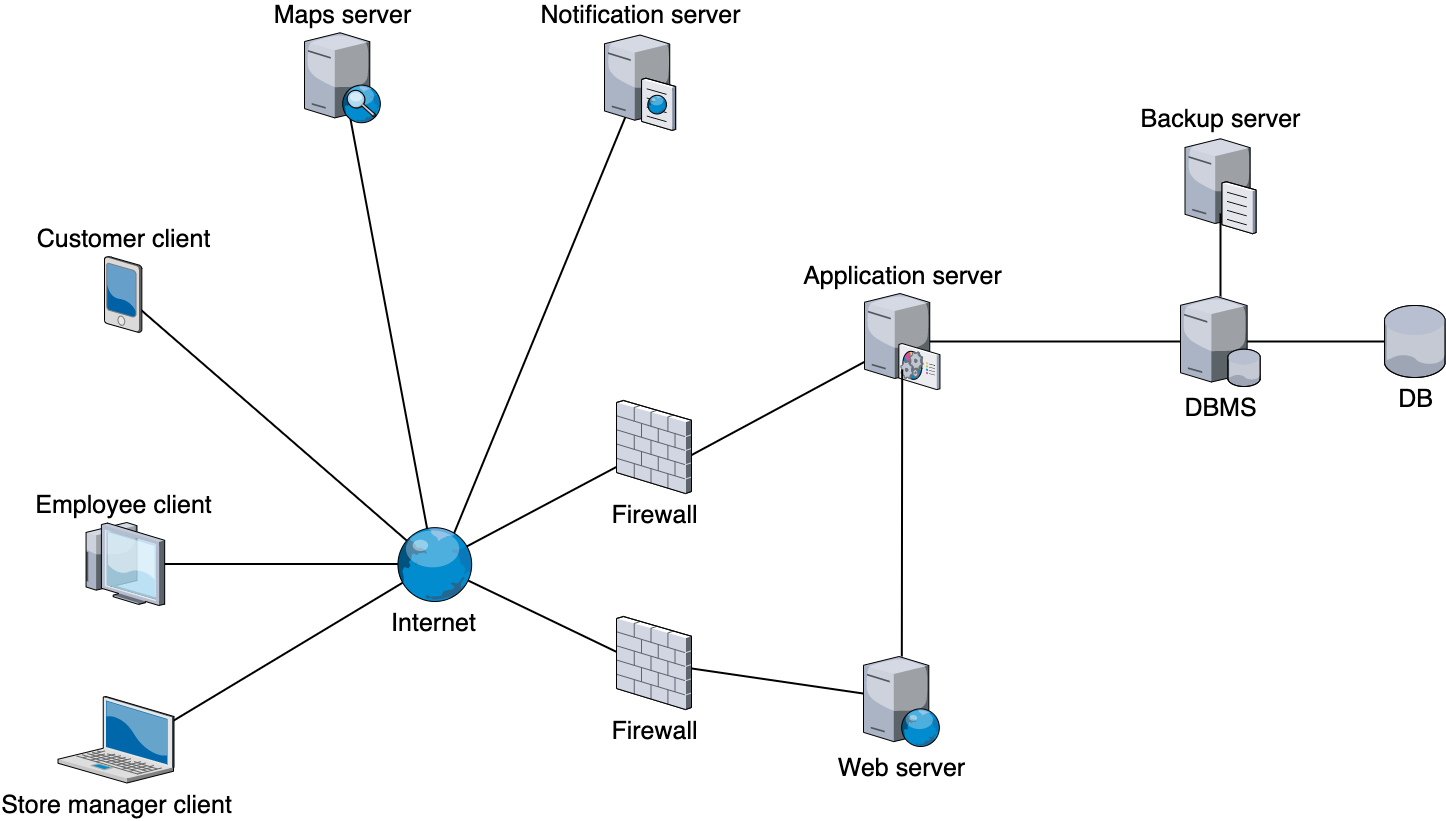
\includegraphics[width=16cm]{high_level_view.png}
\end{figure}

	\section{Component view}

		To make it easier to read component diagrams, it was decided to present 4 diagrams. The first represents a high-level view that reports client-side and server-side components. The other 3 diagrams each represent one of the 3 main subsystems presented in the first diagram.
\subsection{High level component diagram}
    The following diagram shows the main components of the system and the interfaces through which they interact. There are 2 sides:
    \begin{itemize}
        \item The \textbf{client-side} is composed of 2 components: Mobile Application for the customers and Web Application for employees and the store manager
        \item The \textbf{server-side} is the significant part to analyze more thoroughly, here are 3 main subsystems: \begin{itemize}
            \item The \textit{Customer Mobile Services} provides the interfaces to line up, book a visit and manage historical information and account information
            \item The \textit{Employee Web Services} supports the operations that the employee can perform on the web application. This component provides the interfaces to line up (for an external client), to confirm an entrance or an exit from the store
            \item The \textit{Store Manager Web Services} supports the operations that the store manager can perform on the web application. This component provides the interfaces to manage store and employees information and to visualizes data about entrances
        \end{itemize}
    \end{itemize}

    %\begin{figure}[H]
        %\centering
        %\includegraphics[width=16cm]{}
        %\caption{High level component diagram}
    %\end{figure}

\subsection{Customer mobile services diagram}

    The following diagram shows how the subsystem \textbf{Customer Mobile Services} is composed and how its modules communicate with external modules. This subsystem contains 3 modules: a \textit{Visit Reservation Module}, a \textit{Line up Reservation Module} and an \textit{Account Manager}. This modules provides to Mobile Application the following interfaces: \textit{VisitHistory}, \textit{LineUpHistory}, \textit{ManageVisit}, \textit{ManageLineUp}, \textit{ProfileManagement}, \textit{AccessManager}. The components of the Customer Mobile Services subsystem need to communicate with the DBMS, Maps API, OS Notification Gateway, Queue Manager and Visit Scheduler.

    %\begin{figure}[H]
        %\centering
        %\includegraphics[width=16cm]{}
        %\caption{Customer Mobile Services component diagram}
    %\end{figure}

\subsection{Employee web services diagram}

    The following diagram shows how the subsystem \textbf{Employee Web Services} is composed and how its modules communicate with external modules. This subsystem contains 3 modules: a \textit{Line up Reservation Module}, a \textit{Entrances and Exits Module} and an \textit{Account Manager}. This modules provides to Web Application the following interfaces: \textit{LineUp}, \textit{ManageEntrances}, \textit{ManageExits}, \textit{AccessManager}. The components of the Employee Web Services subsystem need to communicate with the DBMS and the Queue Manager.

    %\begin{figure}[H]
        %\centering
        %\includegraphics[width=16cm]{}
        %\caption{Employee Web Services component diagram}
    %\end{figure}

\subsection{Store Manager web services diagram}

    The following diagram shows how the subsystem \textbf{Store Manager Web Services} is composed and how its modules communicate with external modules. This subsystem contains 3 modules: a \textit{Statistics and Data Gateway}, a \textit{Store Info and Employees Manager} and an \textit{Account Manager}. This modules provides to Web Application the following interfaces: \textit{Retrieve Statistics}, \textit{StoreManagement}, \textit{ProfileManagement}, \textit{AccessManager}. The components of the Store Manager Web Services subsystem need to communicate with the DBMS.

    %\begin{figure}[H]
        %\centering
        %\includegraphics[width=16cm]{}
        %\caption{Store Manager Web Services component diagram}
    %\end{figure}

	\section{Deployment view}

		The system architecture is divided into 5 tiers and it's implemented using the Java Enterprise Edition framework.
\begin{itemize}
    \item The first tier is the client tier: it contains the mobile application running on customers' devices and the web browser used by the store employees and the store manager to access the web application of CLup. The former communicates with the JEE server via a REST interface. The latter accesses the webserver and retrieves web pages.
    \item The second tier is the web tier: it is composed of the webserver implemented with the Apache HTTP platform. It mainly serves the static content and it is connected with the Tomcat script server to load the dynamic data.
    \item The third tier contains the script engine server. Tomcat has been chosen as the platform to generate dynamic content, via Servlet or JSP, requested by the Apache HTTP server.
    \item The fourth tier is the application logic tier: it is composed of the WildFly application server platform which handles the Enterprise Java Beans to which the Tomcat server connects.
    \item On the data tier (tier 5) there is the Database server. The connection with tier 4 is implemented with a JDBC connector.
\end{itemize}

\begin{figure}[H]
    \centering
    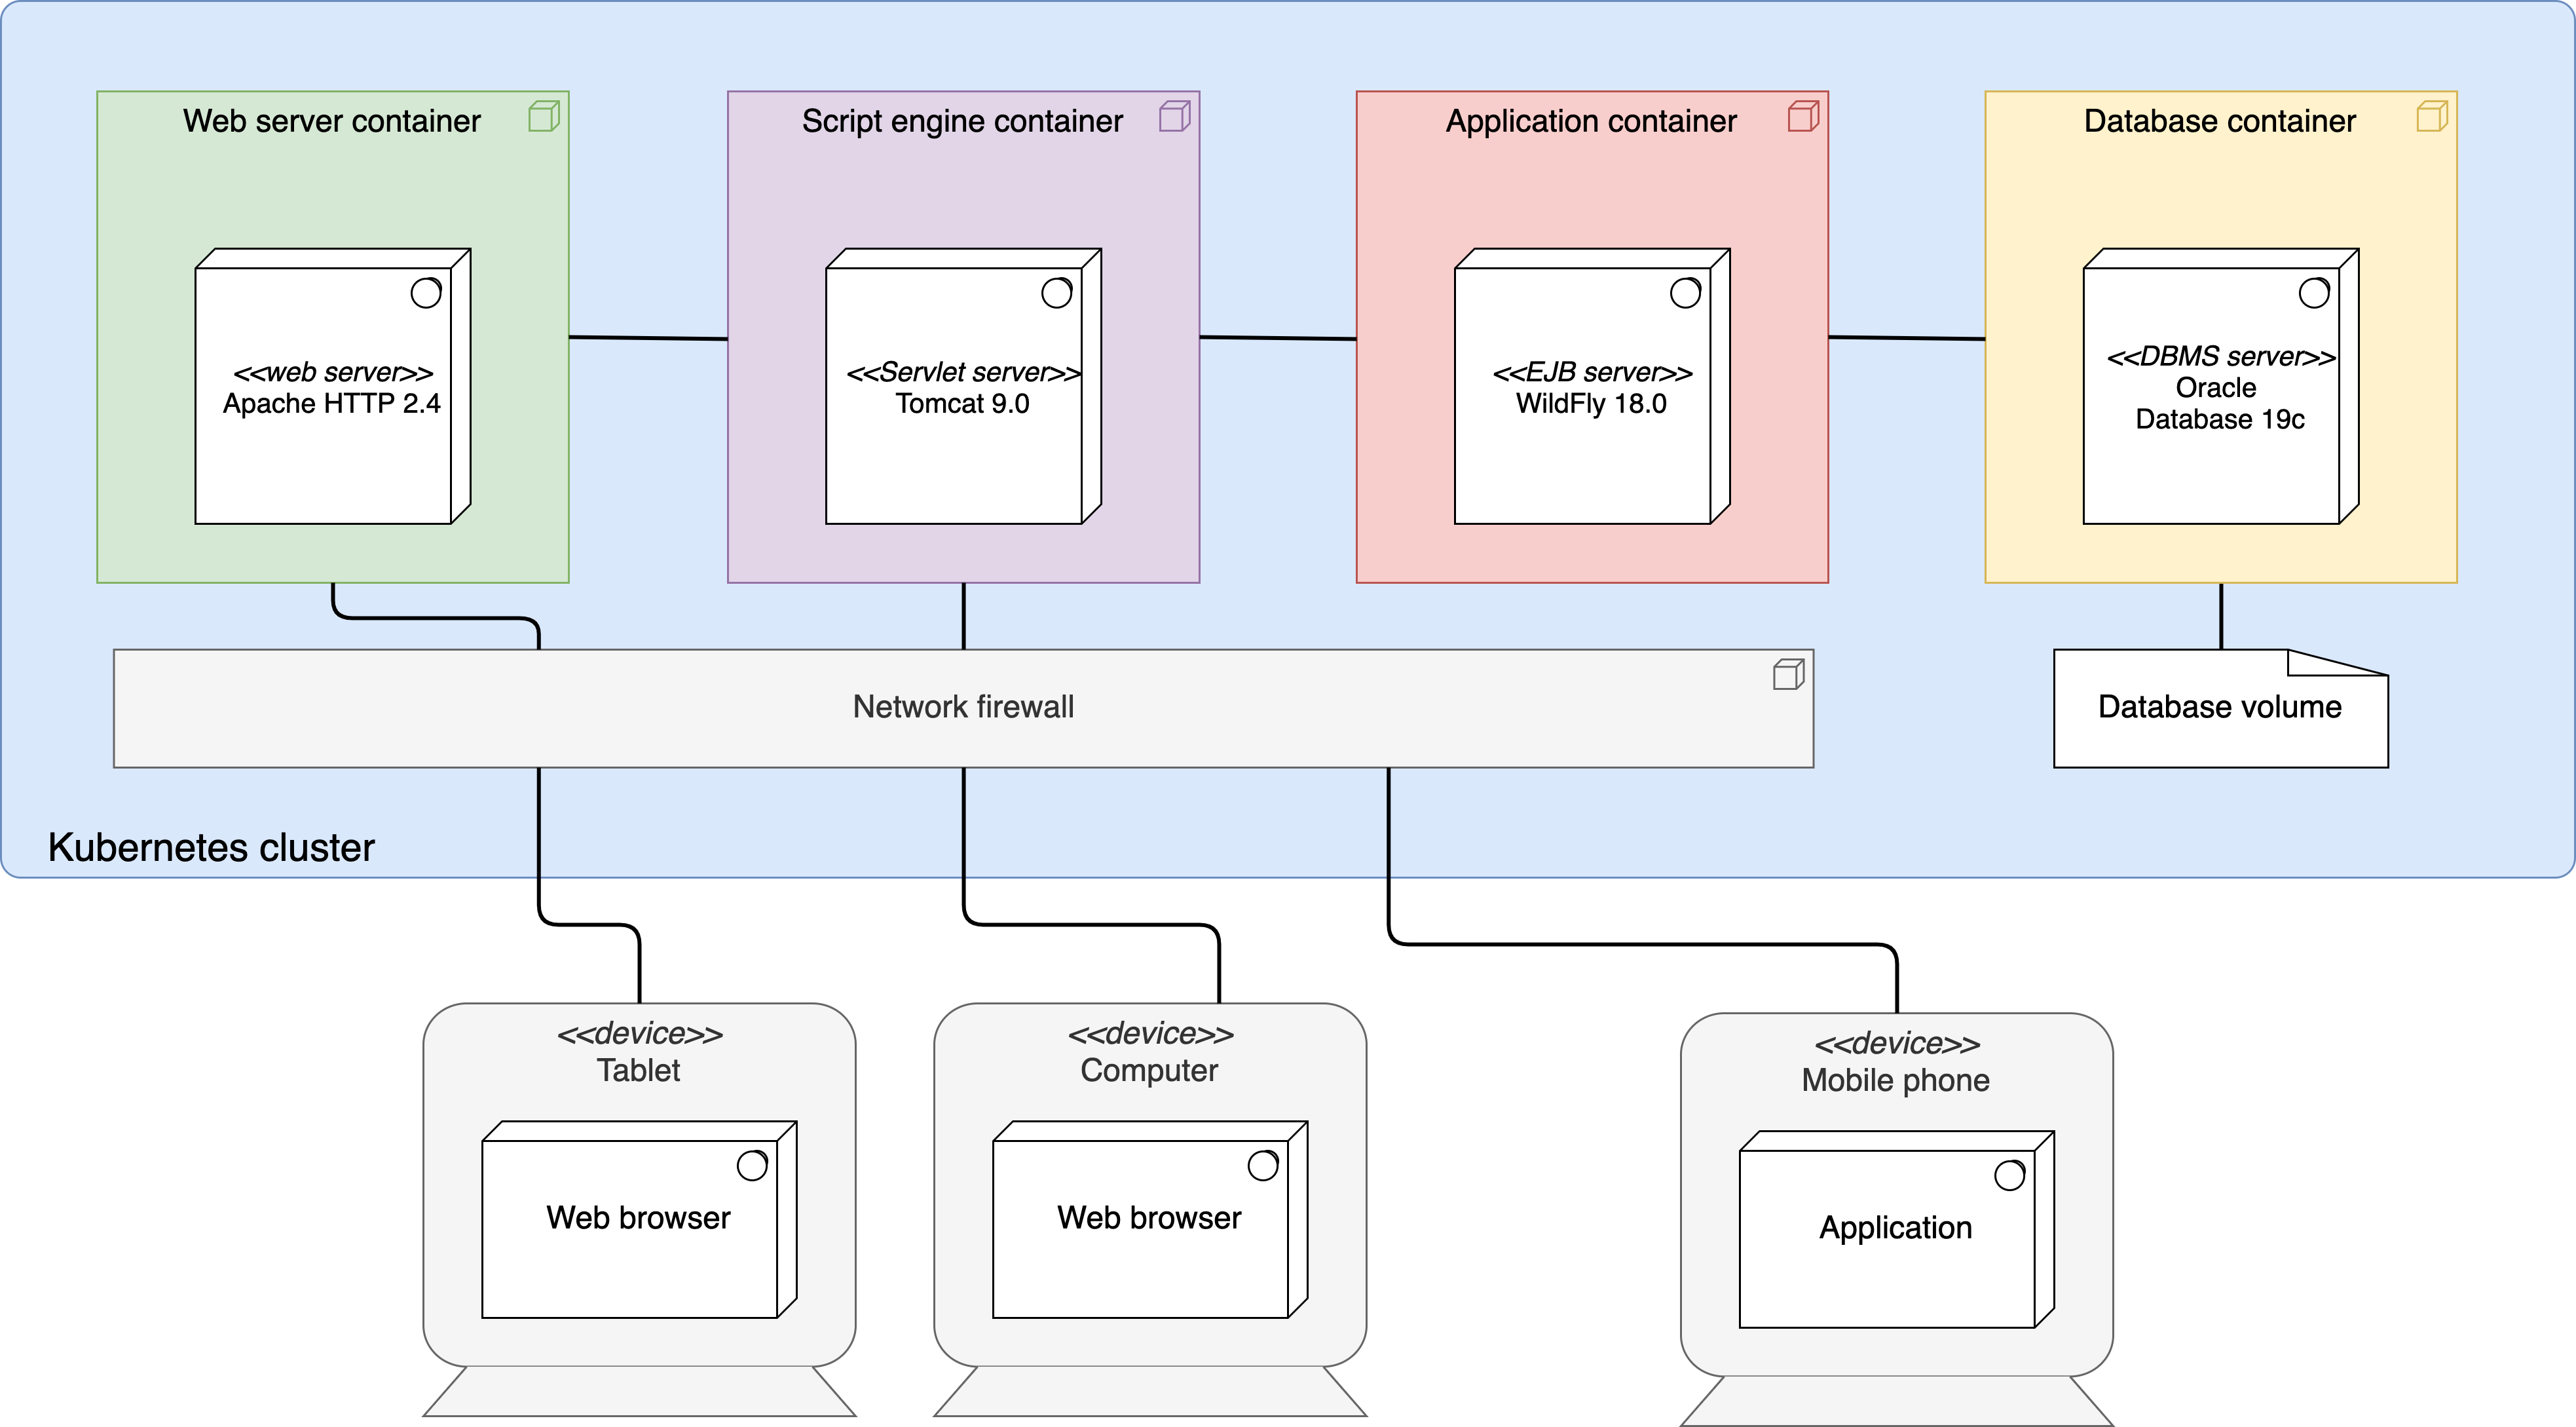
\includegraphics[width=16cm]{deployment_view.png}
    \caption{Deployment diagram}
\end{figure} 

\textbf{Recommended deployment:}

All the tiers, except the first one, must be deployed as containers in a Kubernetes cluster. Each of the four tiers may be containerized and then deployed in a cluster. This process would produce many advantages such as:
\begin{itemize}
    \item Easy replication management: it as easy as to change a number in a configuration file to scale up or down one of the tiers (except for the database, which is a little bit more involved).
    \item Portability: the application is extremely portable between different physical or cloud deployments, for example, allowing to switch between geographically different datacenters in a couple of minutes.
    \item Easy update management: update release is only a matter of shutting down some containers and bringing up new ones from updated images. Moreover, different versions of the system can coexist at the same time on the same cluster.
\end{itemize}
The Kubernetes cluster may be created and managed by the CLup deployment team. A better option may be to directly deploy the containers to Amazon EKS, Google Kubernetes Engine, or similar cloud services. In the latter case, tier 5 may use a service like Amazon EFS or Google Firestore to store the database, allowing to make copies of the database and protect against hard failures with an automatic backup solution offered by those cloud providers.

\bigbreak
\textbf{Recommended implementation:}
\begin{itemize}
    \item \textbf{Client tier:} the customer mobile application may be implemented using a cross-platform development framework like Flutter. Flutter allows writing the application code once and then to easily compile the source code for both Android and iOS systems. This would be a big advantage in terms of reducing development cost and time and of obtaining code maintainability. 
    \item \textbf{Web tier:} the web pages of the web application may be implemented with HTML 5.0, CSS, and JavaScript. 
    \item \textbf{Script engine tier:} the dynamic content may be generated using Java Servlets
    \item \textbf{Application logic tier:} the EJB application server may use stateless Java Beans connected using JPA with the Database server. This would allow having the client state completely stored on the DBMS, thus allowing to easily scale up or down the business instances.
    \item \textbf{Data tier:} the database may be implemented with MySQL Server Enterprise Edition.
\end{itemize}

	\section{Runtime view}

		In the following sequence diagrams, we are going to explain and represent the interactions that happen between the main components of CLup. This is still a high-level description of the actual interactions that will be developed. Thus function names, results, errors, and other details will be modified or added during the development process. 

\begin{figure}[H]
    \centering
    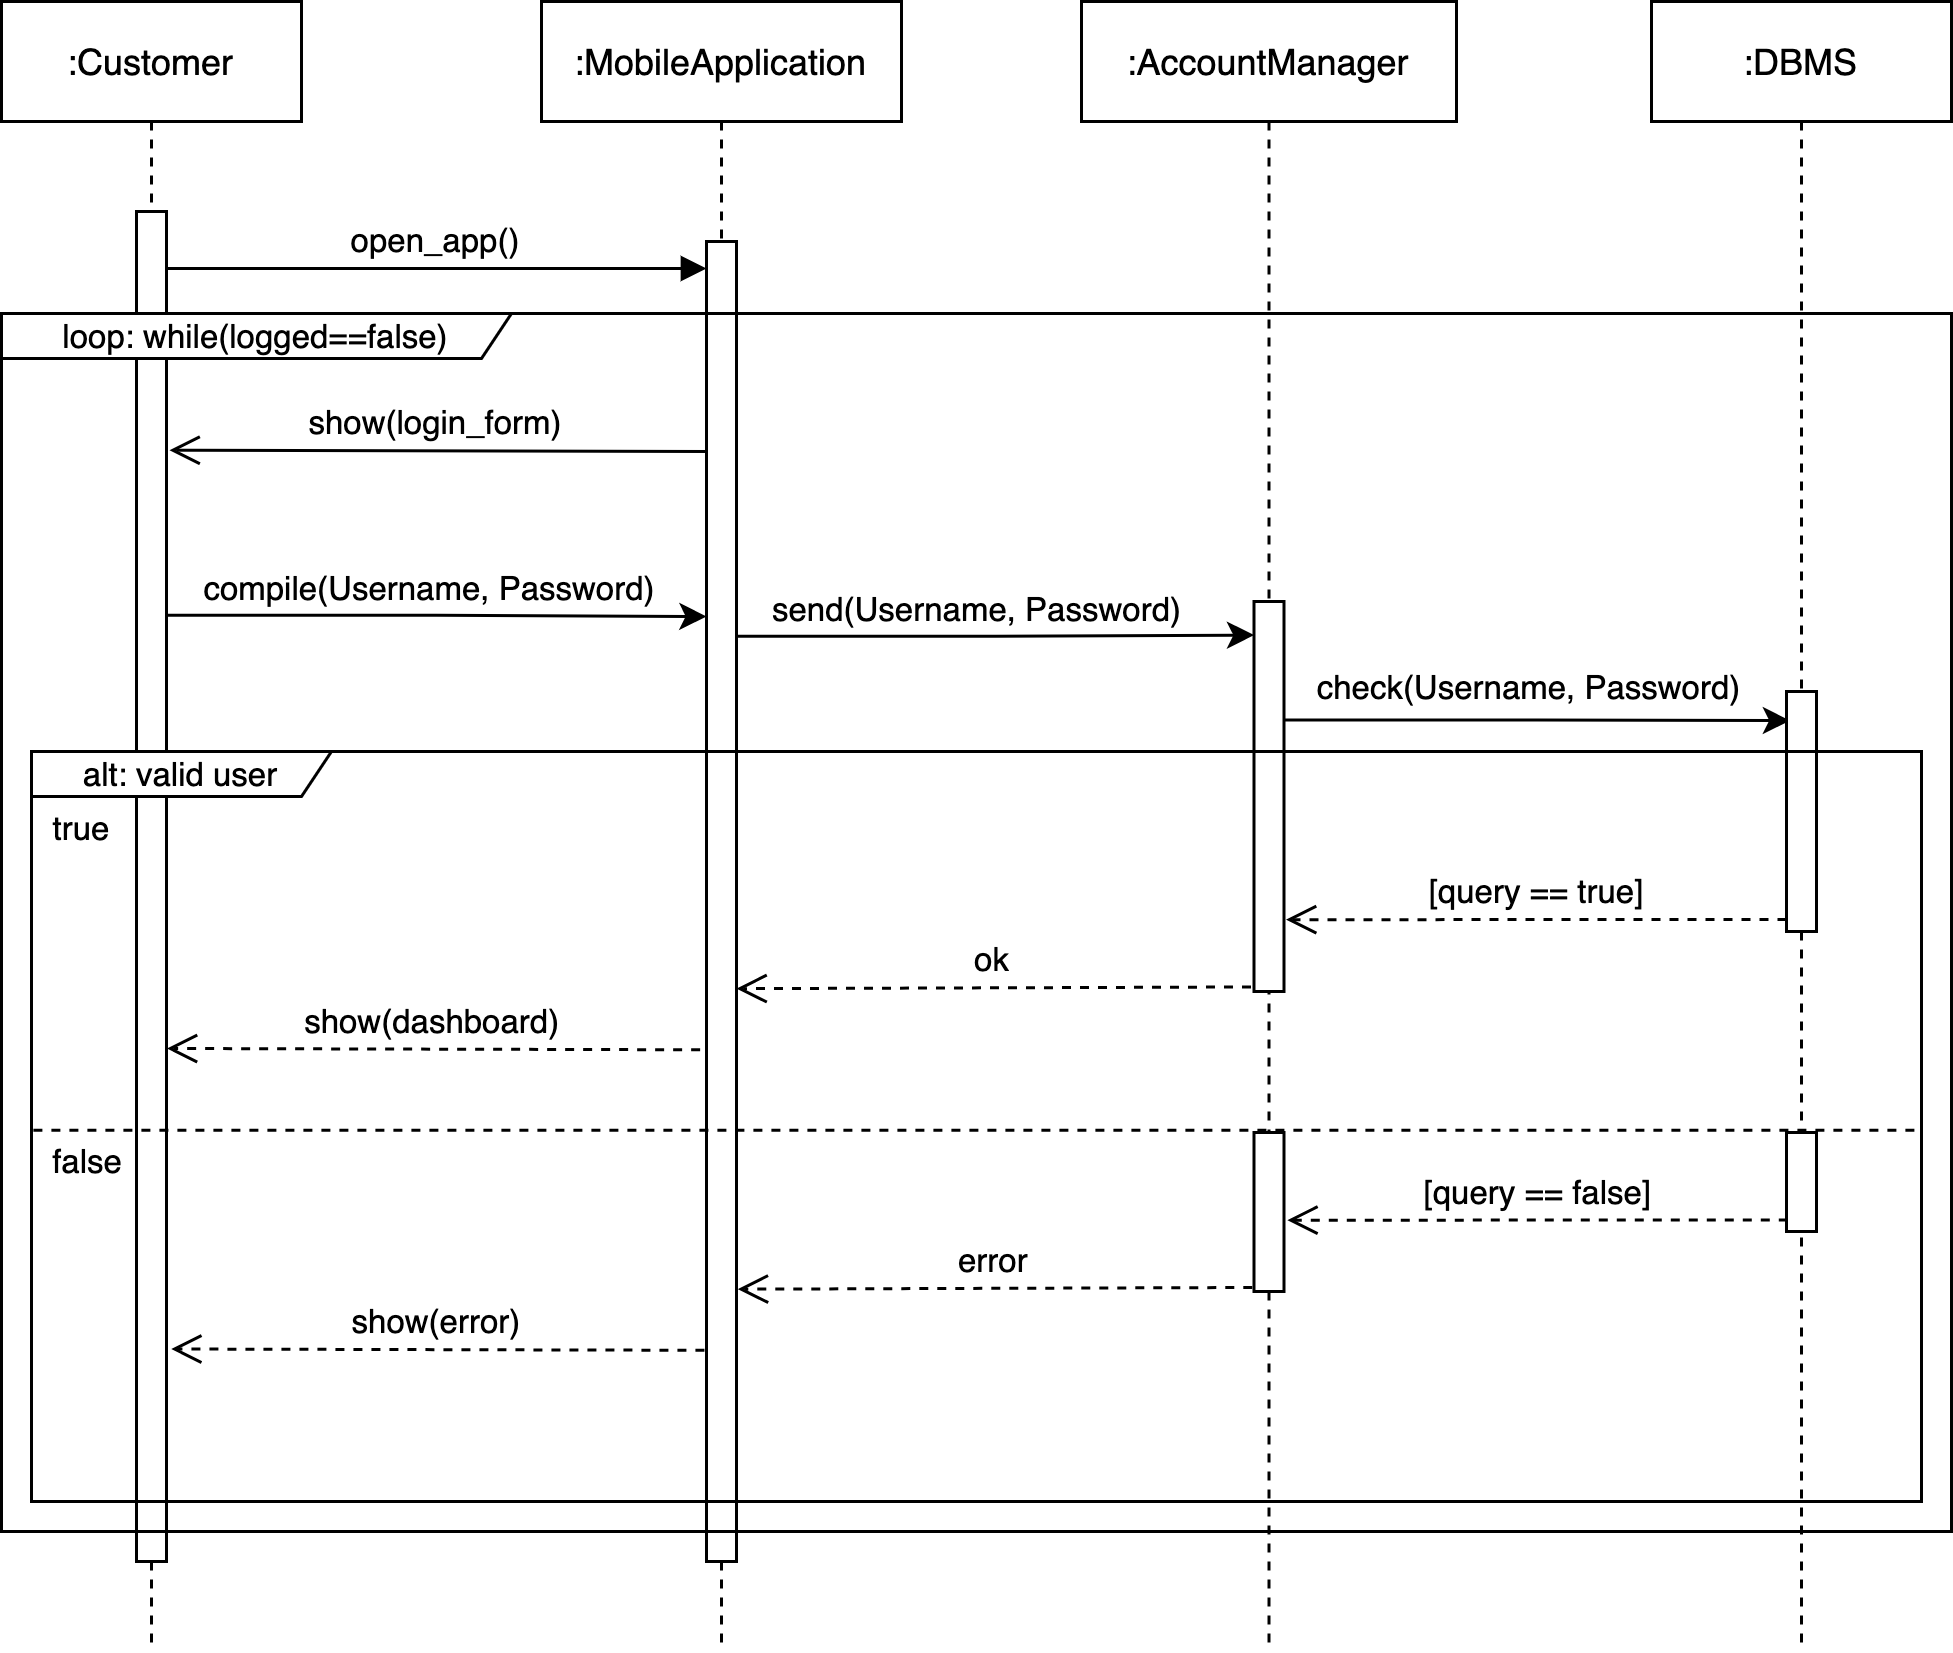
\includegraphics[width=16cm]{runtime_view-Login.png}
    \caption{Customer Login}
\end{figure}

\begin{figure}[H]
    \centering
    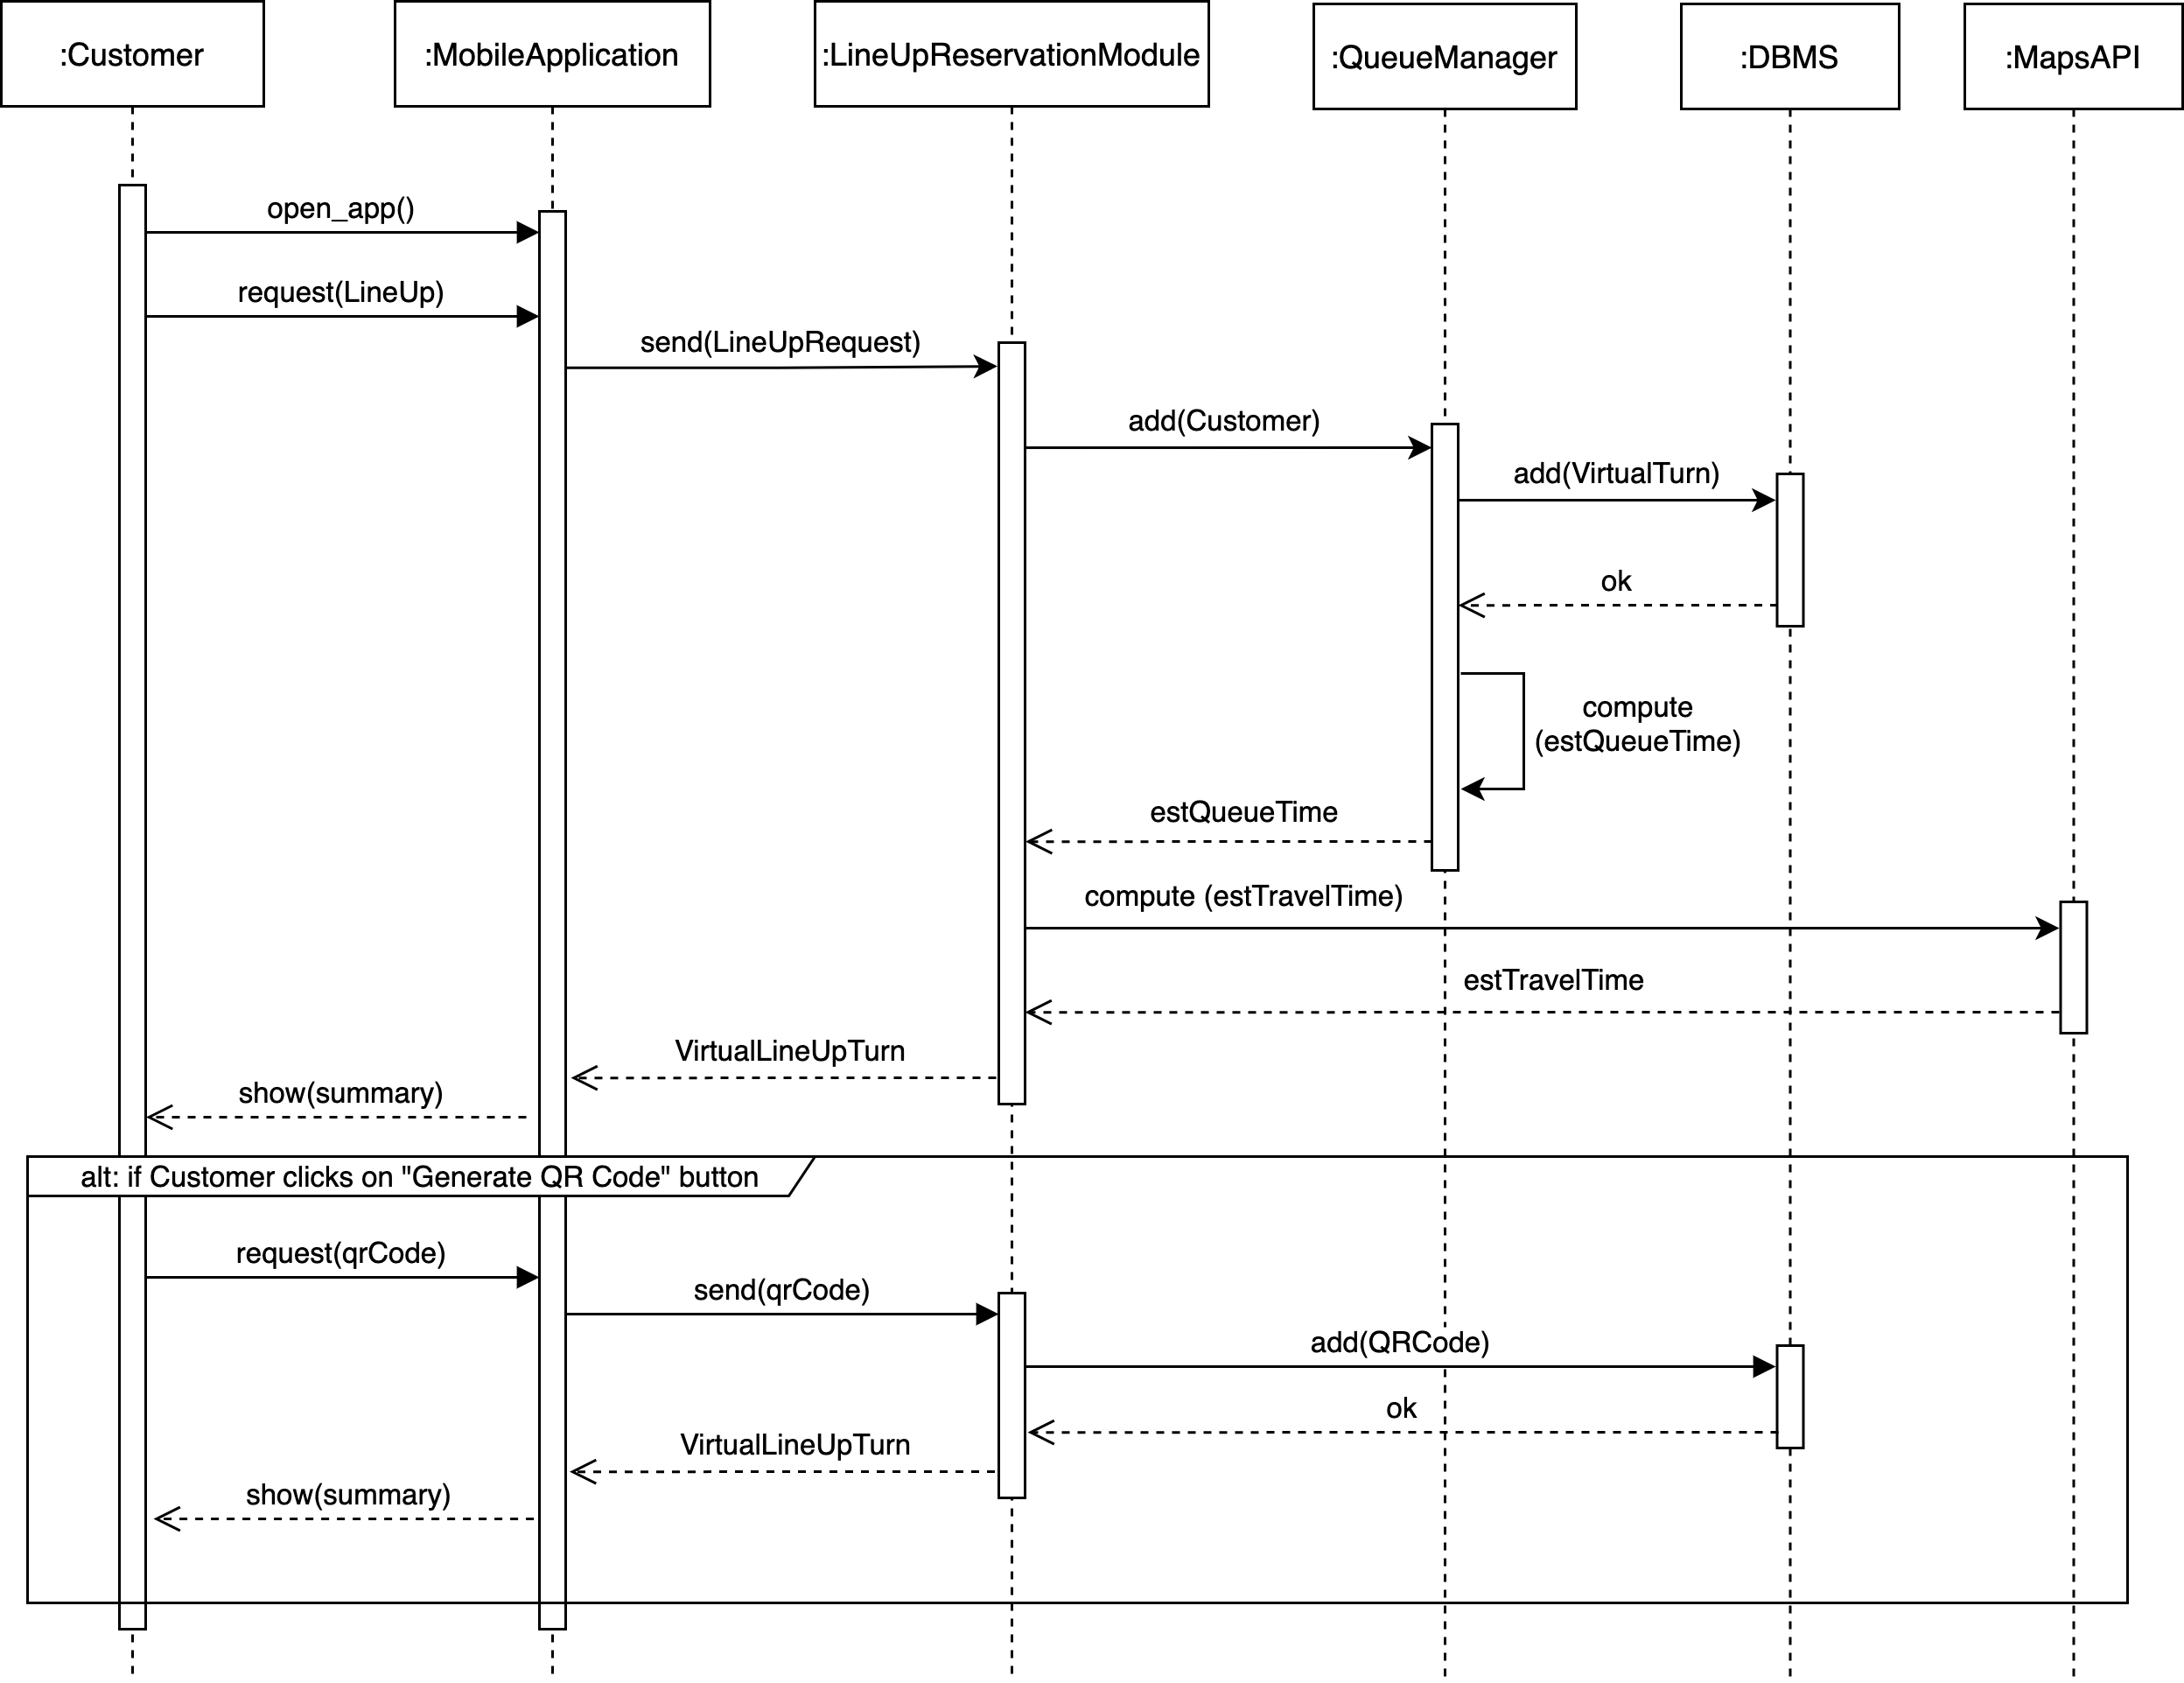
\includegraphics[width=16cm]{runtime_view-LineUpApp.png}
    \caption{Lineup via application}
\end{figure}

\begin{figure}[H]
    \centering
    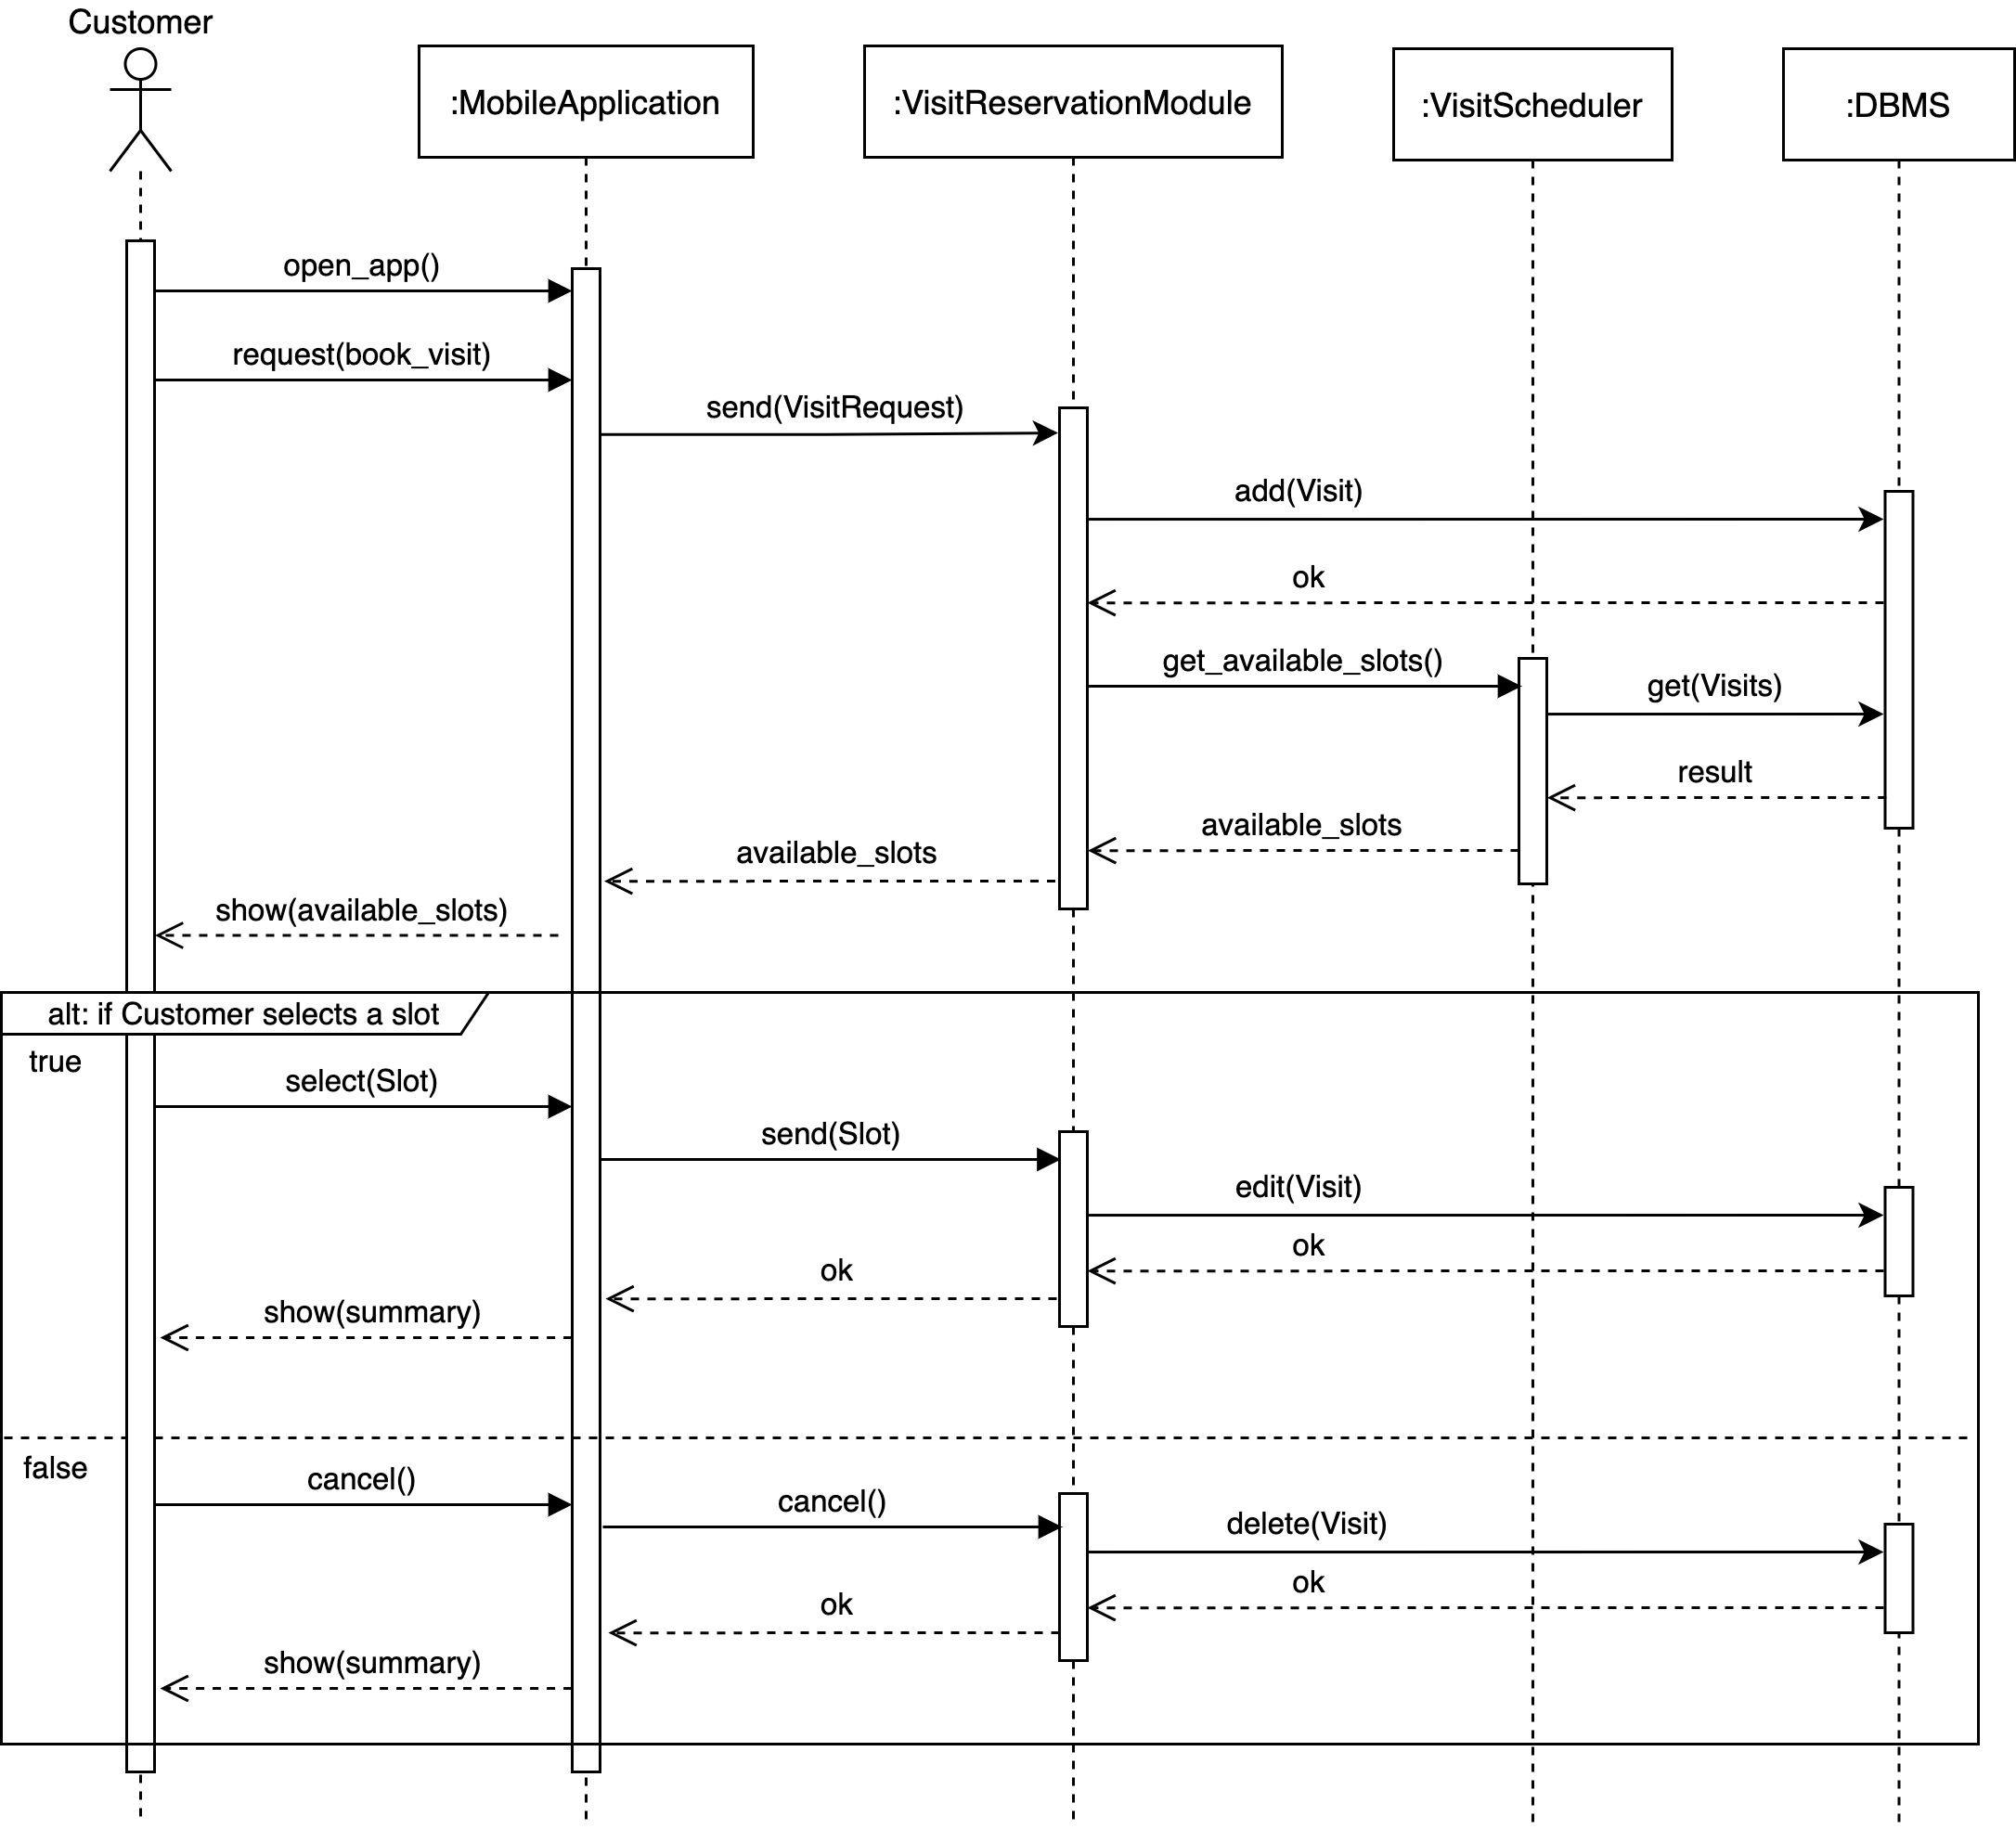
\includegraphics[width=16cm]{runtime_view-BookVisit.png}
    \caption{Book a visit}
\end{figure}

\begin{figure}[H]
    \centering
    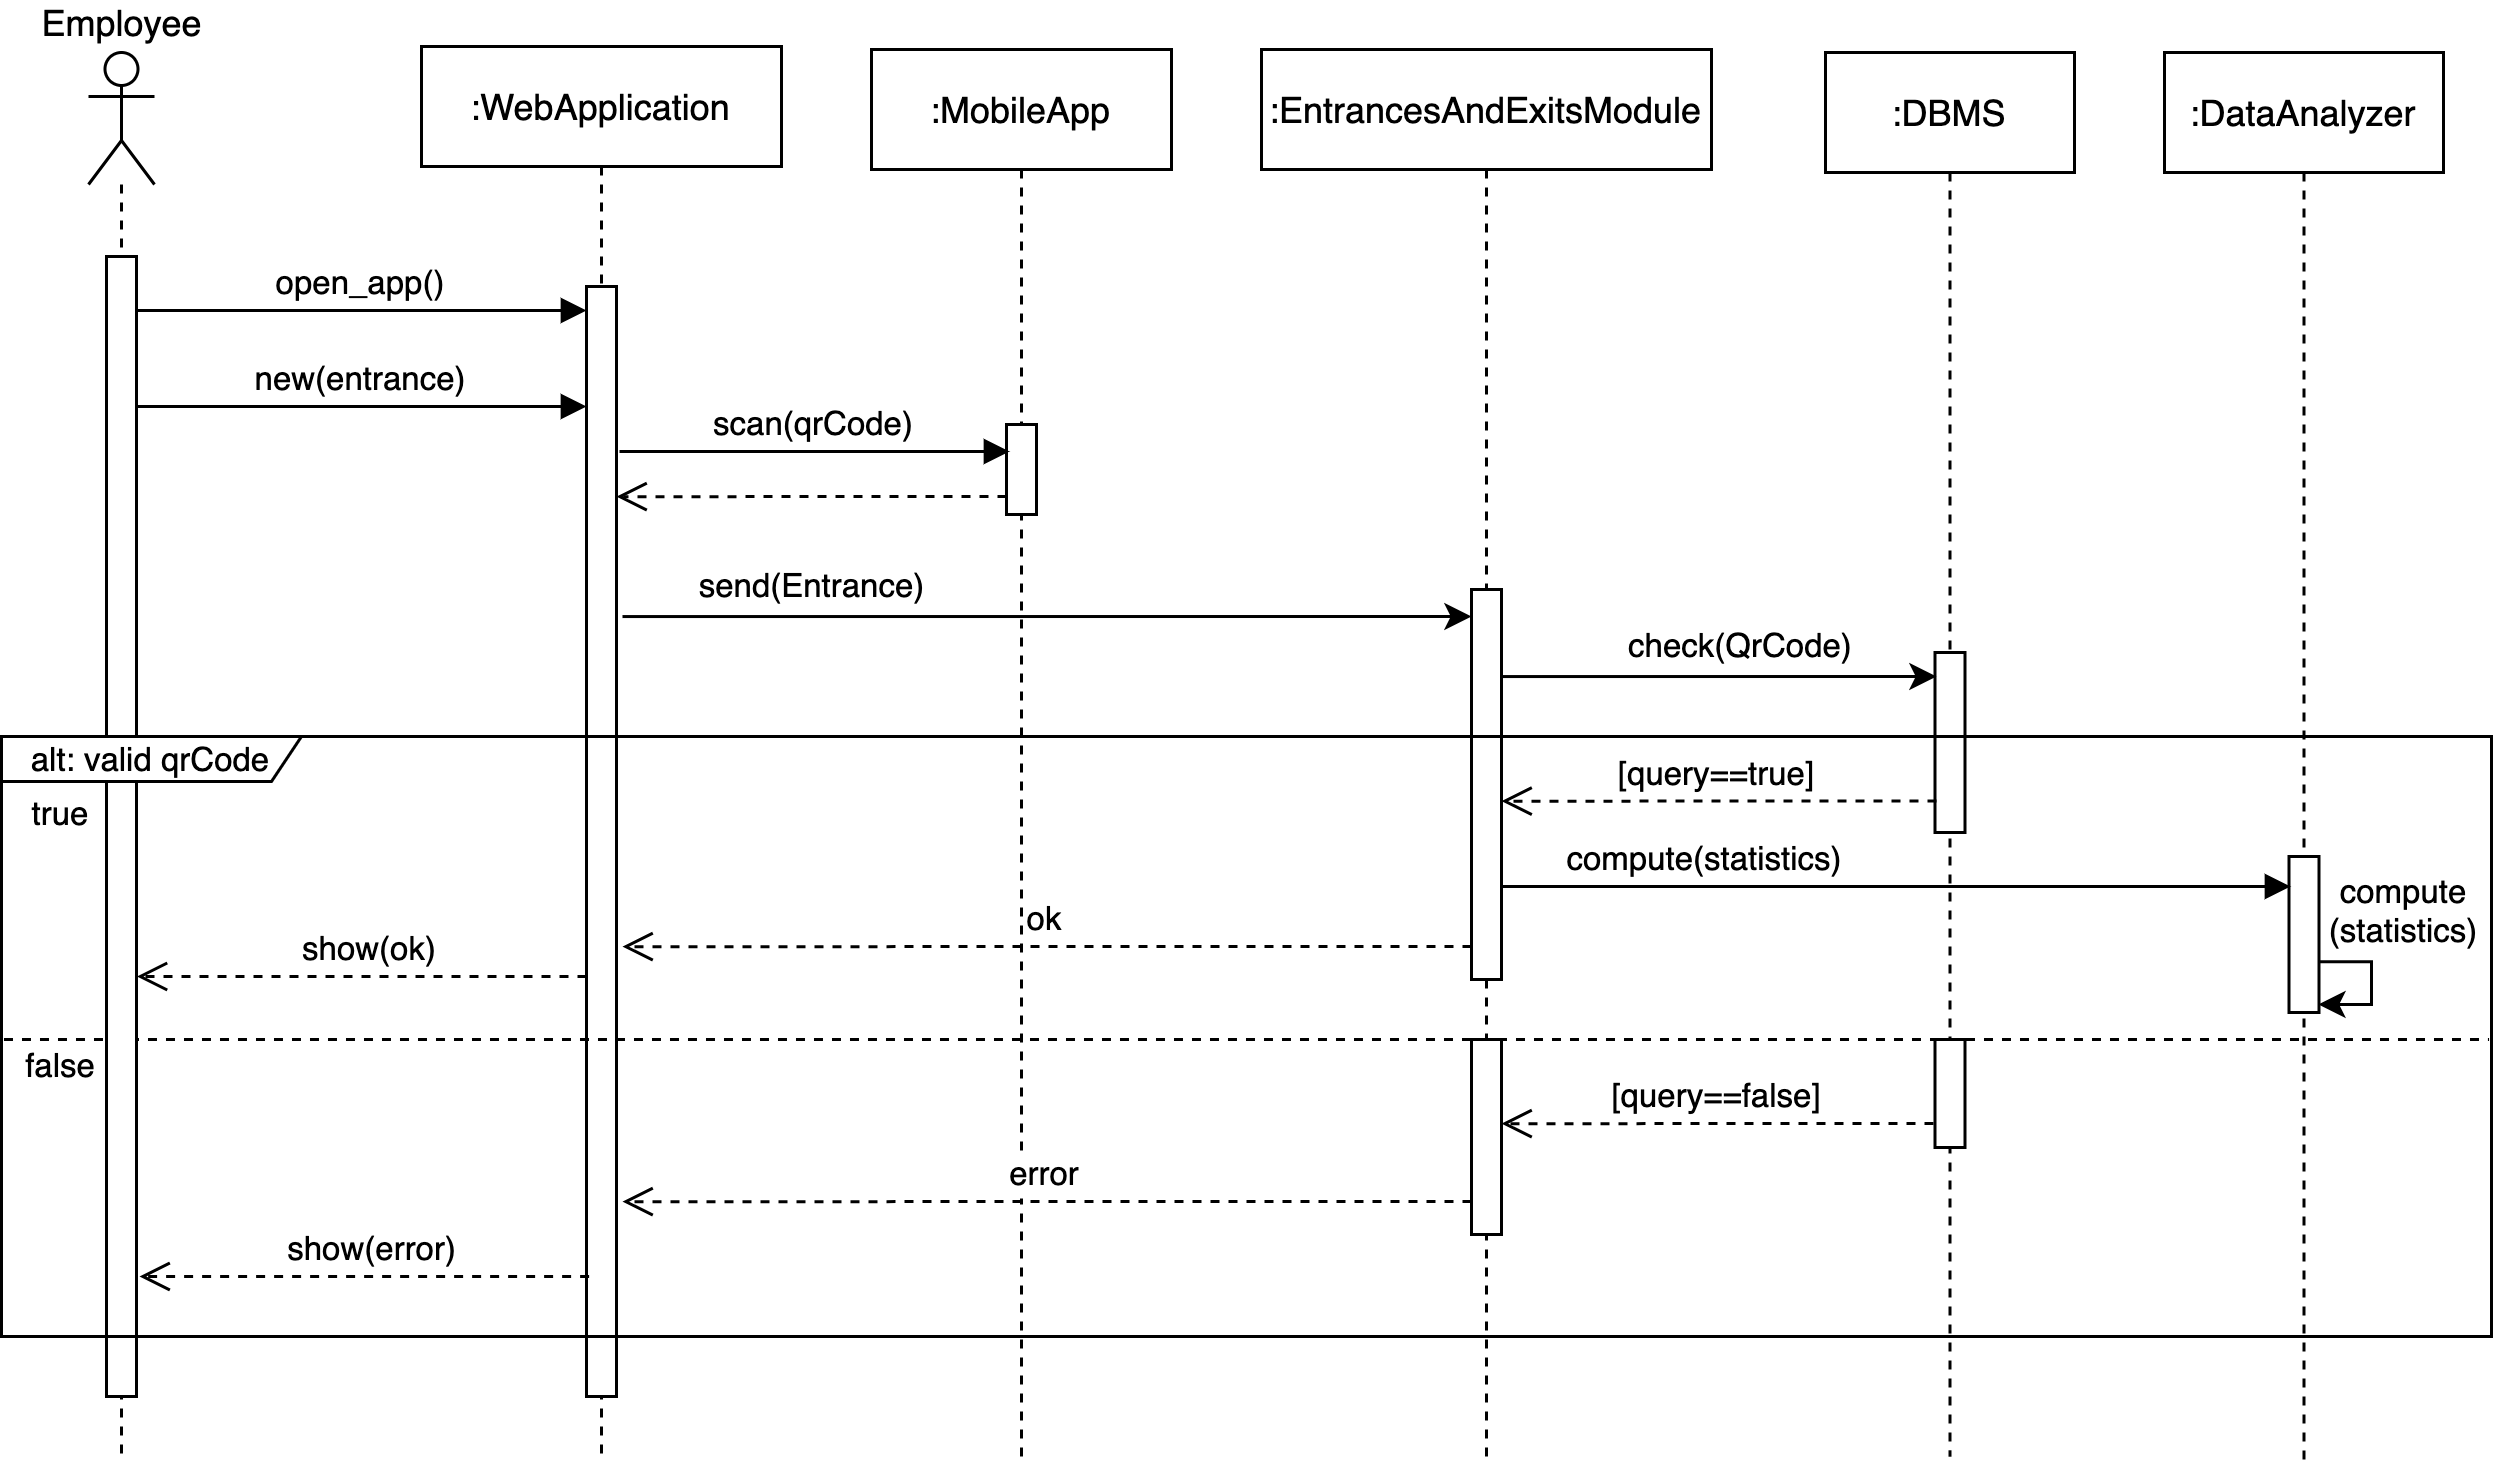
\includegraphics[width=16cm]{runtime_view-qrCodeEntrance.png}
    \caption{Entrance with a QR Code}
\end{figure}

\begin{figure}[H]
    \centering
    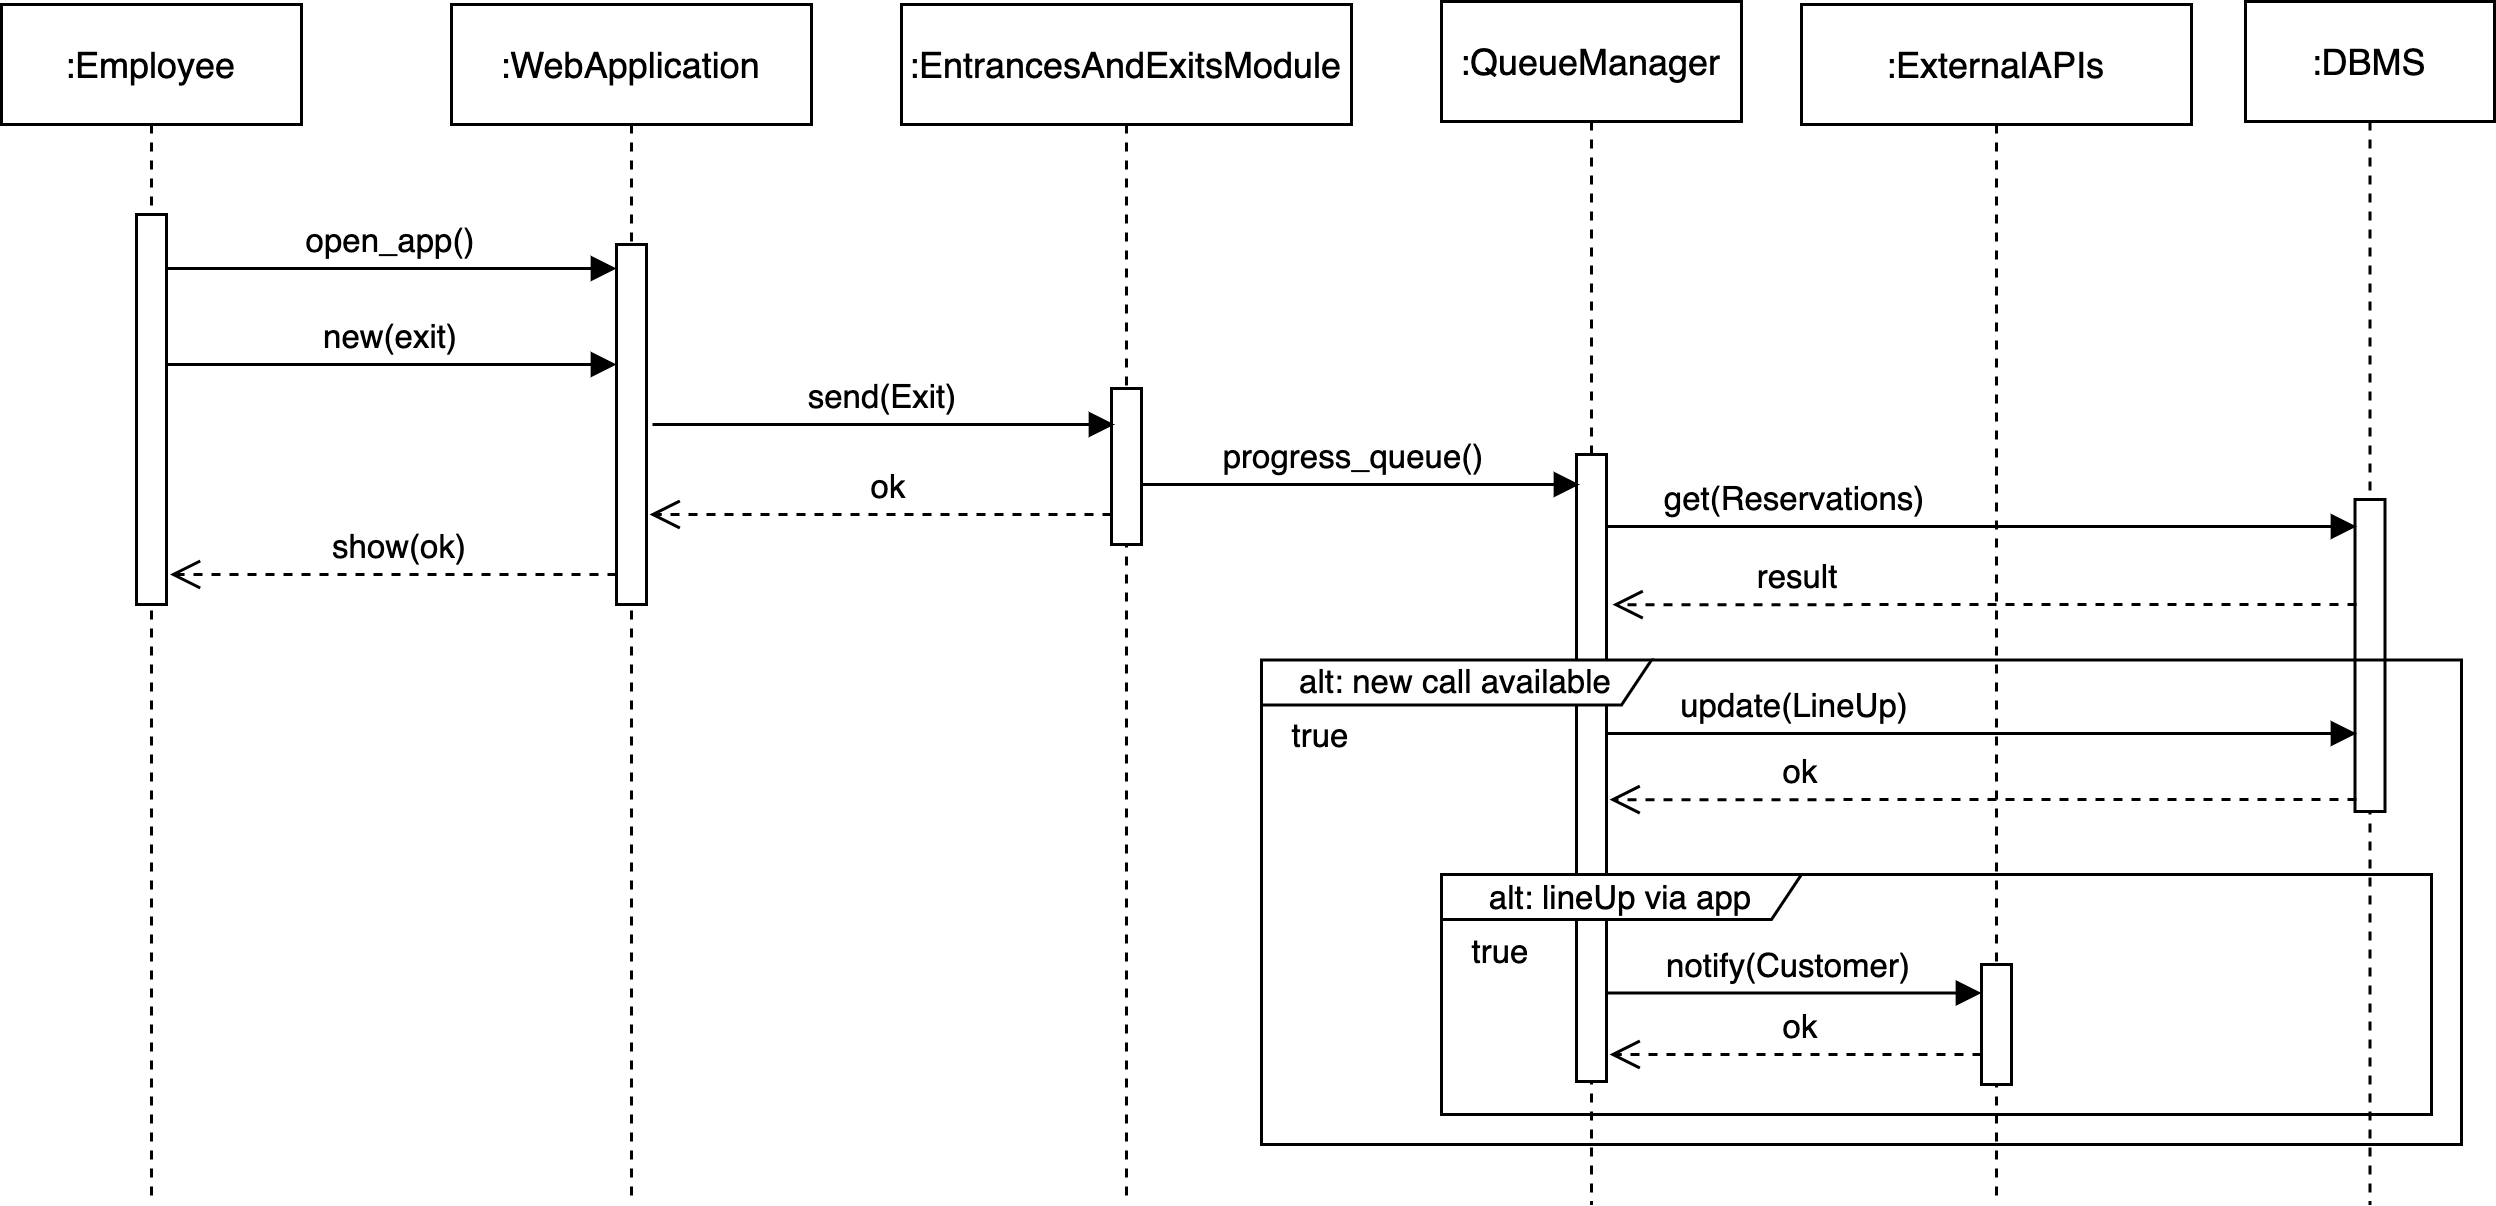
\includegraphics[width=16cm]{runtime_view-ReportExit.png}
    \caption{Exit report}
\end{figure}

\begin{figure}[H]
    \centering
    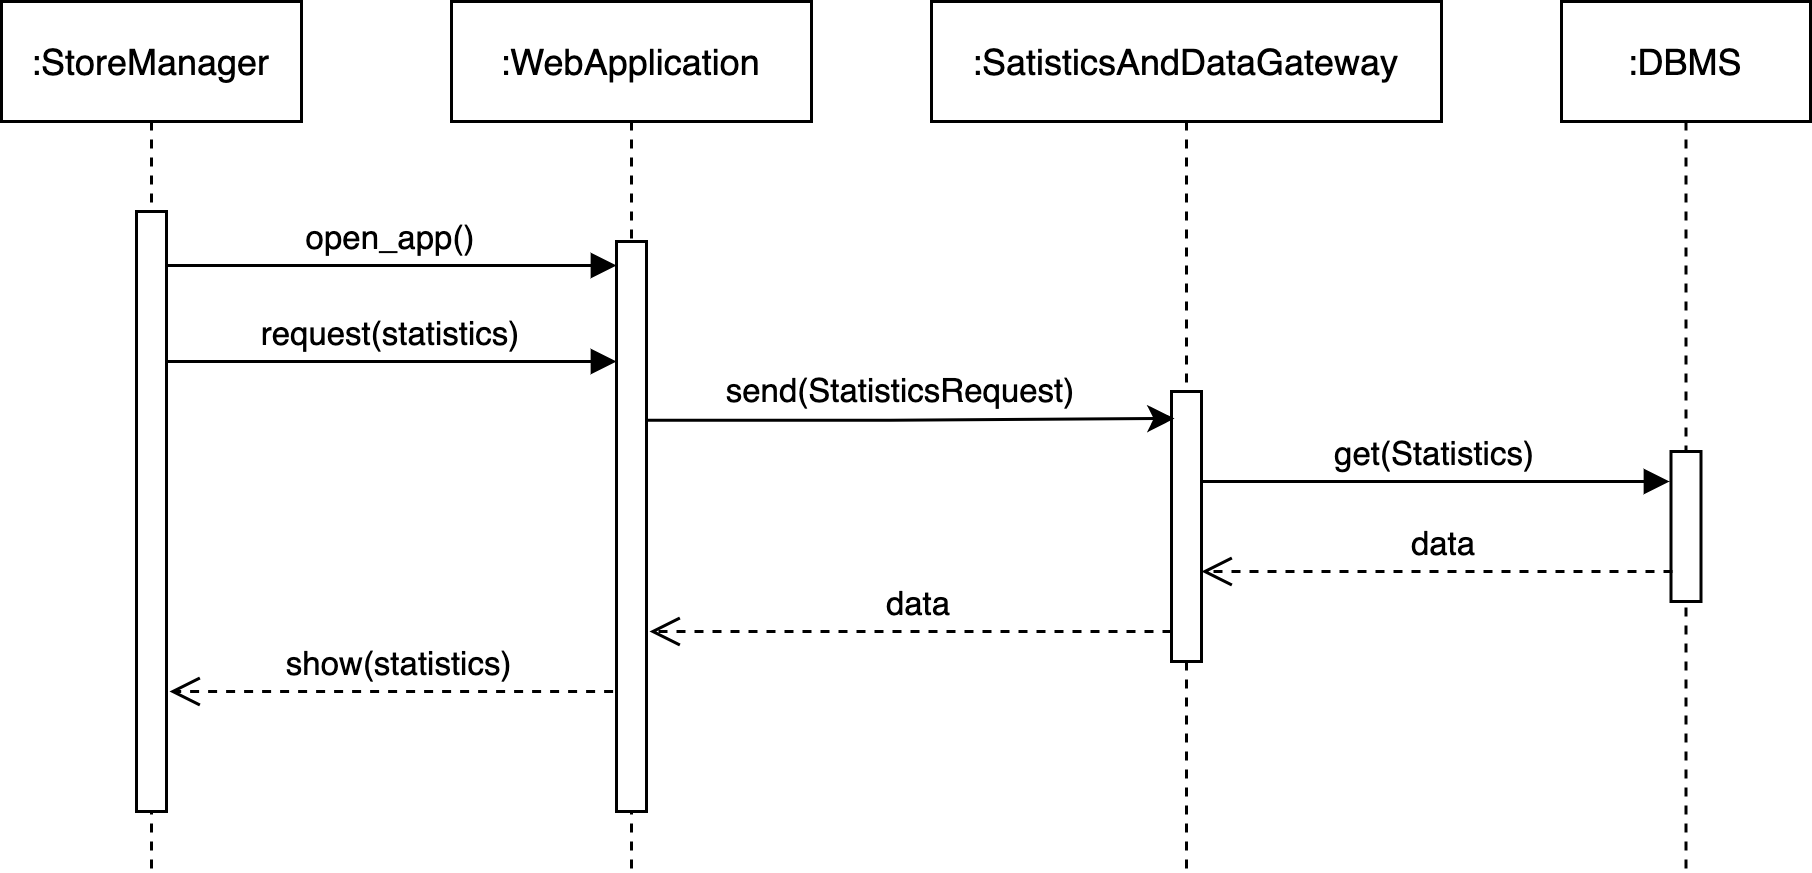
\includegraphics[width=16cm]{runtime_view-Statistics.png}
    \caption{Statistics and charts visualization}
\end{figure}

	\section{Component interfaces}

		In this section the interfaces of the components are analyzed, defining the methods of accessing them. To ensure greater readability, below are three diagrams divided into three diagrams for each susbsystem of the server-side of our system.

\begin{figure}[H]
    \centering
    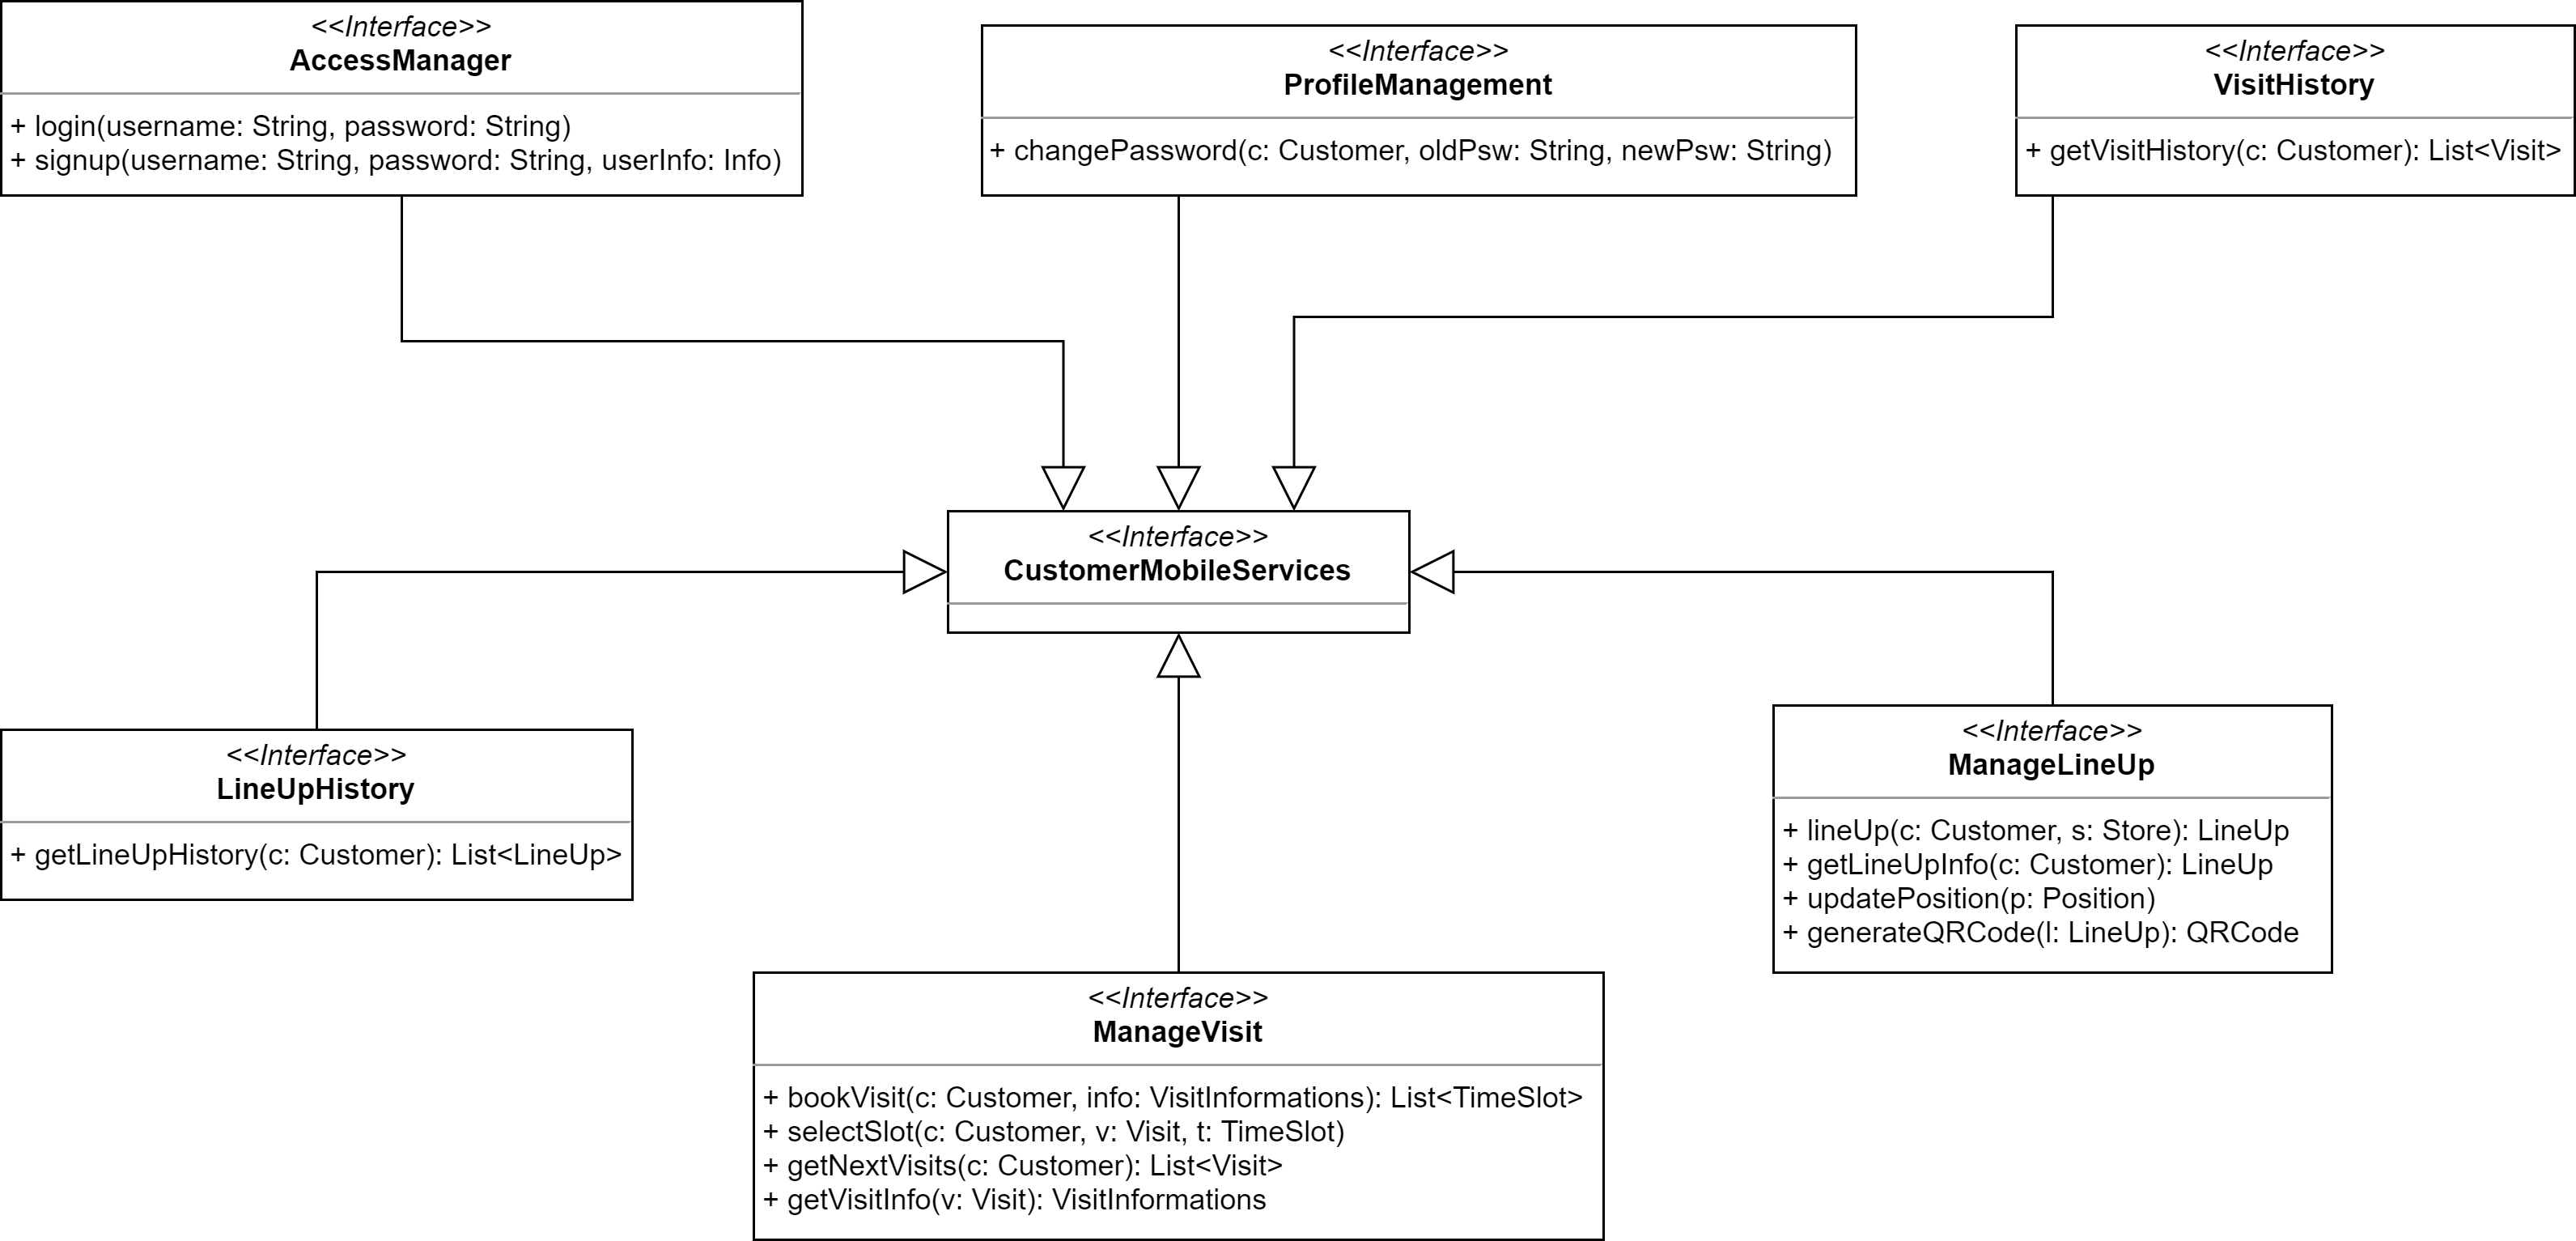
\includegraphics[width=16cm]{cust_mobile_serv_interfaces.png}
    \caption{Customer Mobile Services interfaces}
\end{figure}

\begin{figure}[H]
    \centering
    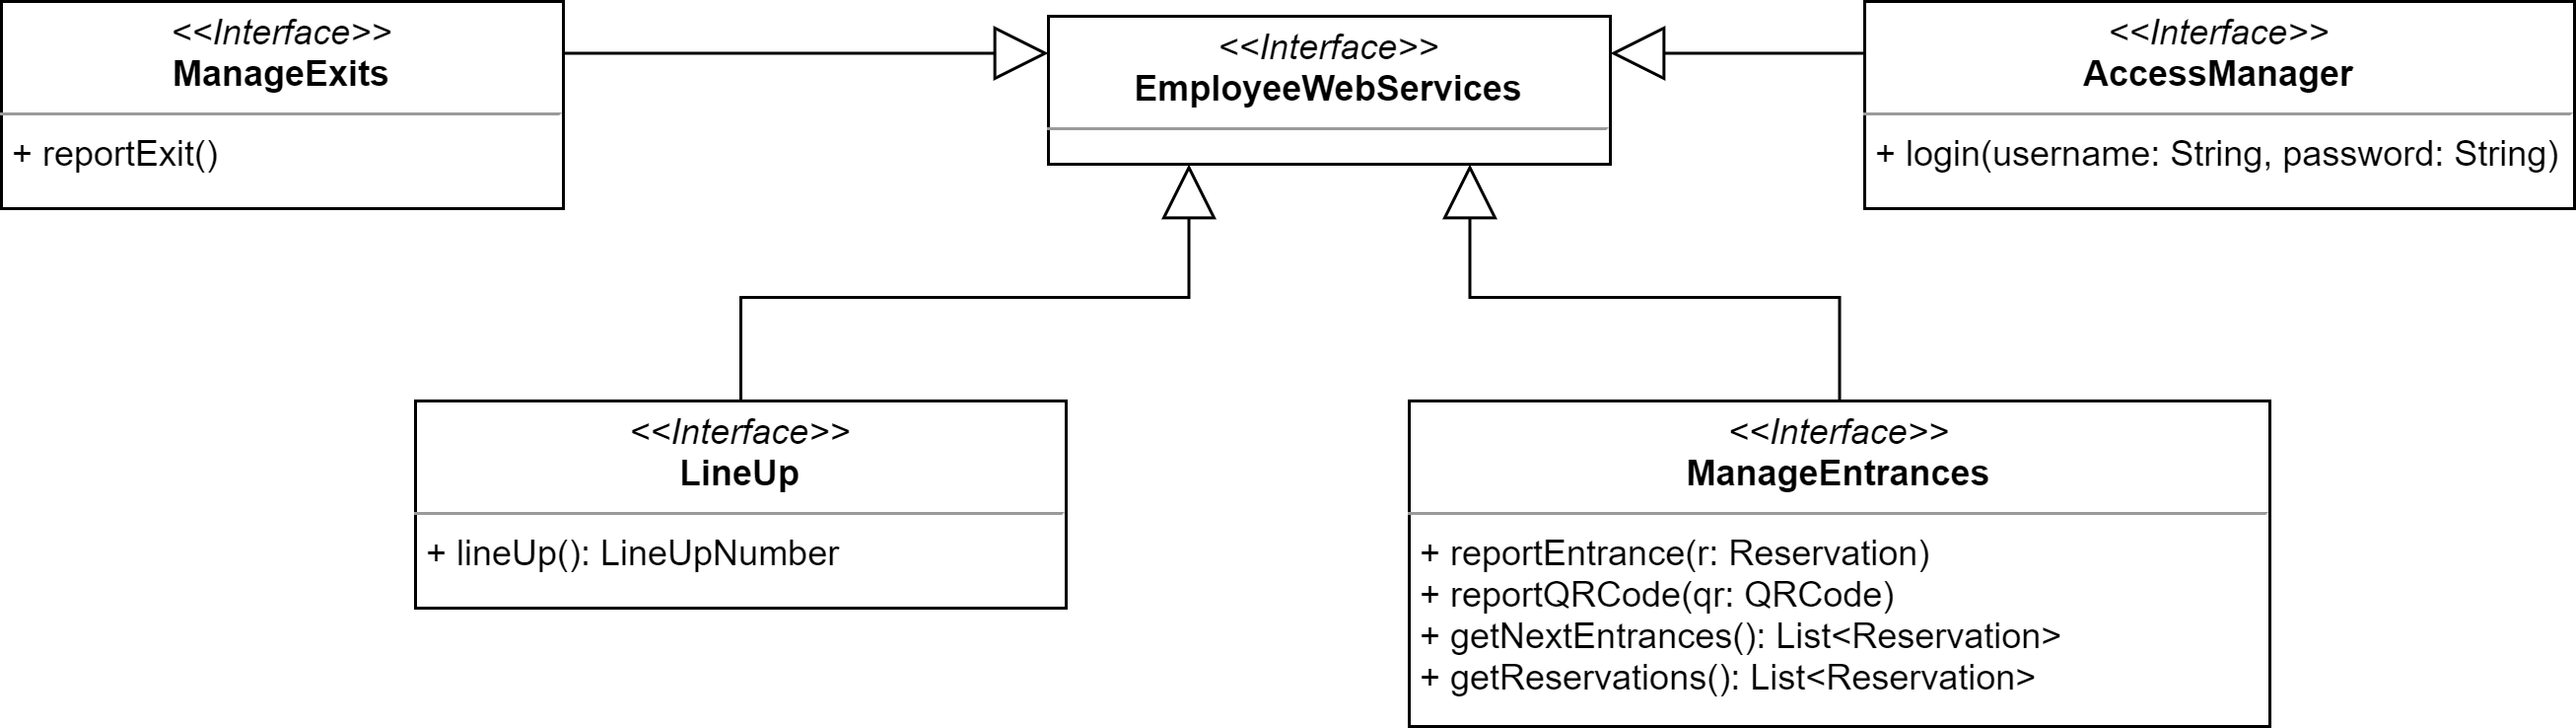
\includegraphics[width=16cm]{empl_web_services_interfaces.png}
    \caption{Employee Web Services interfaces}
\end{figure}

\begin{figure}[H]
    \centering
    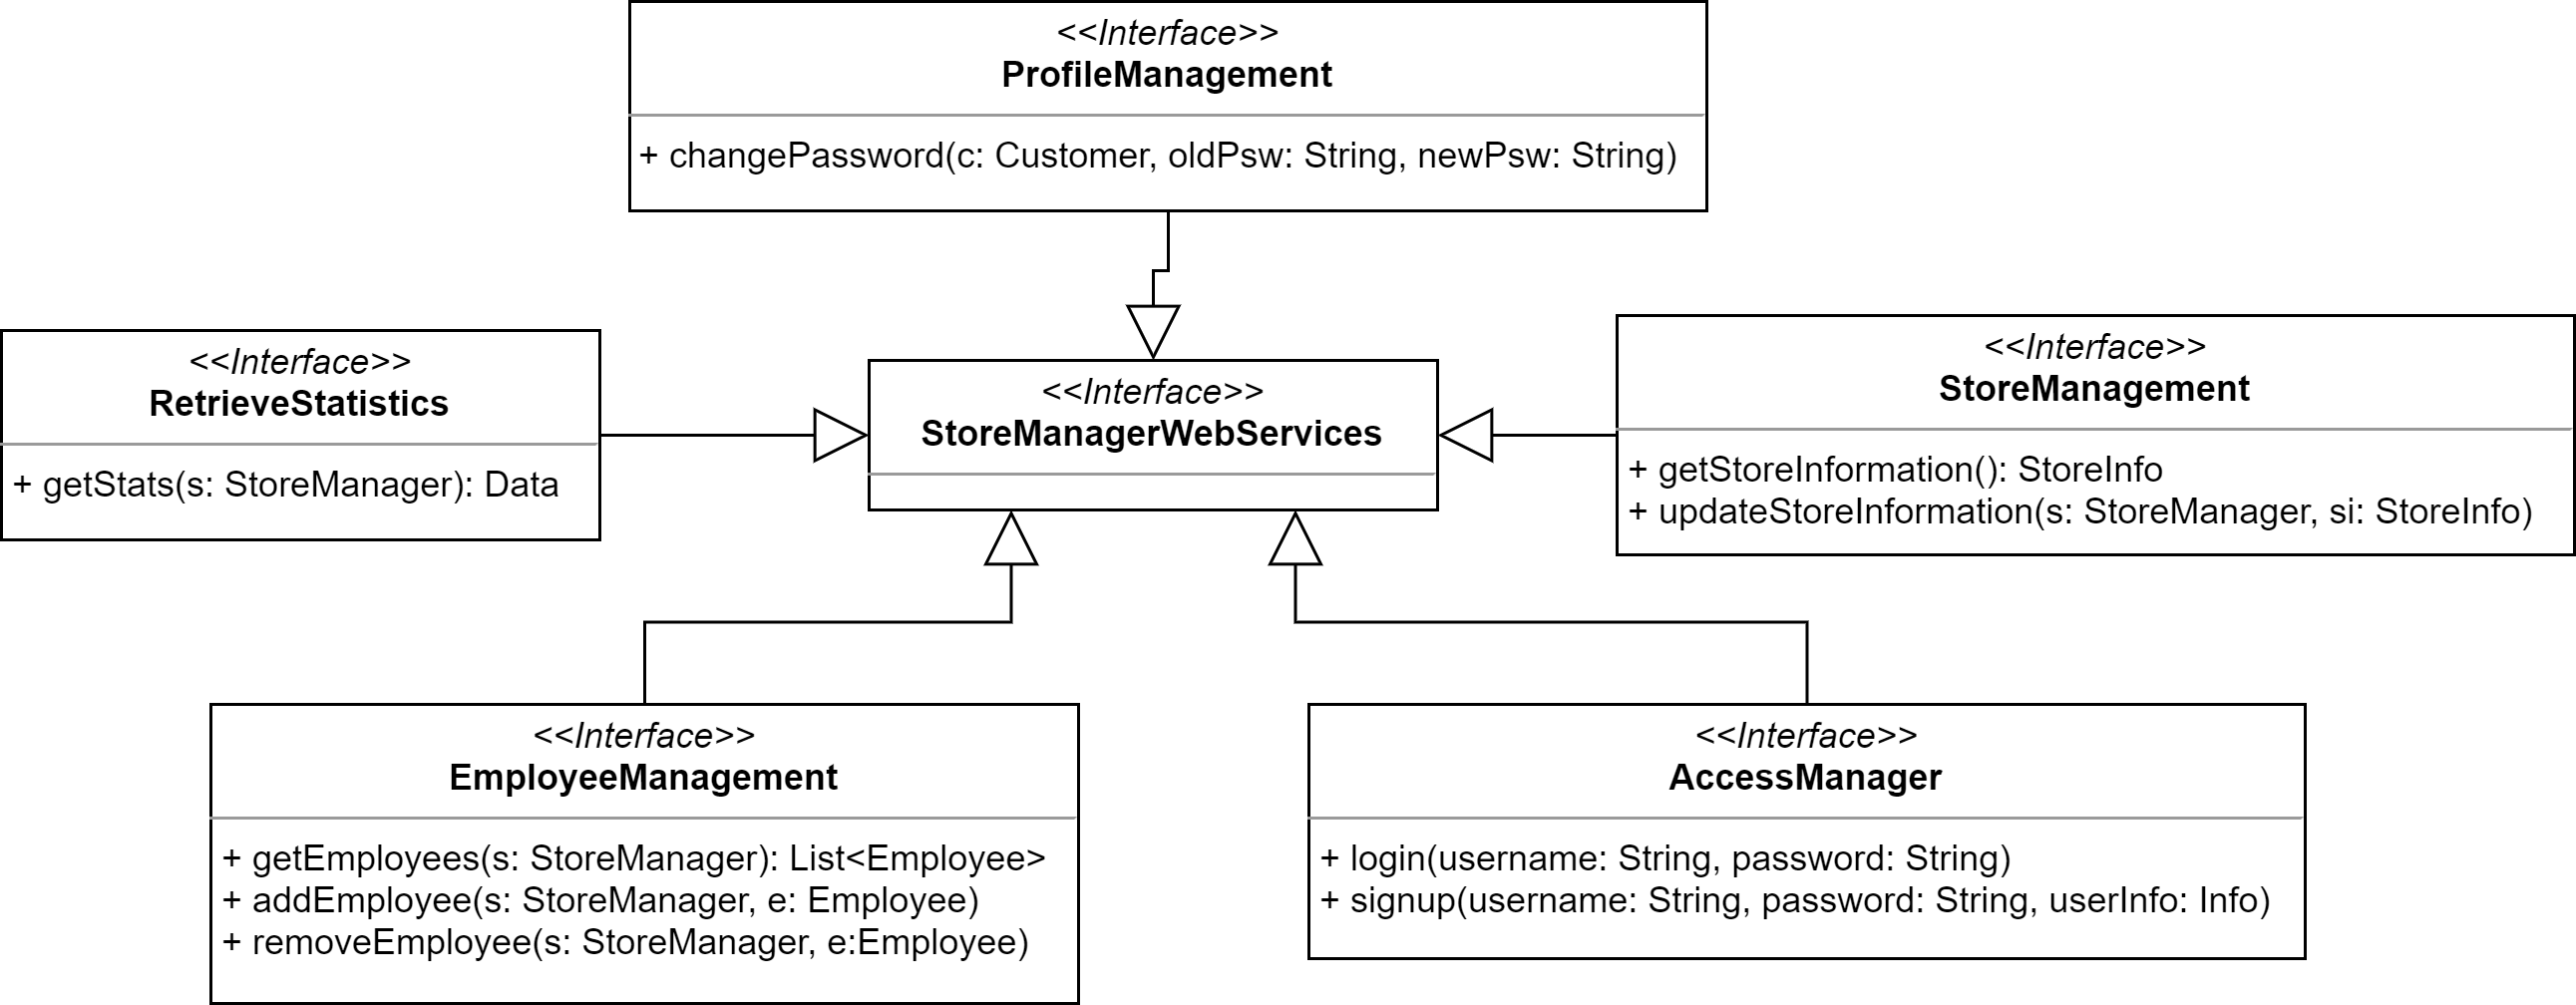
\includegraphics[width=16cm]{storeM_web_services_interfaces.png}
    \caption{Store Manager Web Services interfaces}
\end{figure}

	\section{Selected architectural styles and patterns}

		\subsection{Architectural styles}
In the overview section (2.1) there is a description of how a \textbf{three-tier client-server} architecture has been used to design the system. This choice favors, first of all, a greater decoupling of the system, increasing reusability, scalability and
flexibility. 

Regarding the transport protocol adopted, our choice is \textbf{HTTPS}. It's the secure version of HTTP, which is the primary protocol used to send data between the web browser and a website (like the web app used by Employees and the Store Manager). HTTPS is encrypted to increase the security of data transfer. This is particularly important when users transmit sensitive data, such as by logging into their account.

For the communication between the application and the system, our choice is a \textbf{REST} architecture. The goal was to reduce the coupling between client and server components. It fits very well for the scope because the goal is to update the server-side regularly, without touching the client software. This choice introduces the following constraints:
\begin{itemize}
    \item Layered Architecture
    \item Client-Server
    \item Stateless system
    \item Cacheable
\end{itemize}
All these constraints are respected by the choices previously made.

\subsection{Patterns}
    Selected design patterns:
    \begin{itemize}
        \item \textbf{Facade pattern} simplifies a complicated system by providing a single interface to a set of interfaces within a subsystem. It is used for some components designed in the component diagram in section 2.2.
    \end{itemize}
    Recommended architectural patterns for implementation:
    \begin{itemize}
        \item \textbf{Model-View-Controller pattern} is an architectural pattern that divides a given software application into three interconnected parts. This is done to separate internal representations of information from the ways information is presented to and accepted by the user. MVC is recommended because it is the best design pattern to structure our three-tier client-server architecture presented in the previous sections and it is one of the most common and effective ways to avoid a dangerous level of coupling between the various parts of the whole system.
    \end{itemize}
    Recommended design patterns for implementation:
    \begin{itemize}
        \item \textbf{Observer pattern} allows you to notify one or more objects about changes in the state of other objects within the system. It is recommended because it is essential to the previously recommended MVC model and is also useful in other CLup system applications.
        \item \textbf{Visitor pattern} is a way of separating an algorithm from an object structure on which it operates. A practical result of this separation is the ability to add new operations to existing object structures without modifying the structures. It decoupling the operations from the object structure. This pattern is useful for the MVC application too.
        \item \textbf{Factory pattern} is a creational pattern that uses factory methods to deal with the problem of creating objects without having to specify the exact class of the object that will be created. It is particularly useful if applied in combination with the MVC pattern.
    \end{itemize}


	\section{Other design decisions}

		\textbf{Maps APIs:}
to calculate the estimated time to reach the store, a public maps service is necessary. The Google Maps APIs are a good choice to do that. In particular, the Routes service will be used to estimate the travel time from the customer to the grocery shop.

\bigbreak
\textbf{Notifications APIs:}
to deliver notifications to customers about their position in the queue Firebase Cloud Messaging may be used. Firebase is easy to integrate with the Flutter framework and provides an easy set-up to send push notifications to both iOS and Android clients.

\chapter{User Interface Design}\label{chapt:sum}

		In addition to the views provided in the RASD document, in the next few pages we are going to present additional mockups which will give a complete overview of how the application and the web application will look like.

\begin{figure}[H]
    \begin{minipage}[b]{8cm}
    \centering
    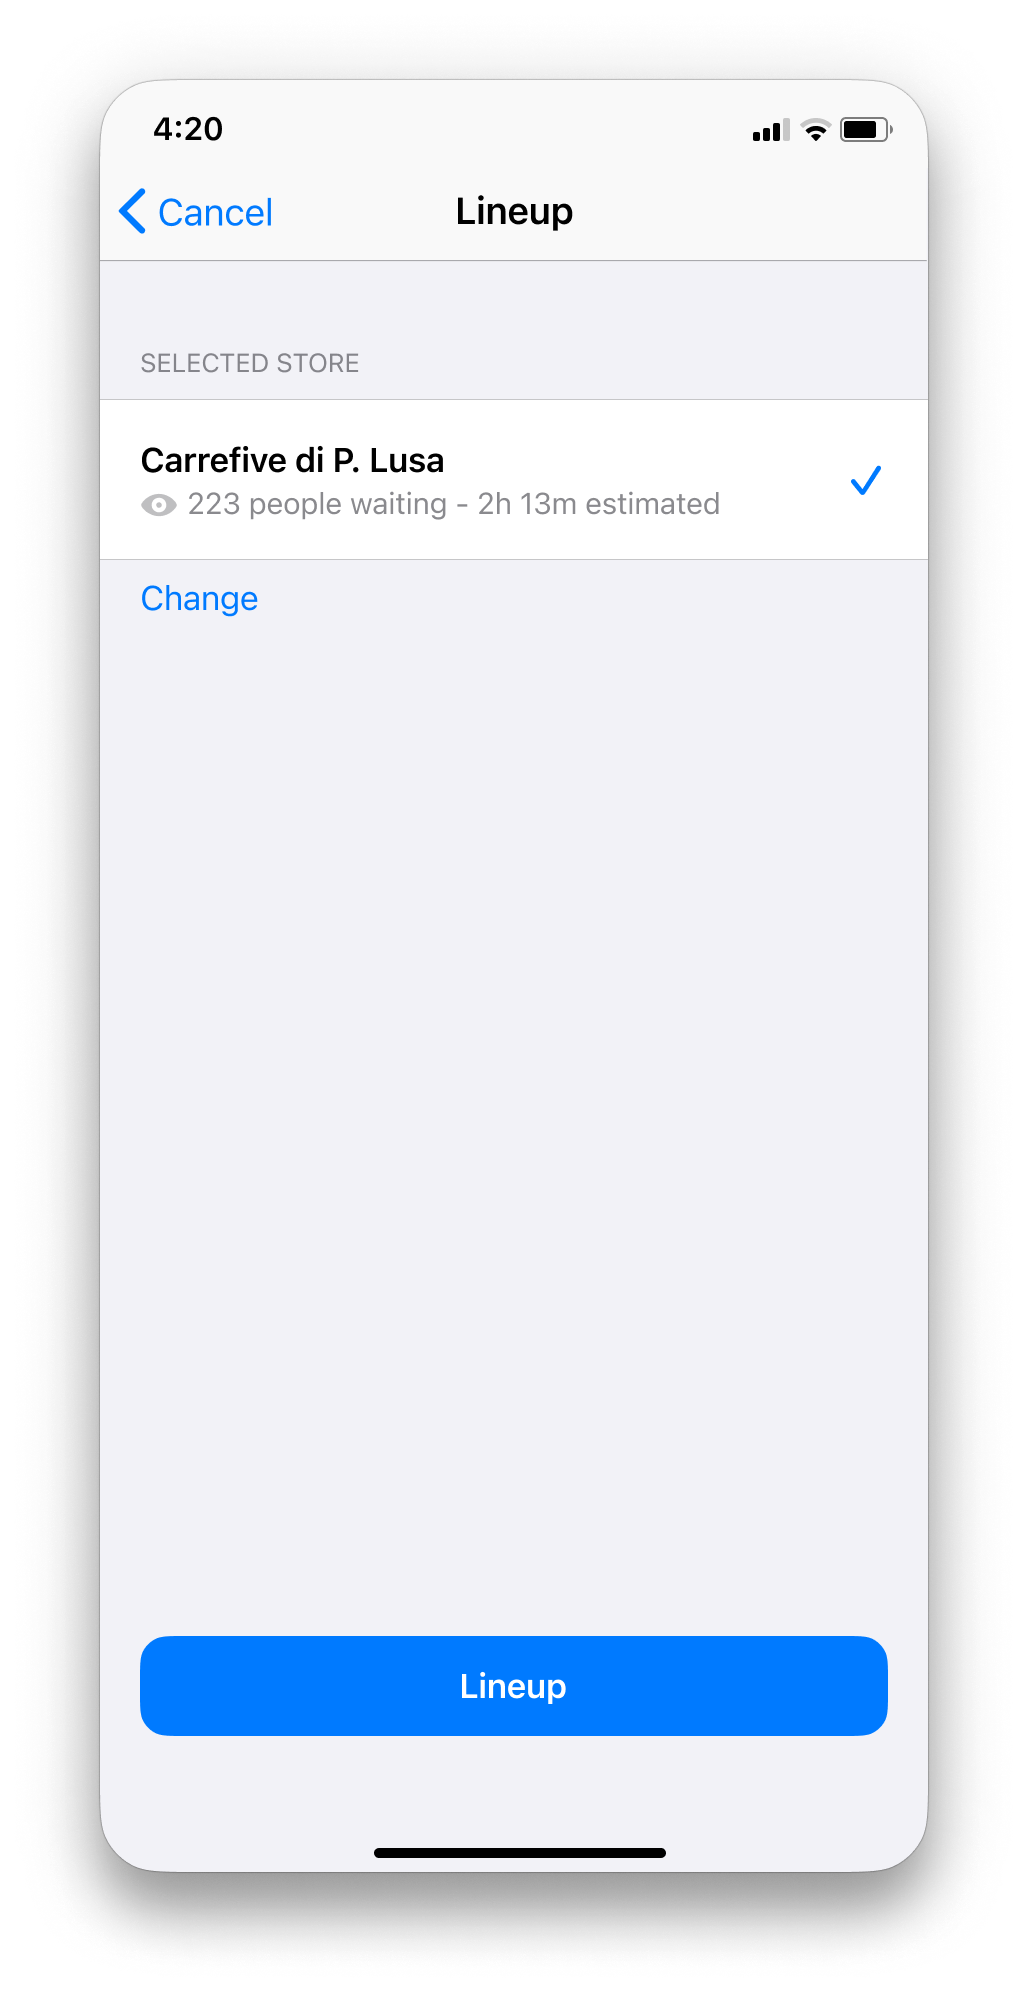
\includegraphics[width=6cm]{AppNewLineup.png}
    \caption{Lineup page}
    \end{minipage}
    \ \hspace{2mm} \hspace{3mm} \
    \begin{minipage}[b]{8cm}
    \centering
    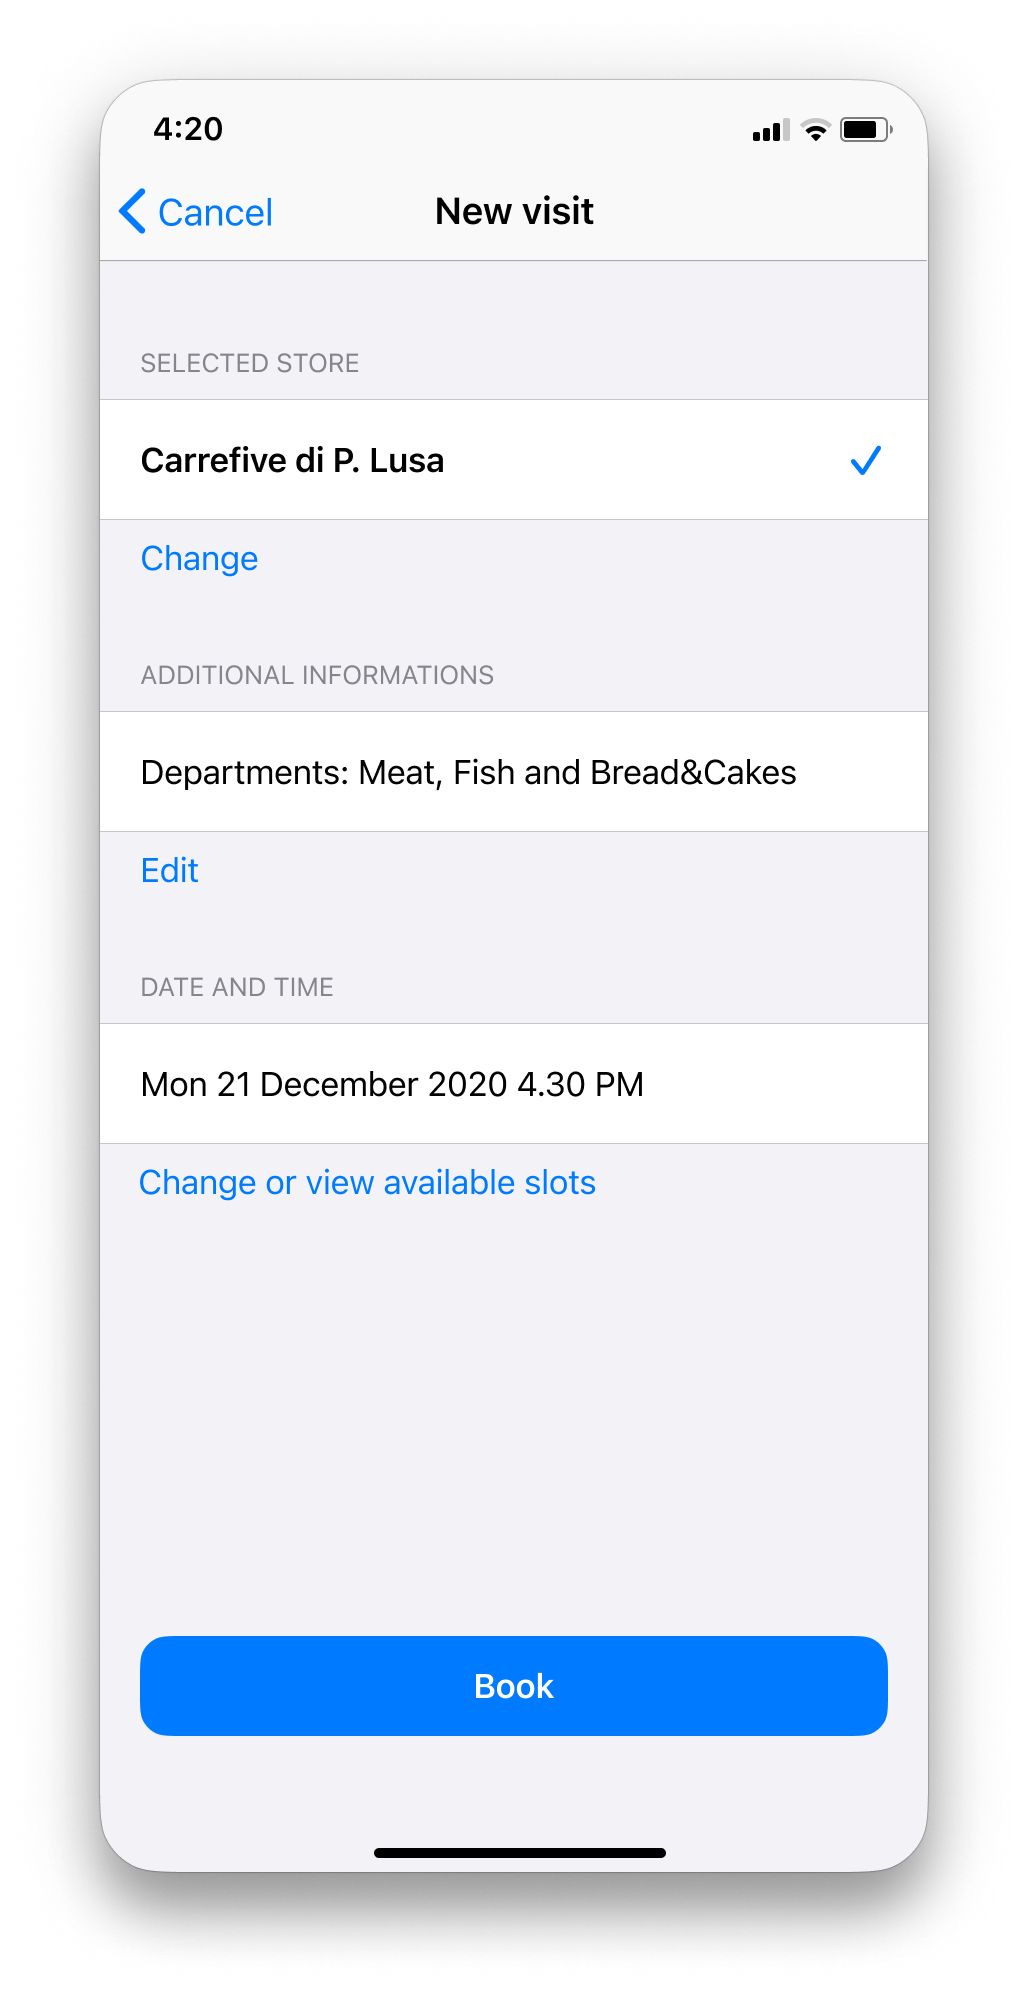
\includegraphics[width=6cm]{AppNewVisit.png}
    \caption{Book a visit}
    \end{minipage}
\end{figure}

\begin{figure}[H]
    \begin{minipage}[b]{8cm}
    \centering
    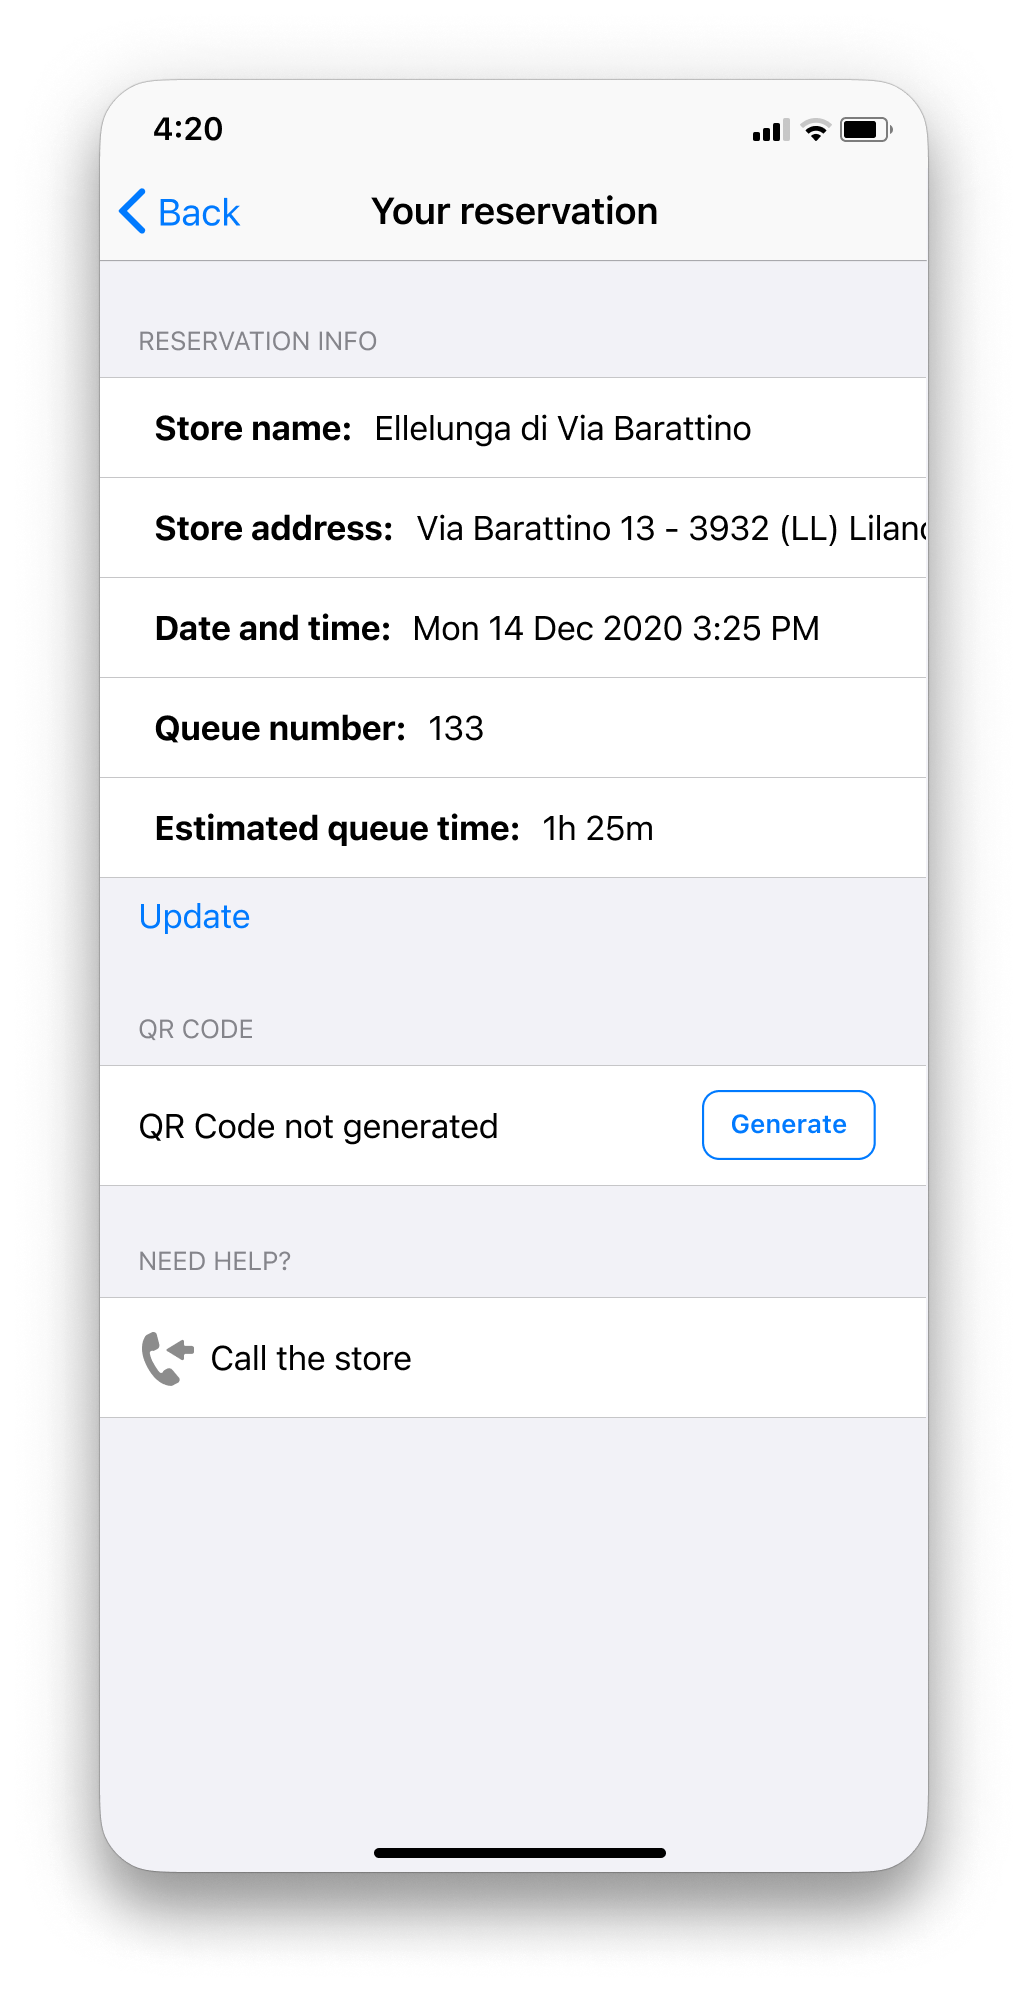
\includegraphics[width=6cm]{AppReservationDetails.png}
    \caption{Reservation details}
    \end{minipage}
    \ \hspace{2mm} \hspace{3mm} \
    \begin{minipage}[b]{8cm}
    \centering
    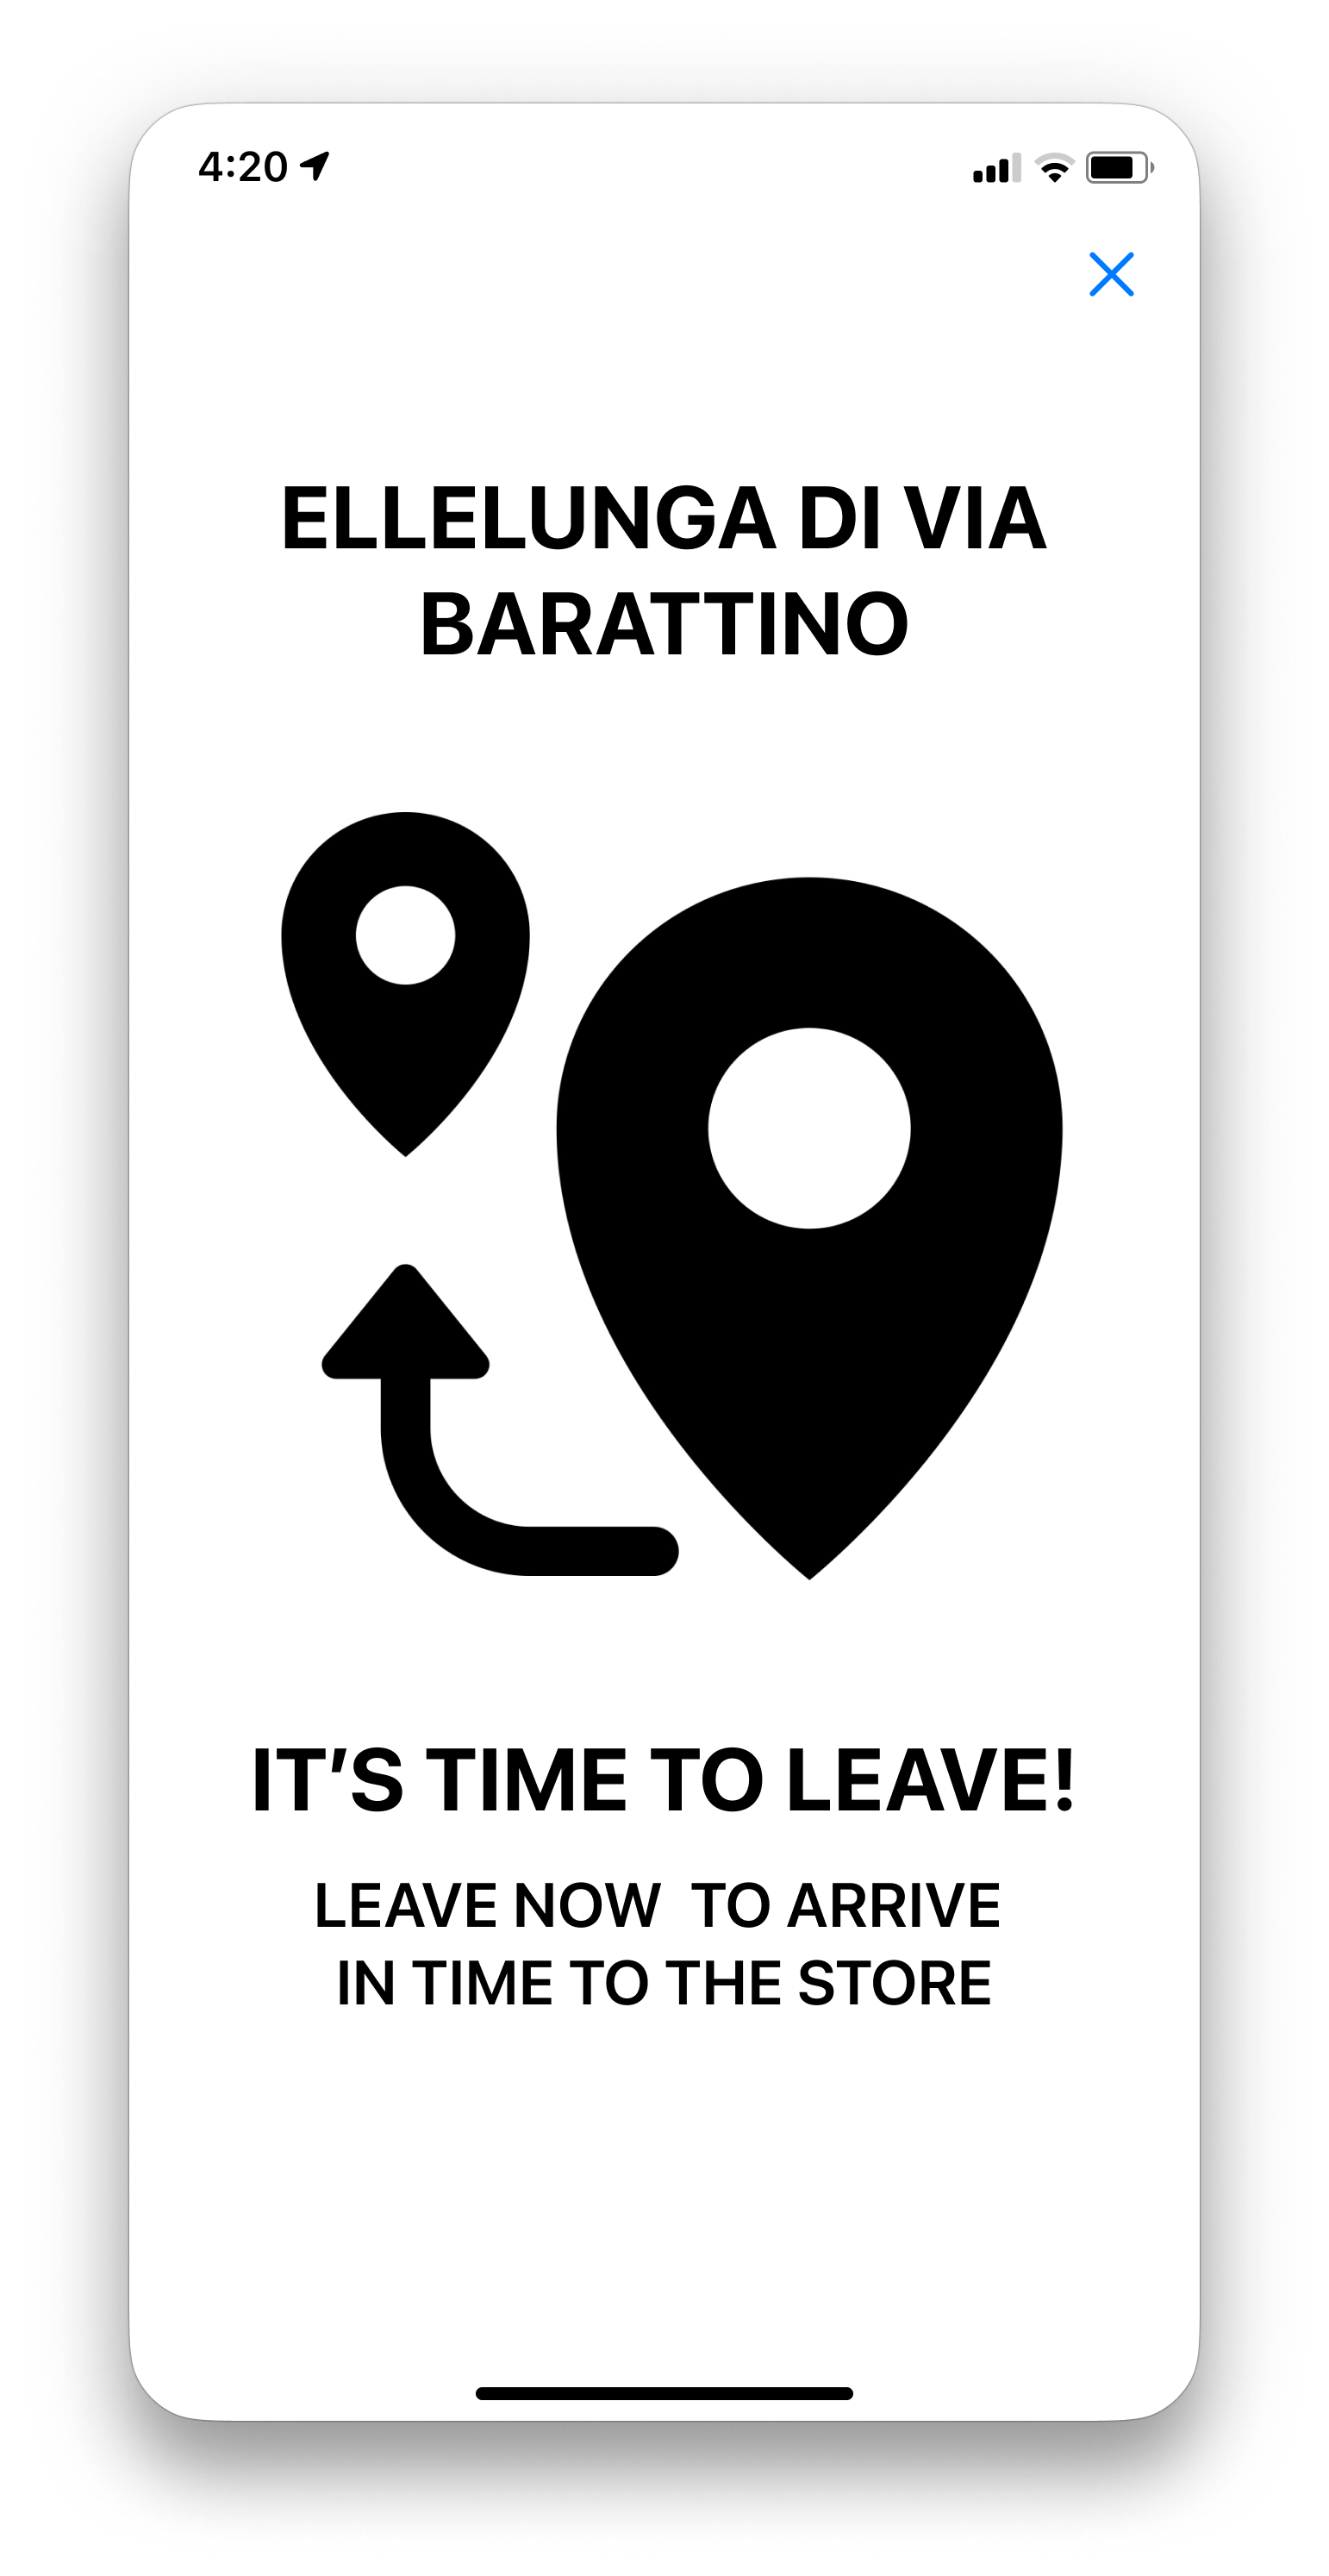
\includegraphics[width=6cm]{AppCall.png}
    \caption{Notification}
    \end{minipage}
\end{figure}

\begin{figure}[H]
    \centering
    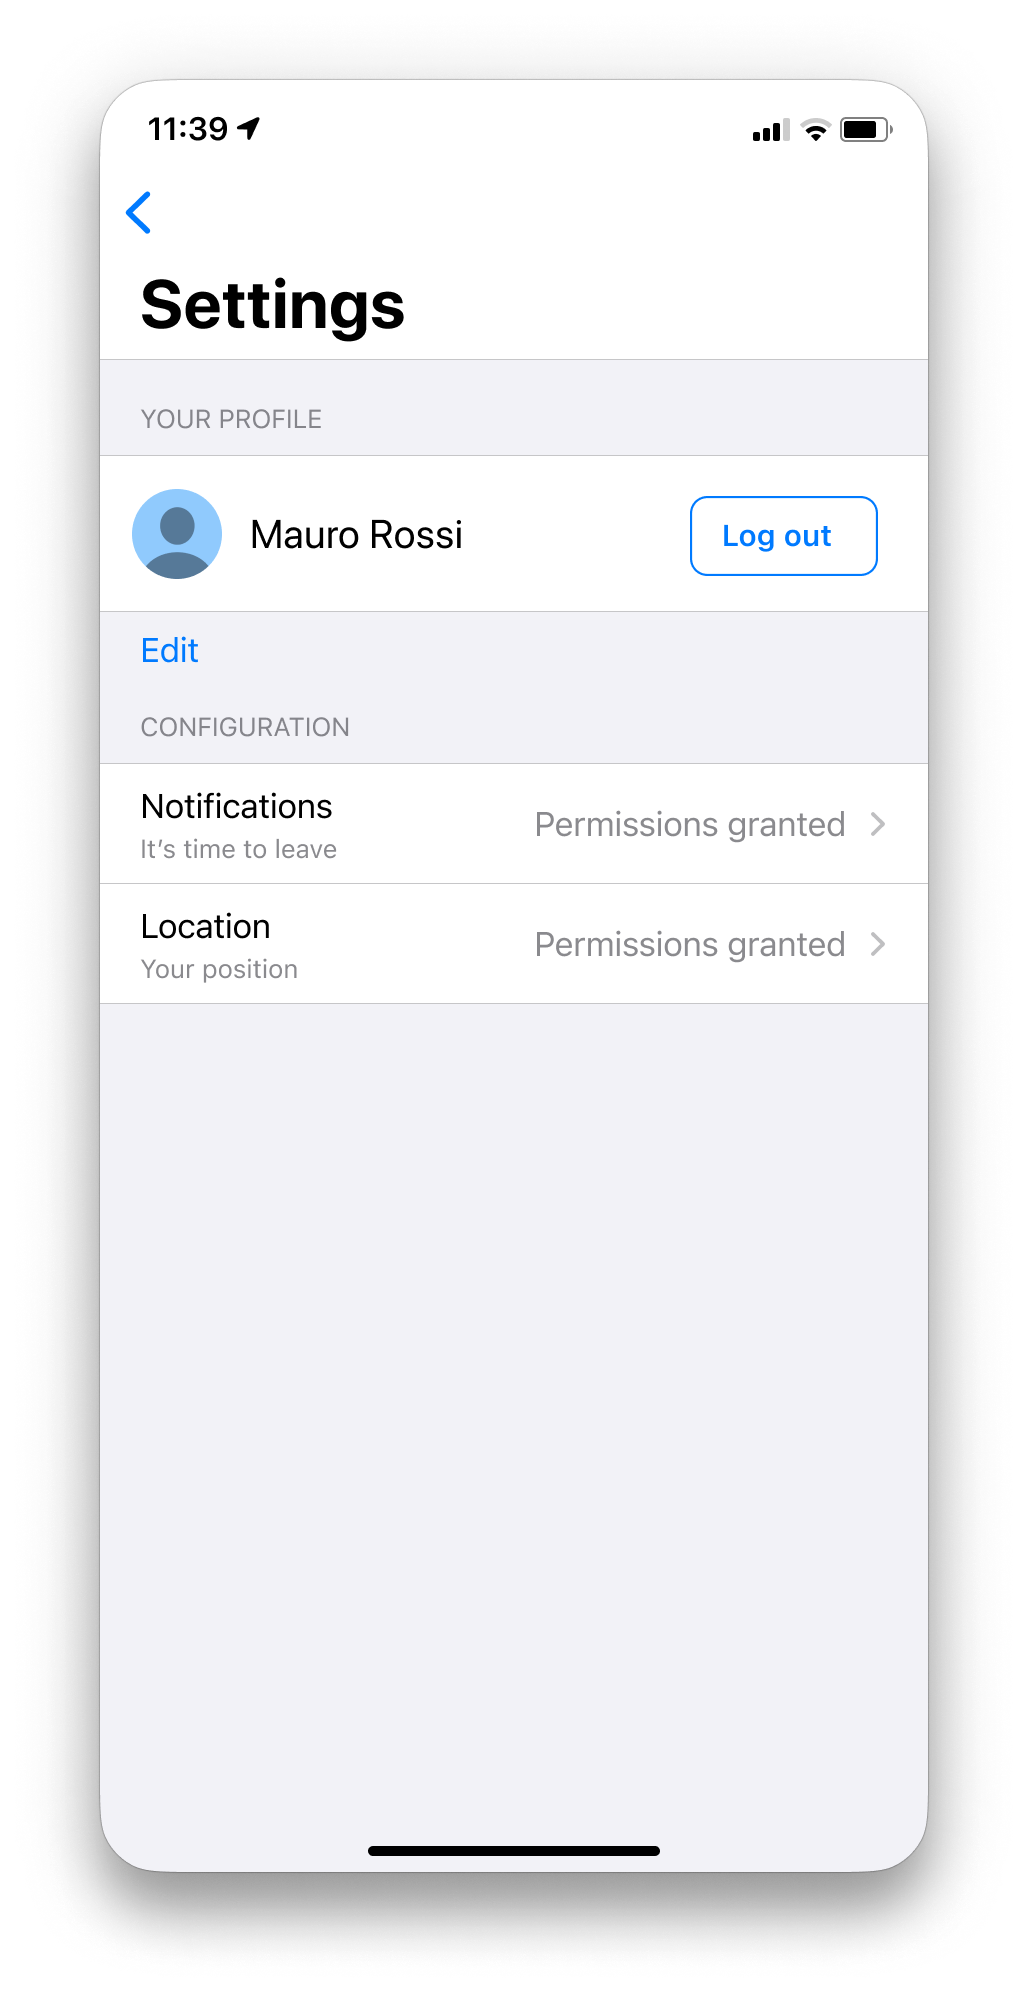
\includegraphics[width=6cm]{AppSettings.png}
    \caption{Settings}
\end{figure}

\begin{figure}[H]
    \centering
    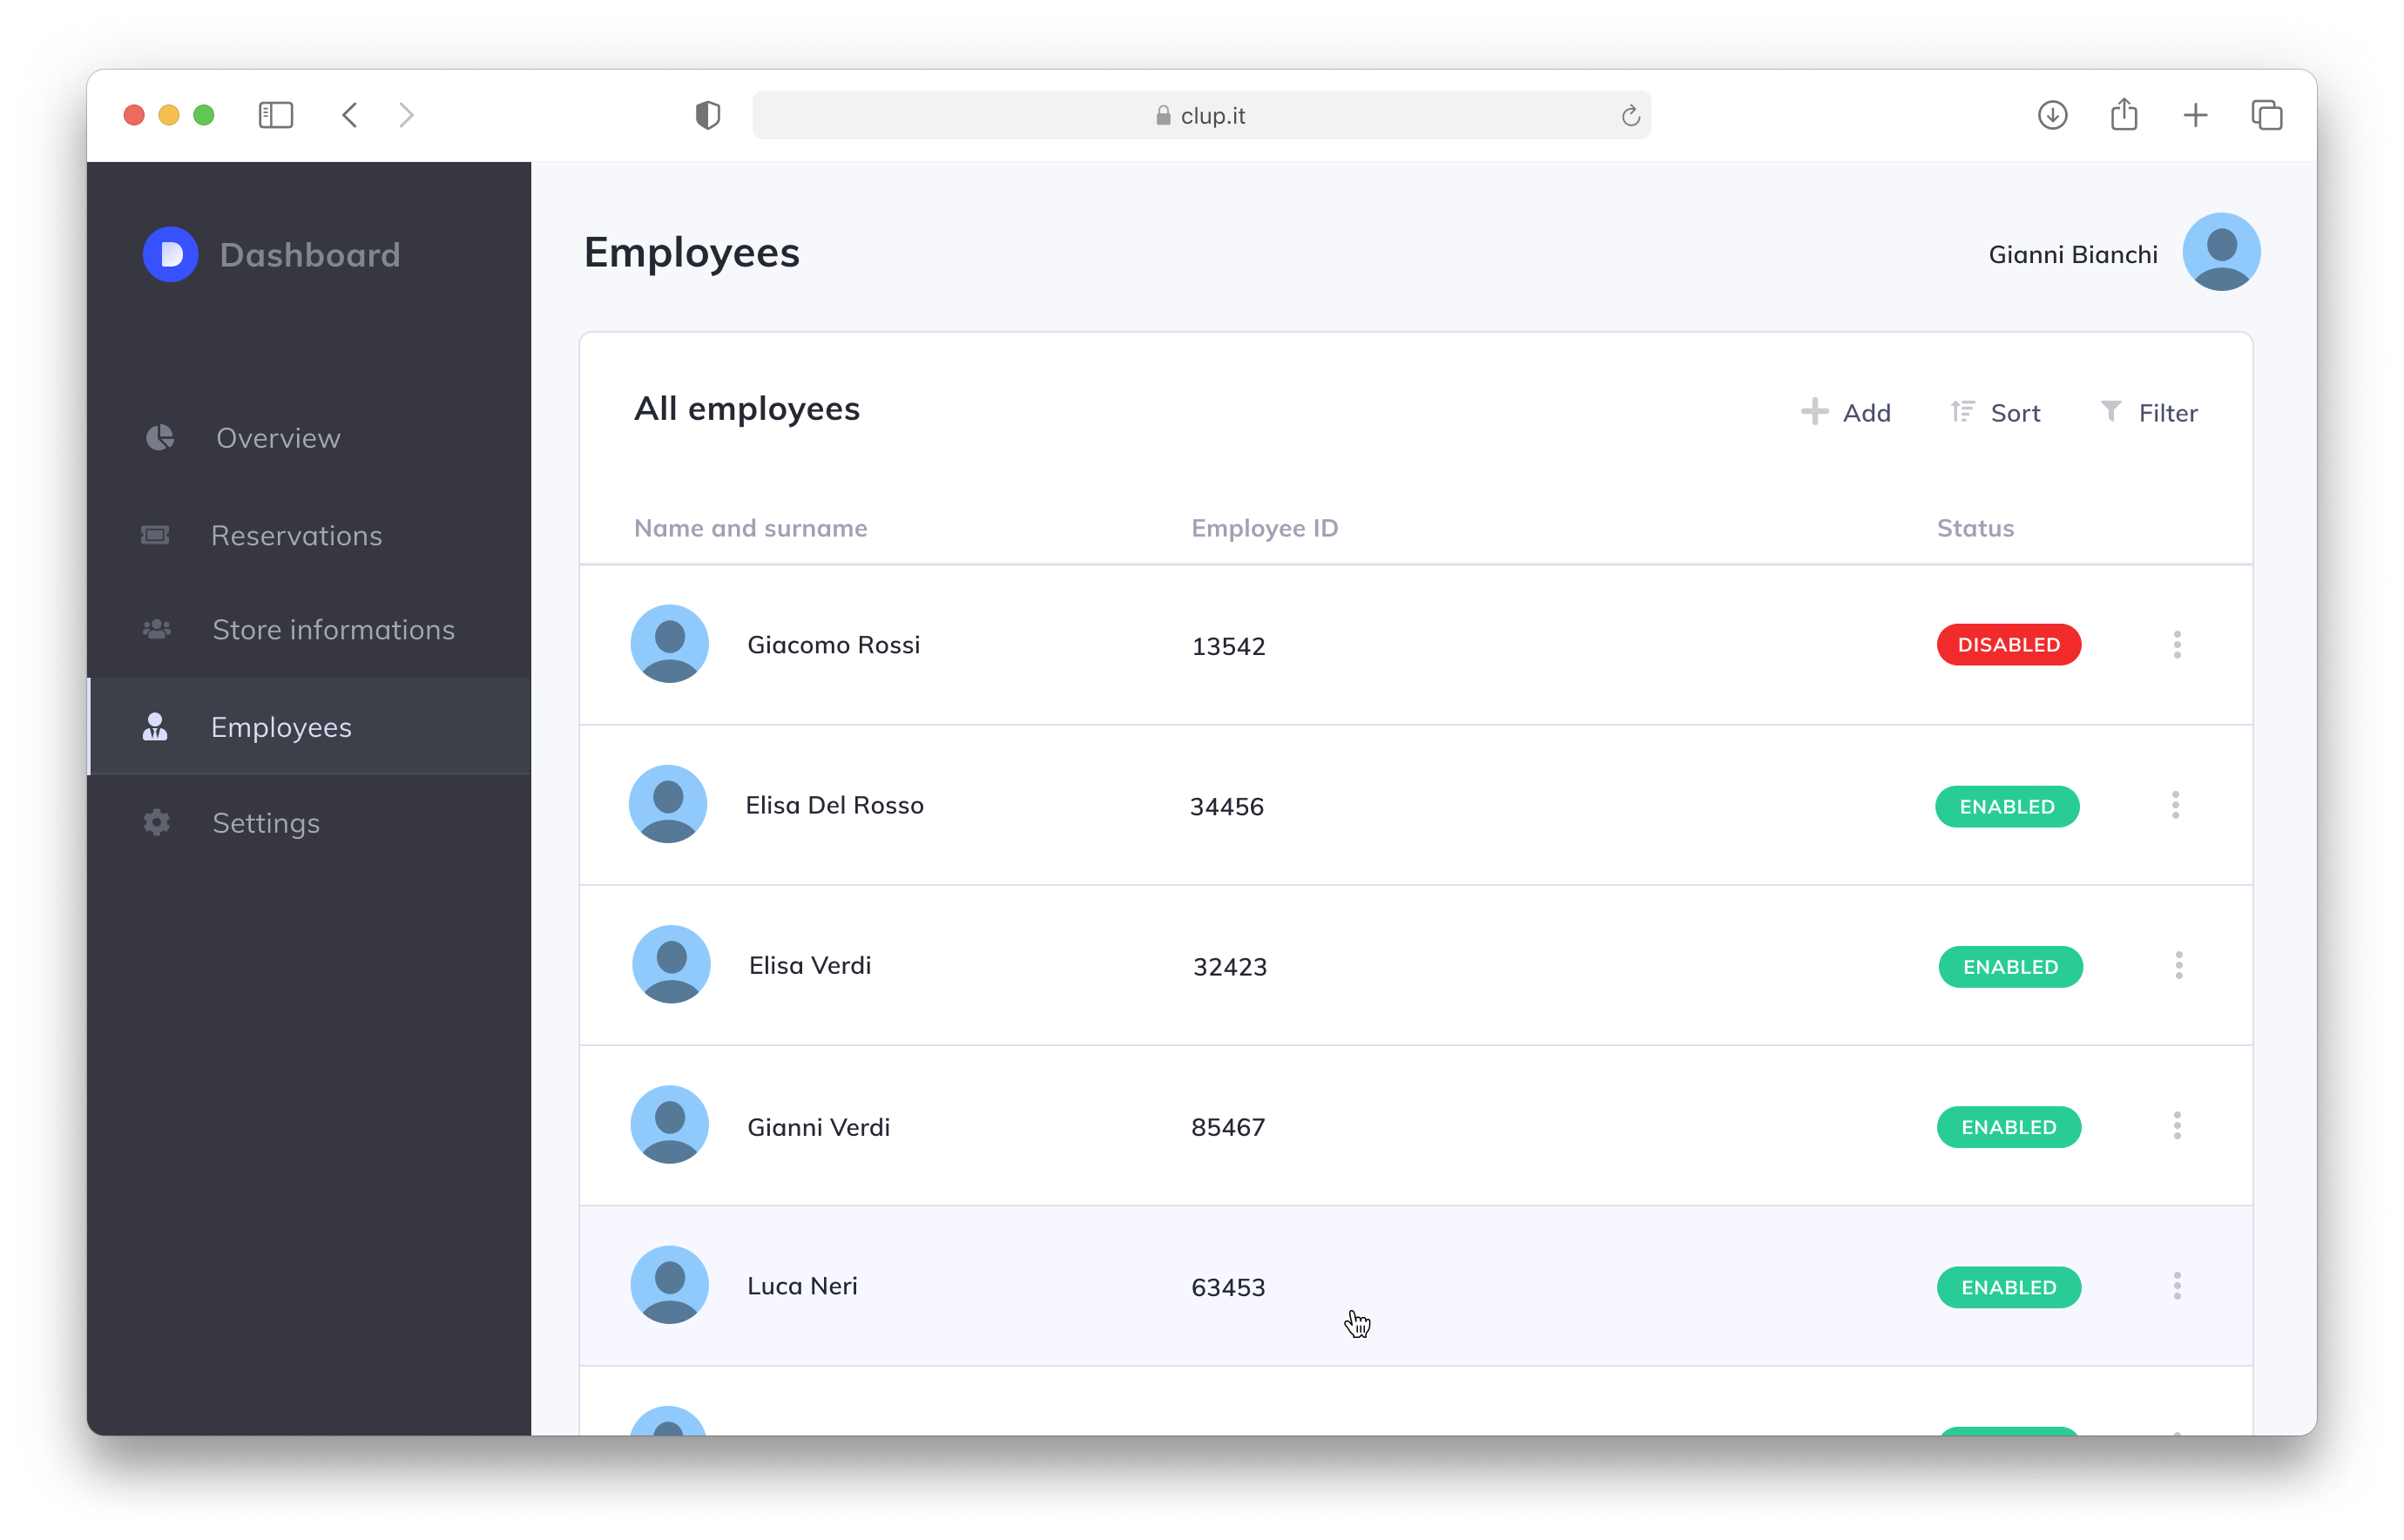
\includegraphics[width=16cm]{WebAppEmployees.png}
    \caption{Employees page}
\end{figure}

\begin{figure}[H]
    \centering
    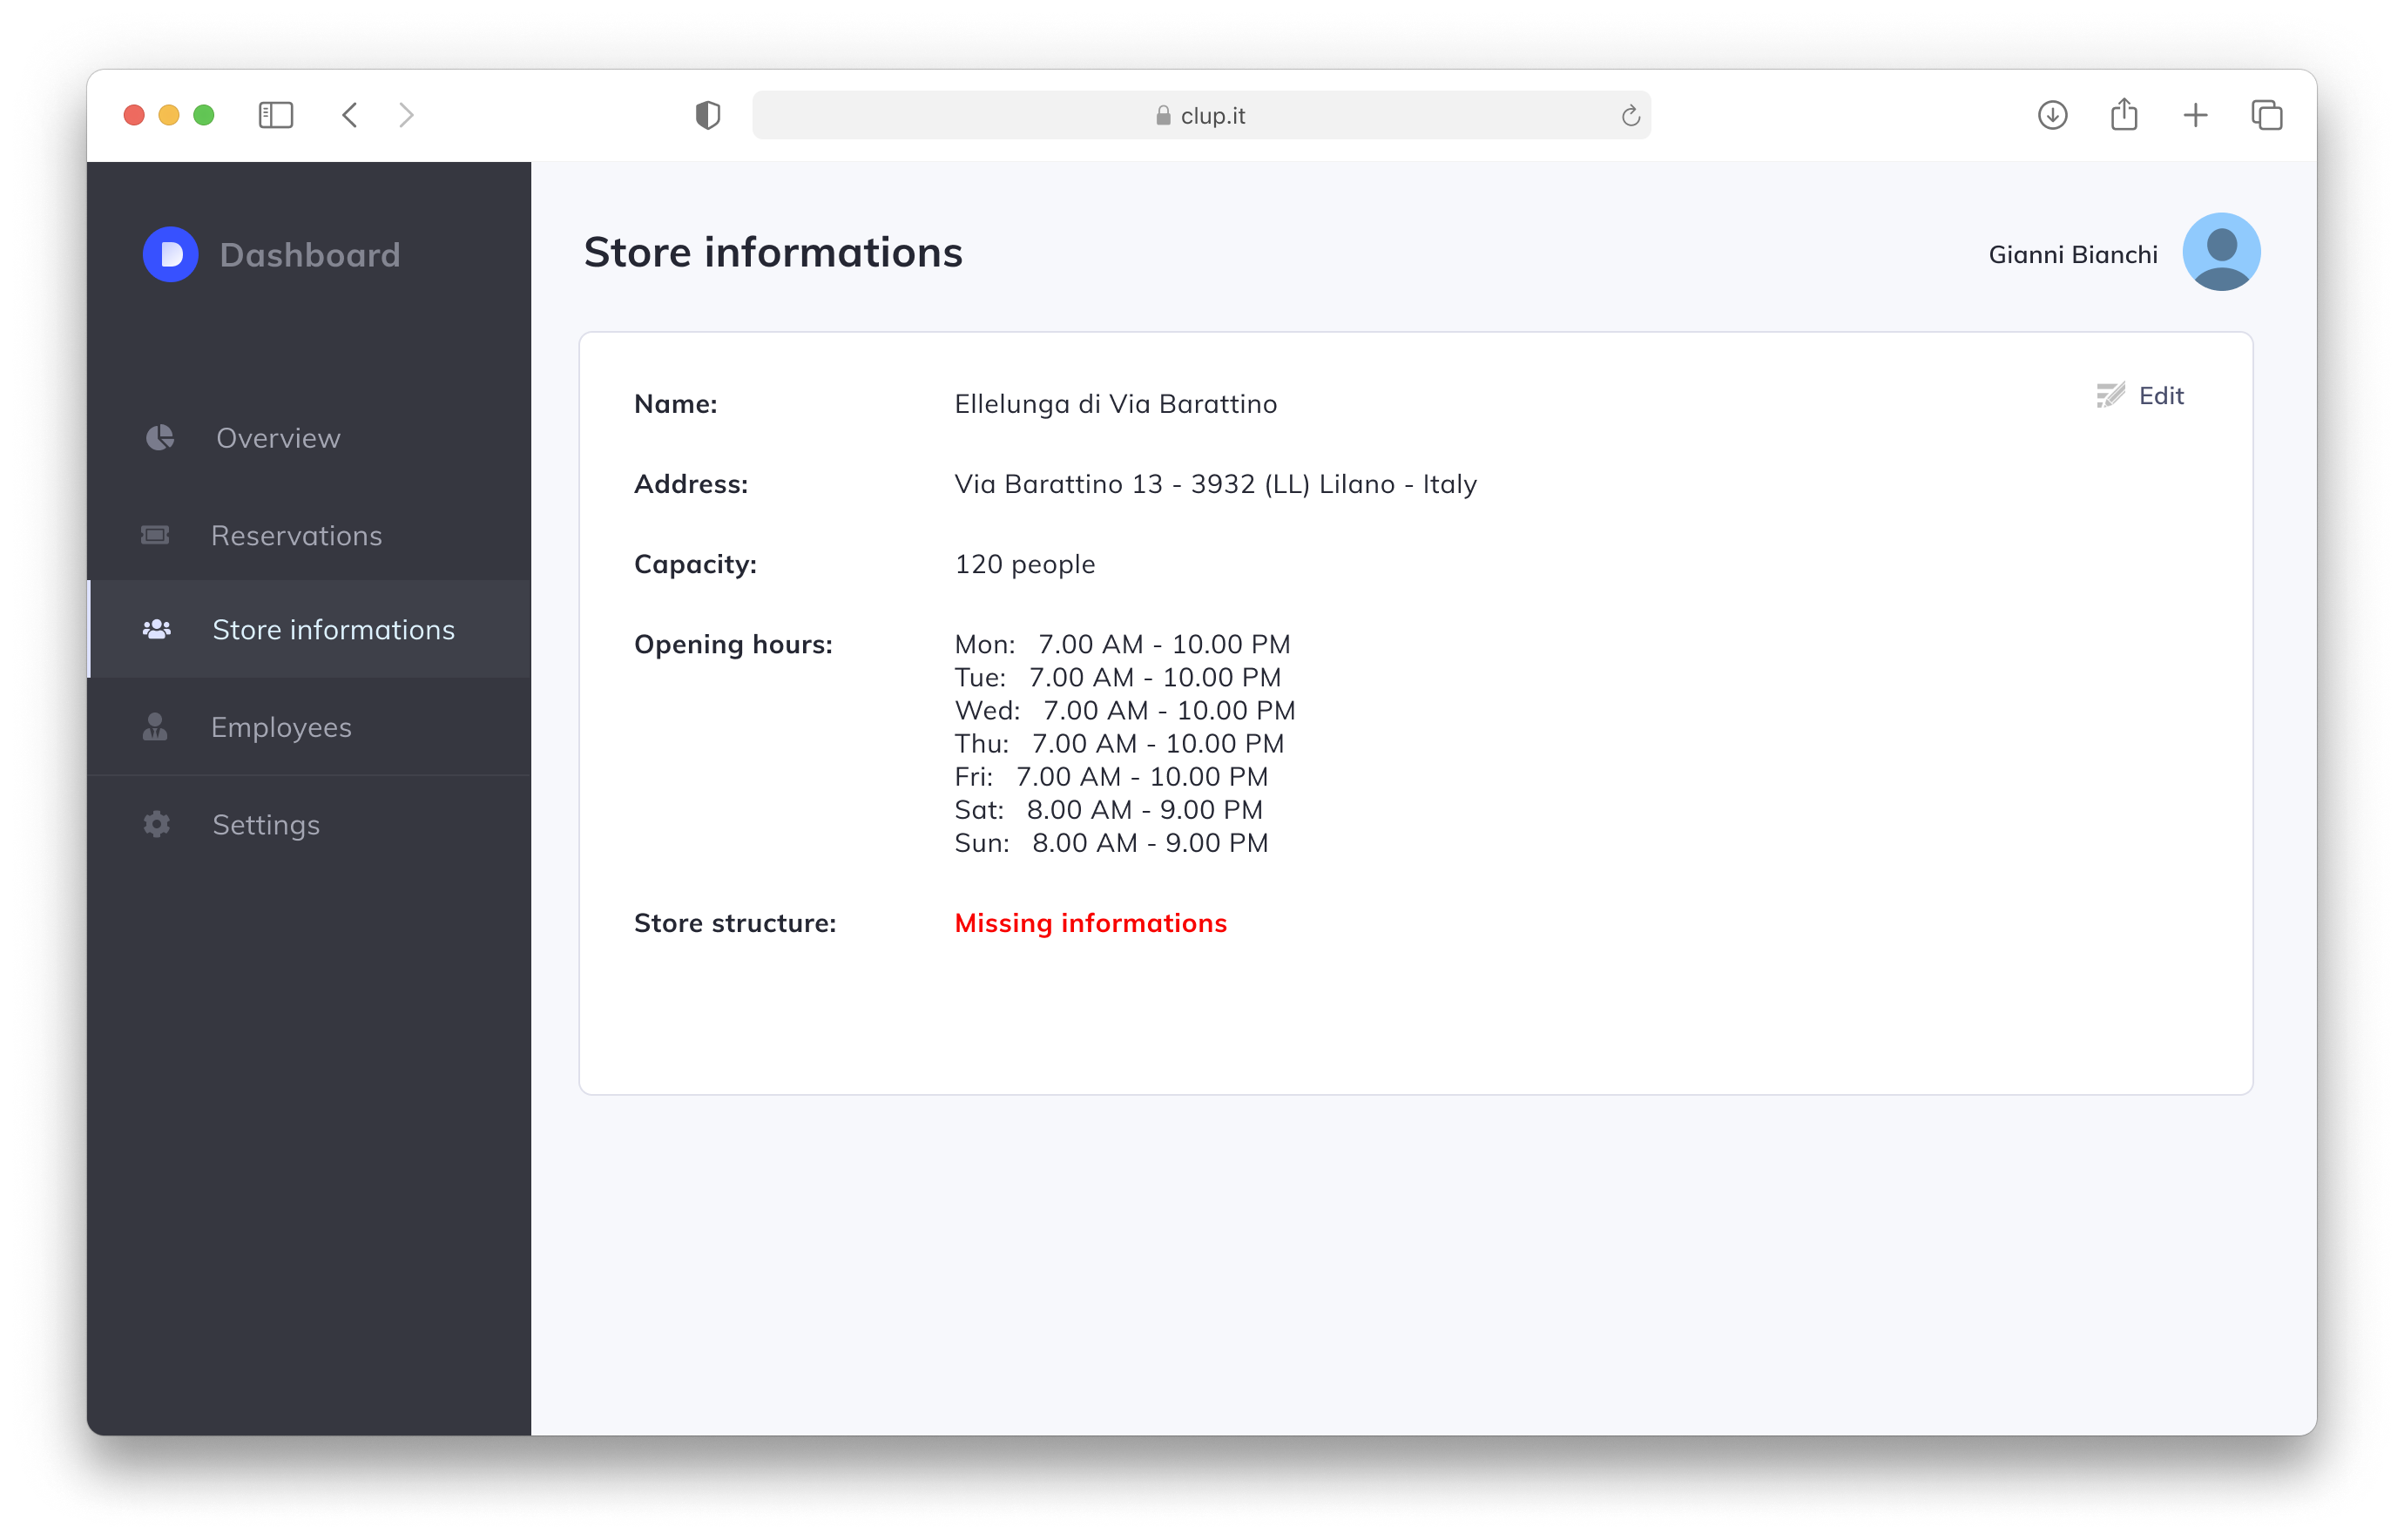
\includegraphics[width=16cm]{WebAppStoreInformations.png}
    \caption{Store informations}
\end{figure}

\begin{figure}[H]
    \centering
    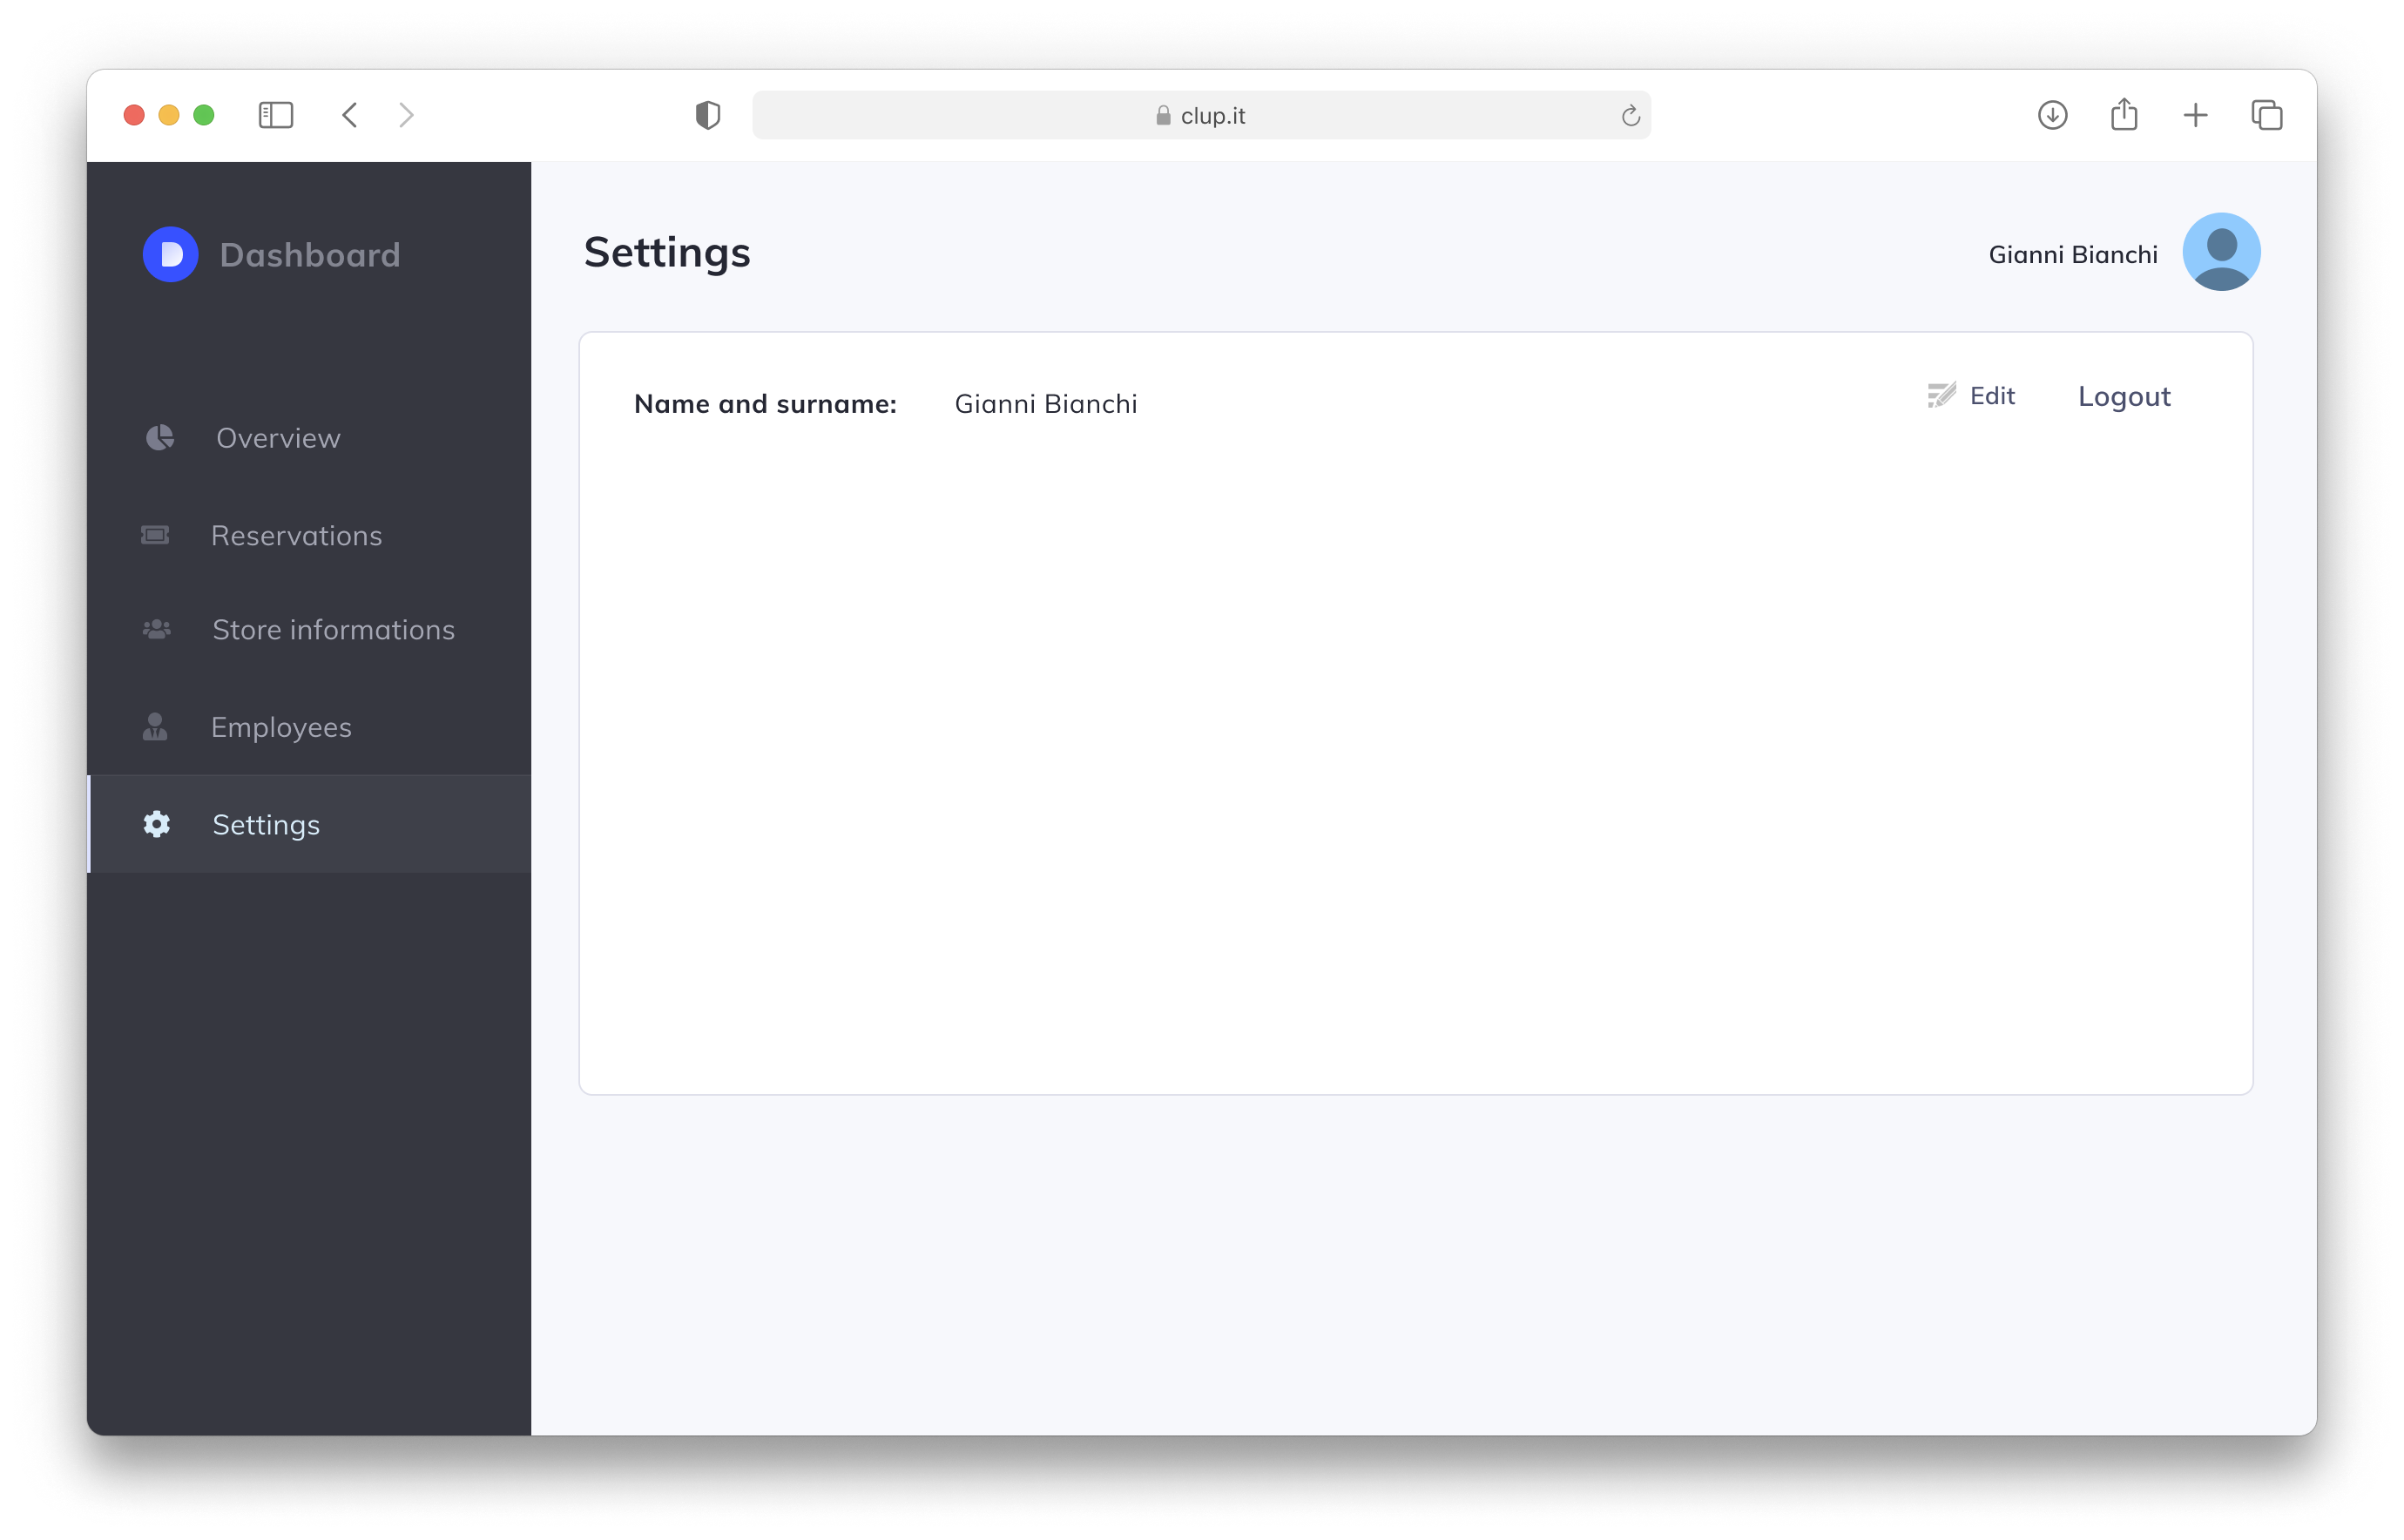
\includegraphics[width=16cm]{WebAppSettings.png}
    \caption{Settings}
\end{figure}

\begin{figure}[H]
    \centering
    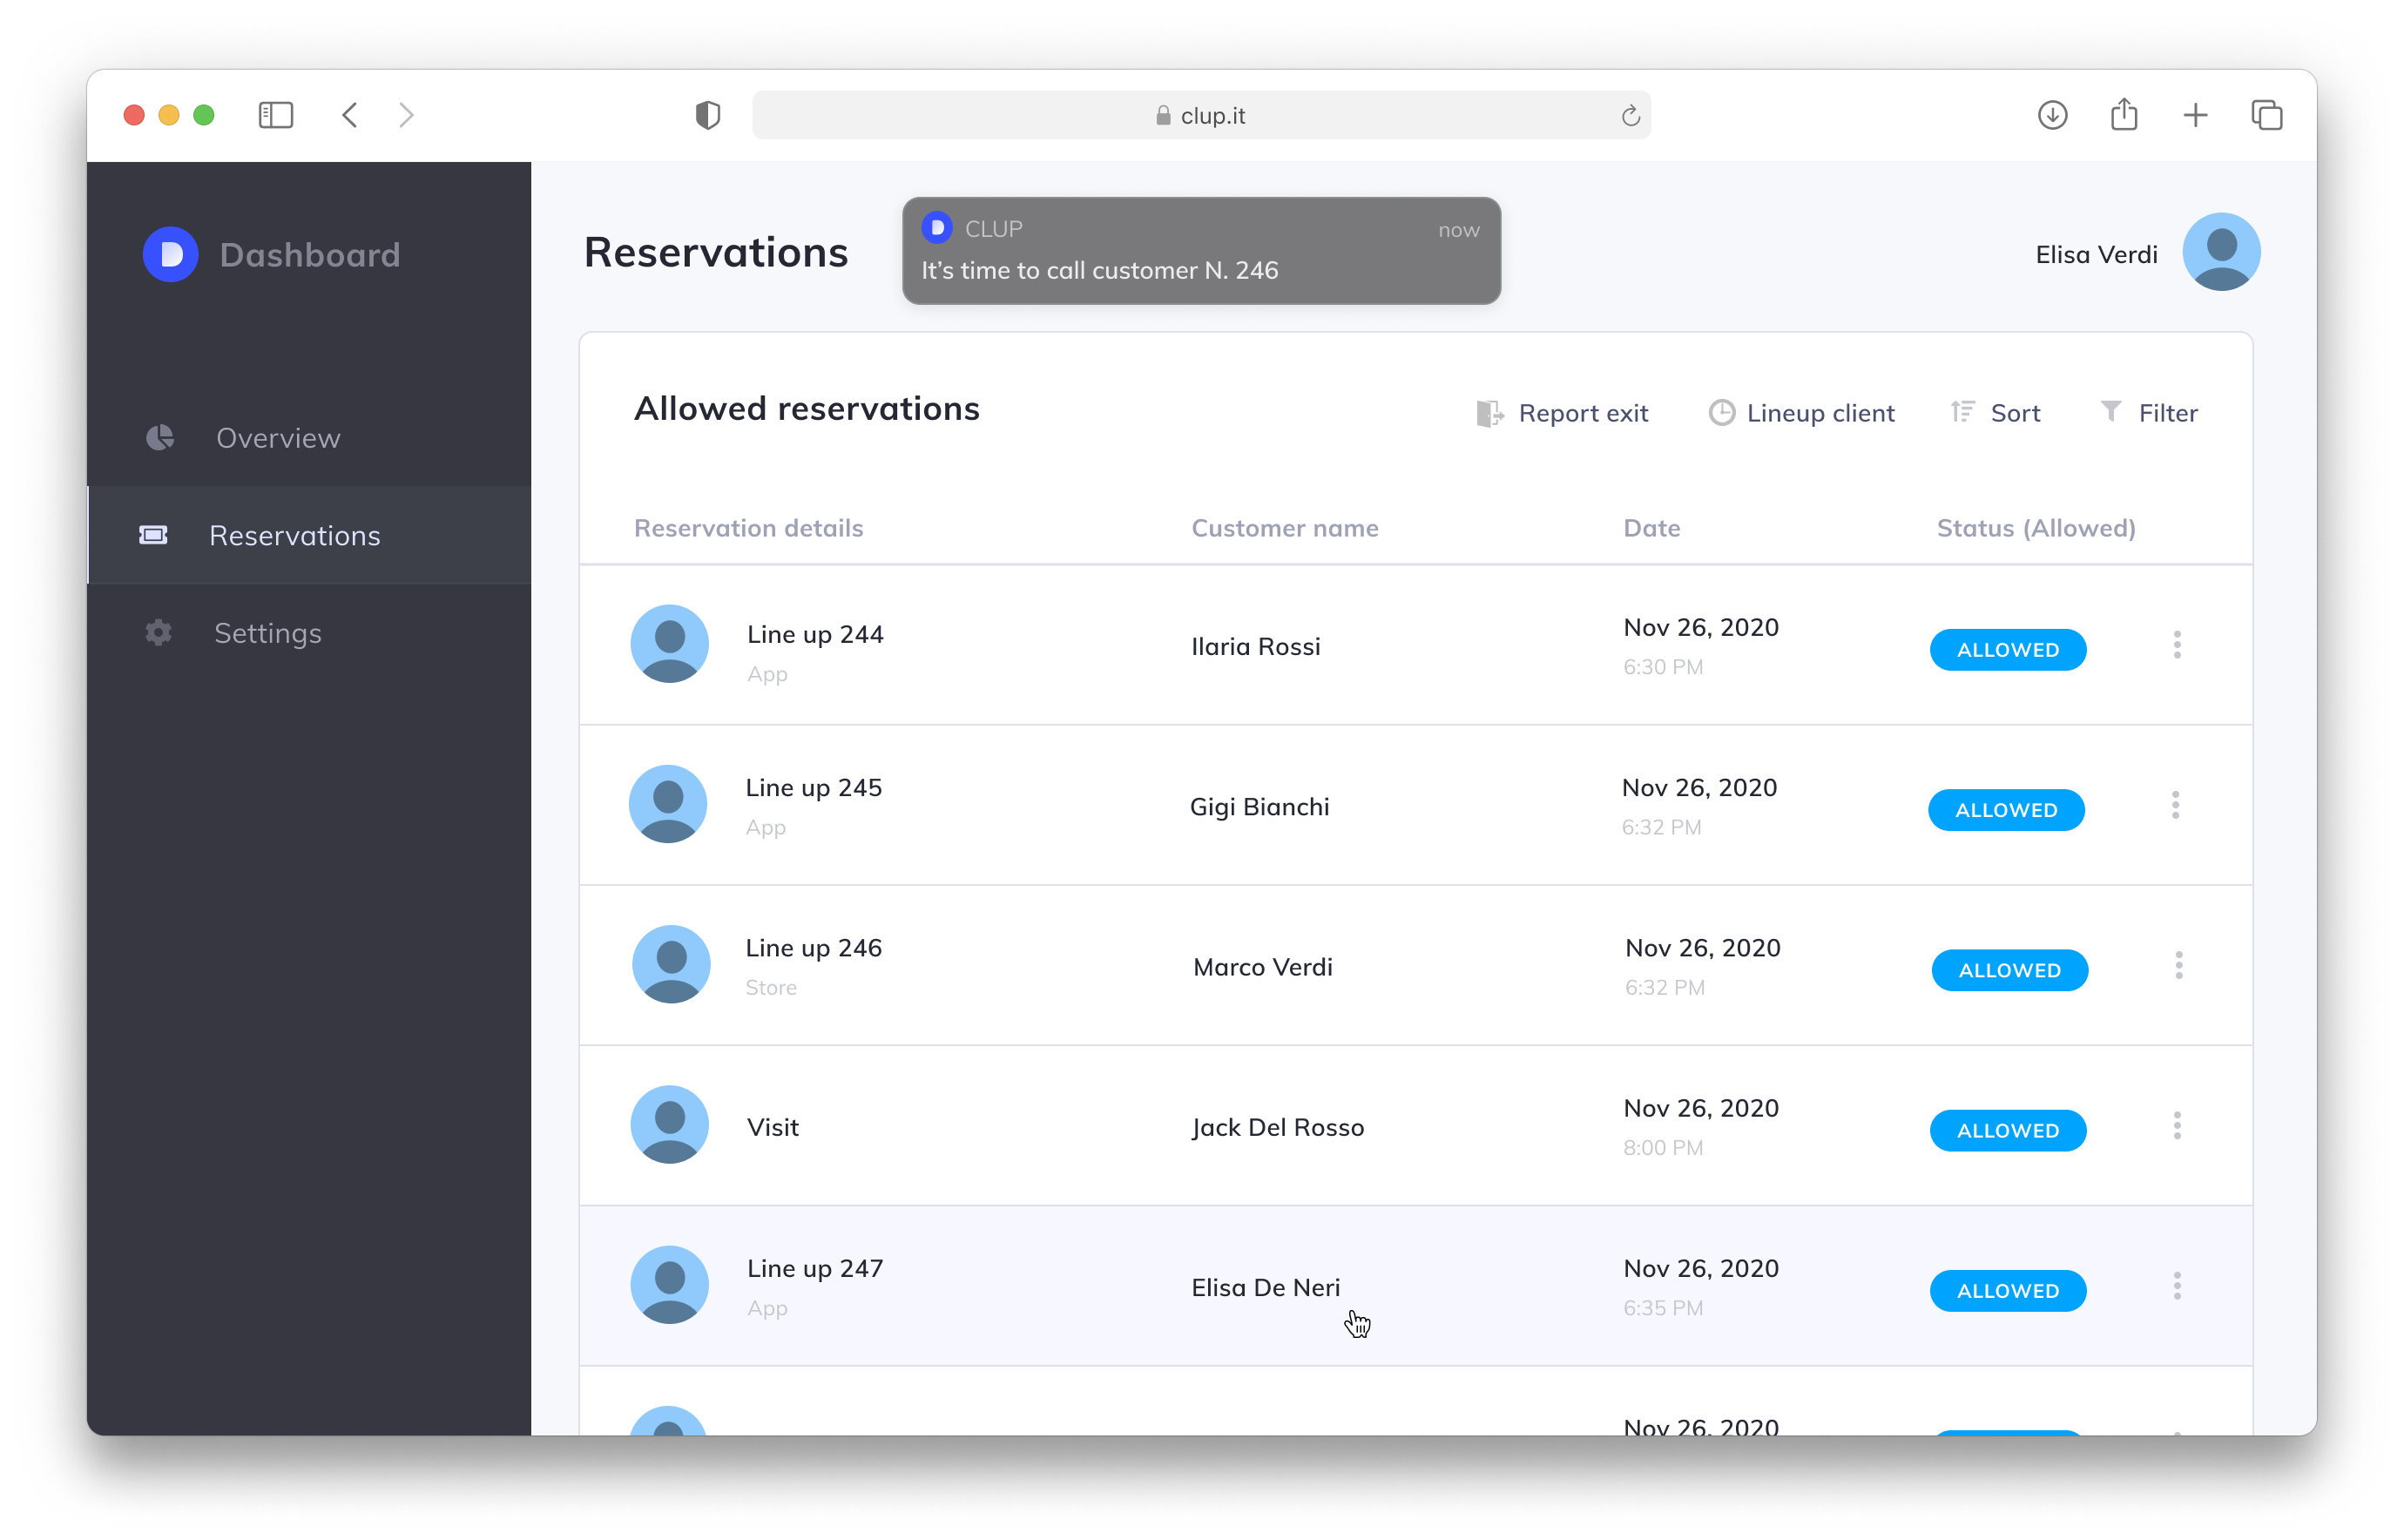
\includegraphics[width=16cm]{WebAppReservations(Employee).png}
    \caption{Reservation page (Employee view)}
\end{figure}

\chapter{Requirements Traceability}\label{chapt:sum}

	This chapter explains how to implement, integrate, and test the system designed in this document. We decided to explain this in 3 steps. The first one (\textbf{Implementation, Component Integration and Testing}) talks about how to implement the single component (the order), how to integrate and test them.
The second step (\textbf{System Testing}) explains the plan to test the system implemented. The last step (\textbf{Additional Specification on Testing}) gives additional information to make easier the testing process.

	\begin{center}
    {\renewcommand{\arraystretch}{1.5}
    \begin{longtable}{L{2.5cm}L{12cm}}
        \hline
        \rowcolor{shadeColorGoal}\textbf{G1} & \textbf{Everyone can use and interact with the CLup system accordingly with itsfeatures and processes} \\
        \hline
        \rowcolor{shadeColorRequirement} R1 & Visitors are allowed to register as customers through the CLup application \\
        \hline
        \rowcolor{shadeColorRequirement} R2 & The store manager is allowed to register as store manager through the CLup web app \\
        \hline
        \rowcolor{shadeColorRequirement} R3 & Customers are allowed to log in inside the application \\
        \hline
        \rowcolor{shadeColorRequirement} R4 & The store manager and the employee are allowed to login in inside the web application \\
        \hline
        \rowcolor{shadeColorRequirement} R6 & The store manager can create and edit the employees’ accounts associated to his/her store \\
        \hline
        \rowcolor{shadeColorComponents} & \textbf{Components} mapped to the above requirements:

        \medskip
        \medskip
        \begin{itemize}
            \item Customer Mobile Services \begin{itemize}
                \item AccountManager
            \end{itemize}
            \item Employee Web Services \begin{itemize}
                \item AccountManager
            \end{itemize}
            \item Store Manager Web Services \begin{itemize}
                \item AccountManager
                \item StoreInfoAndEmployeesManager
            \end{itemize}
        \end{itemize} \\
        \hline
    \end{longtable}}

    {\renewcommand{\arraystretch}{1.5}
    \begin{longtable}{L{2.5cm}L{12cm}}
        \hline
        \rowcolor{shadeColorGoal}\textbf{G2} & \textbf{All customers who reserve a place in the queue will be called} \\
        \hline
        \rowcolor{shadeColorRequirement} R3 & Customers are allowed to log in inside the application \\
        \hline
        \rowcolor{shadeColorRequirement} R4 & The store manager and the employee are allowed to login in inside the web application \\
        \hline
        \rowcolor{shadeColorRequirement} R6 & The store manager can create and edit the employees’ accounts associated to his/her store \\
        \hline
        \rowcolor{shadeColorRequirement} R8 & The employee can report the entrance related to a line up number or a visit and the exit of each person from the store \\
        \hline
        \rowcolor{shadeColorRequirement} R9 & The line up numbers and the visits are invalidated after a period of time if not used to enter the store \\
        \hline
        \rowcolor{shadeColorRequirement} R11 & The CLup system notifies the employee when it’s time to call a visitor who previously asked to line up at the entry point \\
        \hline
        \rowcolor{shadeColorRequirement} R17 & The application monitors the customer’s position and computes the estimated travel time \\
        \hline
        \rowcolor{shadeColorRequirement} R18 & The application notifies the customer when the estimated queue waiting time is near the estimated travel time \\
        \hline
        \rowcolor{shadeColorRequirement} R19 & The system generates a unique (in an appropriate time interval) number to identify the position in the queue \\
        \hline
        \rowcolor{shadeColorRequirement} R20 & The system pushes forward the queue based on the reported exits and the scheduled visits \\
        \hline
        \rowcolor{shadeColorComponents} & \textbf{Components} mapped to the above requirements:

        \medskip 
        \begin{itemize}
            \item Customer Mobile Services \begin{itemize}
                \item AccountManager
                \item LineUpReservationModule
            \end{itemize}
            \item Employee Web Services \begin{itemize}
                \item AccountManager
                \item EntrancesAndExitsModule
            \end{itemize}
            \item Store Manager Web Services \begin{itemize}
                \item AccountManager
                \item StoreInfoAndEmployeesManager
            \end{itemize}
            \item QueueManager
        \end{itemize} \\
        \hline
    \end{longtable}}

    {\renewcommand{\arraystretch}{1.5}
    \begin{longtable}{L{2.5cm}L{12cm}}
        \hline
        \rowcolor{shadeColorGoal}\textbf{G3} & \textbf{Allow customers to enter the store once their number has been called or ifthey have booked a visit for that time slot} \\
        \hline
        \rowcolor{shadeColorRequirement} R3 & Customers are allowed to log in inside the application \\
        \hline
        \rowcolor{shadeColorRequirement} R4 & The store manager and the employee are allowed to login in inside the web application \\
        \hline
        \rowcolor{shadeColorRequirement} R6 & The store manager can create and edit the employees’ accounts associated to his/her store \\
        \hline
        \rowcolor{shadeColorRequirement} R8 & The employee can report the entrance related to a line up number or a visit and the exit of each person from the store \\
        \hline
        \rowcolor{shadeColorRequirement} R10 & The employee can see the line up numbers/visits that are allowed to enter the store \\
        \hline
        \rowcolor{shadeColorRequirement} R14 & The CLup system can acquire the scanned QR code \\
        \hline
        \rowcolor{shadeColorComponents} & \textbf{Components} mapped to the above requirements:

        \medskip
        \begin{itemize}
            \item Customer Mobile Services \begin{itemize}
                \item AccountManager
            \end{itemize}
            \item Employee Web Services \begin{itemize}
                \item AccountManager
                \item EntrancesAndExitsModule
            \end{itemize}
            \item Store Manager Web Services \begin{itemize}
                \item AccountManager
                \item StoreInfoAndEmployeesManager
            \end{itemize}
        \end{itemize} \\
        \hline
    \end{longtable}}

    {\renewcommand{\arraystretch}{1.5}
    \begin{longtable}{L{2.5cm}L{12cm}}
        \hline
        \rowcolor{shadeColorGoal}\textbf{G4} & \textbf{Customers who go to the supermarket without a number/booking are allowedto line up at the store} \\
        \hline
        \rowcolor{shadeColorRequirement} R4 & The store manager and the employee are allowed to login in inside the web application \\
        \hline
        \rowcolor{shadeColorRequirement} R6 & The store manager can create and edit the employees’ accounts associated to his/her store \\
        \hline
        \rowcolor{shadeColorRequirement} R7 & The employee can line up a visitor who asked for that and can give him/her the number associated with the position in the queue \\
        \hline
        \rowcolor{shadeColorComponents} & \textbf{Components} mapped to the above requirements:

        \medskip 
        \begin{itemize}
            \item Employee Web Services \begin{itemize}
                \item AccountManager
                \item LineUpReservationModule
            \end{itemize}
            \item Store Manager Web Services \begin{itemize}
                \item AccountManager
                \item StoreInfoAndEmployeesManager
            \end{itemize}
        \end{itemize} \\
        \hline
    \end{longtable}}

    {\renewcommand{\arraystretch}{1.5}
    \begin{longtable}{L{2.5cm}L{12cm}}
        \hline
        \rowcolor{shadeColorGoal}\textbf{G5} & \textbf{Inside the grocery store it must be feasible to follow Covid19 regulations} \\
        \hline
        \rowcolor{shadeColorRequirement} R4 & The store manager and the employee are allowed to login in inside the web application \\
        \hline
        \rowcolor{shadeColorRequirement} R5 & The store manager can insert and edit store information \\
        \hline
        \rowcolor{shadeColorRequirement} R6 & The store manager can create and edit the employees’ accounts associated to his/her store \\
        \hline
        \rowcolor{shadeColorRequirement} R7 & The employee can line up a visitor who asked for that and can give him/her the number associated with the position in the queue \\
        \hline
        \rowcolor{shadeColorRequirement} R8 & The employee can report the entrance related to a line up number or a visit and the exit of each person from the store \\
        \hline
        \rowcolor{shadeColorRequirement} R10 & The employee can see the line up numbers/visits that are allowed to enter the store \\
        \hline
        \rowcolor{shadeColorRequirement} R15 & The CLup application has a section to line up \\
        \hline
        \rowcolor{shadeColorRequirement} R20 & The system pushes forward the queue based on the reported exits and the scheduled visits \\
        \hline
        \rowcolor{shadeColorRequirement} R21 & The CLup application has a section to book a visit \\
        \hline
        \rowcolor{shadeColorRequirement} R23 & The system schedules visits based on related details \\
        \hline
        \rowcolor{shadeColorComponents} & \textbf{Components} mapped to the above requirements:

        \medskip 
        \begin{itemize}
            \item Customer Mobile Services \begin{itemize}
                \item AccountManager
                \item LineUpReservationModule
                \item VisitReservationModule
            \end{itemize}
            \item Employee Web Services \begin{itemize}
                \item AccountManager
                \item EntrancesAndExitsModule
                \item LineUpReservationModule
            \end{itemize}
            \item Store Manager Web Services \begin{itemize}
                \item AccountManager
                \item StoreInfoAndEmployeesManager
            \end{itemize}
            \item QueueManager
        \end{itemize} \\
        \hline
    \end{longtable}}

    {\renewcommand{\arraystretch}{1.5}
    \begin{longtable}{L{2.5cm}L{12cm}}
        \hline
        \rowcolor{shadeColorGoal}\textbf{G6} & \textbf{Outside the grocery store there must not be long queues or overcrowding} \\
        \hline
        \rowcolor{shadeColorRequirement} R4 & The store manager and the employee are allowed to login in inside the web application \\
        \hline
        \rowcolor{shadeColorRequirement} R6 & The store manager can create and edit the employees’ accounts associated to his/her store \\
        \hline
        \rowcolor{shadeColorRequirement} R7 & The employee can line up a visitor who asked for that and can give him/her the number associated with the position in the queue \\
        \hline
        \rowcolor{shadeColorRequirement} R9 & The line up numbers and the visits are invalidated after a period of time if not used to enter the store \\
        \hline
        \rowcolor{shadeColorRequirement} R11 & The CLup system notifies the employee when it’s time to call a visitor who previously asked to line up at the entry point \\
        \hline
        \rowcolor{shadeColorComponents} & \textbf{Components} mapped to the above requirements:

        \medskip 
        \begin{itemize}
            \item Employee Web Services \begin{itemize}
                \item AccountManager
                \item EntrancesAndExitsModule
                \item LineUpReservationModule
            \end{itemize}
            \item Store Manager Web Services \begin{itemize}
                \item AccountManager
                \item StoreInfoAndEmployeesManager
            \end{itemize}
            \item QueueManager
        \end{itemize} \\
        \hline
    \end{longtable}}

        {\renewcommand{\arraystretch}{1.5}
        \begin{longtable}{L{2.5cm}L{12cm}}
            \hline
            \rowcolor{shadeColorGoal}\textbf{G7} & \textbf{Customer is allowed to book a visit through the CLup system} \\
            \hline
            \rowcolor{shadeColorRequirement} R3 & Customers are allowed to log in inside the application \\
            \hline
            \rowcolor{shadeColorRequirement} R21 & The CLup application has a section to book a visit \\
            \hline
            \rowcolor{shadeColorRequirement} R22 & The CLup application shows available time slots for visits \\
            \hline
            \rowcolor{shadeColorRequirement} R24 & The customer can insert additional details like what he/she is going to buy, the estimated visit duration or what departments he/she will go to) \\
            \hline
            \rowcolor{shadeColorComponents} & \textbf{Components} mapped to the above requirements:

            \medskip 
            \begin{itemize}
                \item Customer Mobile Services \begin{itemize}
                    \item AccountManager
                    \item VisitReservationModule
                \end{itemize}
            \end{itemize} \\
            \hline
        \end{longtable}}

    {\renewcommand{\arraystretch}{1.5}
    \begin{longtable}{L{2.5cm}L{12cm}}
        \hline
        \rowcolor{shadeColorGoal}\textbf{G8} & \textbf{Customer is allowed to line up through the CLup system} \\
        \hline
        \rowcolor{shadeColorRequirement} R3 & Customers are allowed to log in inside the application \\
        \hline
        \rowcolor{shadeColorRequirement} R13 & Customer can generate a QR code to enter the store \\
        \hline
        \rowcolor{shadeColorRequirement} R15 & The CLup application has a section to line up \\
        \hline
        \rowcolor{shadeColorRequirement} R16 & The CLup application shows the estimated queue waiting time, the queue size, the estimated travel time and the number related to the position in the queue \\
        \hline
        \rowcolor{shadeColorRequirement} R19 & The system generates a unique (in an appropriate time interval) number toidentify the position in the queue \\
        \hline
        \rowcolor{shadeColorComponents} & \textbf{Components} mapped to the above requirements:

        \medskip 
        \begin{itemize}
            \item Customer Mobile Services \begin{itemize}
                \item AccountManager
                \item LineUpReservationModule
            \end{itemize}
            \item QueueManager
        \end{itemize} \\
        \hline
    \end{longtable}}

    {\renewcommand{\arraystretch}{1.5}
    \begin{longtable}{L{2.5cm}L{12cm}}
        \hline
        \rowcolor{shadeColorGoal}\textbf{G9} & \textbf{The store manager is allowed to monitor entrances of customers that used theQR Code} \\
        \hline
        \rowcolor{shadeColorRequirement} R4 & The store manager and the employee are allowed to login in inside the web application \\
        \hline
        \rowcolor{shadeColorRequirement} R5 & The store manager can insert and edit store information \\
        \hline
        \rowcolor{shadeColorRequirement} R12 & The store manager can see charts and analysis related to entrances made with the QR code \\
        \hline
        \rowcolor{shadeColorRequirement} R14 & The CLup system can acquire the scanned QR code \\
        \hline
        \rowcolor{shadeColorComponents} & \textbf{Components} mapped to the above requirements:

        \medskip
        \begin{itemize}
            \item Employee Web Services \begin{itemize}
                \item AccountManager
                \item EntrancesAndExitsModule
            \end{itemize}
            \item Store Manager Web Services \begin{itemize}
                \item AccountManager
                \item StoreInfoAndEmployeesManager
            \end{itemize}
            \item DataAnalyzer
        \end{itemize} \\
        \hline
    \end{longtable}}

    {\renewcommand{\arraystretch}{1.5}
    \begin{longtable}{L{2.5cm}L{12cm}}
        \hline
        \rowcolor{shadeColorGoal}\textbf{G10} & \textbf{Customer is allowed to approach the store in time with respect to his positionin the queue} \\
        \hline
        \rowcolor{shadeColorRequirement} R3 & Customers are allowed to log in inside the application \\
        \hline
        \rowcolor{shadeColorRequirement} R16 & The CLup application shows the estimated queue waiting time, the queue size, the estimated travel time and the number related to the position in the queue \\
        \hline
        \rowcolor{shadeColorRequirement} R17 & The application monitors the customer’s position and computes the estimated travel time \\
        \hline
        \rowcolor{shadeColorRequirement} R18 & The application notifies the customer when the estimated queue waiting time is near the estimated travel time \\
        \hline
        \rowcolor{shadeColorComponents} & \textbf{Components} mapped to the above requirements:

        \medskip
        \begin{itemize}
            \item Customer Mobile Services \begin{itemize}
                \item AccountManager
                \item LineUpReservationModule
            \end{itemize}
        \end{itemize} \\
        \hline
    \end{longtable}}
\end{center}

\chapter{Implementation, Integration and Test Plan}\label{chapt:sum}

\chapter{Effort Spent}\label{chapt:sum}

	\section{Marco Di Gennaro}

		\begin{center}
    {\renewcommand{\arraystretch}{2}%
    \begin{tabular}{L{2cm}L{12cm}}
        \hline
        \textbf{Time} & \textbf{Task} \\
        \hline
        2h & Work on the LaTeX document structure \\
        \hline
        2h & Discussion on chapter 1 (Content definition) \\
        \hline
        1h & Writing 1.3, 1.4, 1.5, 1.6 sections \\
        \hline
        4h & Discussion on chapter 2 (Content definition) \\
        \hline
    \end{tabular}}
\end{center}

	\section{Luca Danelutti}

		\begin{center}
    {\renewcommand{\arraystretch}{2}%
    \begin{tabular}{L{2cm}L{12cm}}
        \hline
        \textbf{Time} & \textbf{Task} \\
        \hline
        \textbf{} & \textbf{Tot} \\
    \end{tabular}}
\end{center}

\chapter{References}\label{chapt:sum}

	\begin{itemize}
    \item Diagrams made with: \href{http://www.draw.io}{draw.io}
    \item Mockups made with: \href{https://www.sketch.com/}{Sketch}
    \item LaTeX code made with: \href{https://code.visualstudio.com/}{Visual Studio Code} (\href{https://marketplace.visualstudio.com/items?itemName=James-Yu.latex-workshop}{LaTeX Workshop}, \href{https://marketplace.visualstudio.com/items?itemName=tecosaur.latex-utilities}{LaTeX Utilities})
\end{itemize}

\pagebreak


% Adding a bibliography if citations are used in the report
\bibliographystyle{plain}
\bibliography{BiBTeXexempel.bib}
% Adds reference to the Bibliography in the ToC
\addcontentsline{toc}{chapter}{\bibname}

\end{document}